\documentclass[12pt, a4paper, oneside]{report}

\usepackage[edges]{forest}
\usepackage{amsmath}
\usepackage{hyperref}
\usepackage{graphicx}
\usepackage[perpage]{footmisc}
\usepackage{multirow}
\usepackage{longtable}
\usepackage{pdflscape}
\usepackage{xepersian}

\graphicspath{ {./assets/} }

\settextfont{Bahij Nazanin}
\bibliographystyle{unsrt}

\begin{document}

\begin{titlepage}

\begin{center}


\includegraphics[width=0.5\textwidth]{tarbiat.jpg}
\vspace{1.5cm}

\LARGE
\textbf{بررسی کاربرد روش‌های یادگیری عمیق در متن‌کاوی}
\vspace{1cm}

\Large
\textbf{پرهام علیمردانیان}
\vspace{1.5cm}

\large
\textbf{استاد راهنما}

\textbf{دکتر محمد صنیعی آباده}
\vspace{3cm}

\large
\textbf{بهار ۱۴۰۰}


\end{center}

\end{titlepage}


\begin{abstract}
    متن کاوی علمی است که با توجه به حجم زیاد اطلاعات و افزایش روز آن‌ها کاربرد بسیاری در موارد
    مختلف دارد. علم هوش مصنوعی و البته یادگیری عمیق می‌تواند در به دست‌اوردن و استخراج اطلاعات مفید
    برای تصمیم گیری‌های کلان و خرد به ما کمک کند. در این مطالعه به بررسی روش‌های یادگیری عمیق
    در جهت داده کاوی می‌پردازیم.

    \textbf{واژگان کلیدی:}
    متن کاوی، یادگیری عمیق، استخراج داده.
\end{abstract}

\tableofcontents
\listoffigures
\listoftables

\chapter{مقدمه}
\pagebreak
\section{شرح مسئله}

علم متن کاوی به تازگی و به دلیل وجود داده‌های متنی بسیار توجه افراز زیادی را به خود جلب کرده‌است.
متن کاوی روشی برای استخراج اطلاعات یا الگوهای مفید، قابل توجه و غیر پیش‌ پا افتاده از داده‌ی
بدون ساختار است. اطلاعات و داده‌ی بدون ساختار، به فراوانی وجود دارند و به عنوان دروازه‌ای برای کسب
اطلاعات مهم و کارامد برای تجزیه و تحلیل و به دست‌آوردن الگوها شناخته می‌شوند\cite{8844895}.

داده‌های متنی بسیاری در شکل‌های مختلف و از راه‌های گوناگون تولید می‌شوند. به عنوان مثال می‌توان به شبکه‌های اجتماعی،
اطلاعات پرونده‌ی بیماران، اطلاعات بیمه، خبرگذاری‌ها و غیره اشاره کرد\cite{DBLP:journals/corr/AllahyariPASTGK17a}.

\section{چالش‌های پژوهش}

داده‌ی متنی یک مثال خوب از داده‌ی بدون ساختار است. داده‌ی بدون ساختار نوع ساده‌ای از داده است که به راحتی قابل تولید است.
تحلیل و پردازش این نوع از داده‌ها برای انسان‌ها کاری ساده می‌باشد اما انجام همین کار برای ماشین‌ها کاری بسیار پیچیده‌تر
است. 

زبان طبیعی شامل ناسازگاری‌های معناشناسی، بیان عامیانه، دوپهلویی، کنایه و غیره است که سبب ایجاد ابهام
در فهم و درک آن می‌شود. همچنین وجود نحوه‌ی صحبت کردن متفاوت پر گروه‌های سنی مختلف و اصطلاحات
مربوط به صنایع خاص به این ابهامات و پیچیدگی‌ها می‌افزاید\cite{8844895}.

\subsection{زمان}

با توجه به رشد شبکه‌های اجتماعی و همچنین وب‌سایت‌ها و منابع ارسال نظز و فروم‌های مختلف
داده‌های بساری در هر لحظه در حال اتولید شدن هستند. الگوریتم‌هایی که برای پردازش این اطلاعات استفاده می‌شوند
قصد دارند تا به مفاهیمی مهم دست یابند تا بتوانند به وسیله‌ی آن‌ها تصمیمات مهمی بگیرند. اما اگر پردازش‌های
طولانی نیاز باشد تا به این اطلاعات و مفاهیم برسیم، به طور قطع از اطلاعات عقب می‌مانیم. الگوریتم‌های
این حوزه باید دارای سرعت و دقت بالایی باشند.

\subsection{حجم زیاد داده}

یافتن و نظارت بر متون، نظرات مردم در وب و استخراج اطلاعات موجود در آن‌ها به دلیل افزایش روزافزون
سایت‌های مختلف کاری نیازمند تلاش و تخصص بالا است.
هر وبسایت به طور خاص اطلاعات زیادی از نظرات مردم را در خود جای داده‌است و کشف اطلاعات نهان
درون این نظرات توسط کامپیوتر کار ساده‌ای نیست.

استخراج و به دست آوردن اطلاعات مناسب از متون ثبت شده توسط کاربران سایت‌های مختلف من جمله
فروم‌ها و بلاگ‌ها و شبکه‌های اجتمایی برای افراد غیر خبره کاری دشوار است حال انجام این کار و رسیدن
به درک درستی از متون برای کامپیوتر دشواری چندین برابری دارد.
\cite{zhang2018deep}

\subsection{پیچیدگی مدل‌ها}

اکثر تحقیقات نشان داده‌اند که مدل‌های با پیچیدگی بالاتر نتایج بهتری در عمل متن‌کاوی از خود به جای می‌گذارند.
اما کار کردن با این مدل‌ها بسیار زمان‌بر و نیازمند سخت افزار قوی می‌باشد\cite{8844895}.

\section{انگیزه پژوهش}

امروزه متن‌کاوی جایگاه ویژه‌ای در صنعت و تحلیل و تجزیه به دست آورده است. بسیاری از صنایع
و بخش‌های مختلف به لزوم وچود متن‌کاوی و پتانسیل آن در راستای به دست آوردن اطلاعات ارزشمند
و کمک کننده برای افزایش سرعت و قدرت روش‌های تصمیم گیری پی برده‌اند\cite{8844895}.

اگر کسی بخواهد کالایی مصرفی خریداری کند، برای کسب اطلاعات دیگر به نظرات افراد نزدیک
محدود نیست و می‌تواند با کمک گرفتن از نظرات و بررسی‌ها و بحث‌های دیگران در دنیای وب به دید
بهتری برسد. برای سازمان، دیگر نیاز نیست تا با برگذاری نظرسنجی، کمپین و غیره نظرات مردم
را دریابند زیرا همچین اطلاعاتی در دنیای وب برای عموم قابل دسترسی است.

در سال‌های اخیر نظرات ارسال شده در شبکه‌های اجتماعی سبب تغییر در ساختار مشاغل شده‌است و
عواطف و احساسات جامعه را تحت تاثیر قرار داده‌است. این تاثیرات به طور عمیق بر سیستم‌های اجتماعی
و سیاسی ما نفوذ می‌کند و سبب تغییرات می‌شود. از نمونه‌های بزرگ آن می‌توان به تغییرات سیاسی سال
2011
در کشورهای عربی اشاره کرد.

به دست آوردن اطلاعات مفید از داده‌های متنی با توجه به حجم زیاد داده‌ها و ارتباط داده‌ها با یکدیگر
برای انسان‌ها کاری به شدت دشوار و بلکه نشدنی می‌باشد از این رو نیاز است تا با استفاده و کمک
از نیروی محاسباتی کامپیوتر به این مهم دست یافت.
\cite{zhang2018deep}

در دنیای امروز که شبکه‌ی وب لبریز از اطلاعات و داده است، راه حل‌های ارائه شده توسط متن‌کاوی نقطه
عطف آینده این زمینه خواهد بود\cite{8844895}.


این حجم زیاد اطلاعات تولید شده منبعی پر ارزش و حاوی اطلاعات بیشماری است که همین مسئله سبب به وجود آمدن نیاز به
ساخت و طراحی الگوریتم‌هایی برای پردازش درست و دقیق این اطلاعات می‌شود. با استفاده از الگوریتم‌های تولید شده می‌توان از
اطلاعات استخراج شده از متون در بخش‌های مختلفی استفاده کرد\cite{DBLP:journals/corr/AllahyariPASTGK17a}.

با توجه به این مسائل، تعدا مقالاتی که دز این زمینه کار می‌کنند روز به روز در حال افزایش است. همان طور
که در شکل
\ref{fig:cites}
مشاهده می‌شود تعداد مقالات متن کاری در سال ۲۰۲۱ رشد چمشگیری داشته‌اند.

\begin{figure}[!ht]
    \centering
    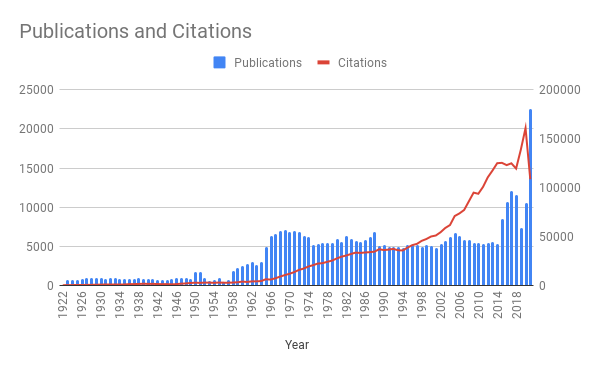
\includegraphics[width=\textwidth]{cites}
    \caption{شبکه عصبی \lr{Feedforward}}
    \label{fig:cites}
\end{figure}

\section{ساختار پژوهش}

در این فصل مقدمه‌ای از متن کاوی بیان شد. در فصل دوم به معرفی مفاهیم پایه پرداخته می‌شود. فصل بعد
مربوط به بررسی کارهای مرتبط می‌باشد و در انتها و در فصل آخر نتیجه گیری و پیشنهاداتی برای بهبود خواهیم داشت.

\chapter{مفاهیم پایه}
\pagebreak
\section{مقدمه}

داده‌کاوی کاربرد بخشی از الگوریتم‌ها برای استخراج الگو‌ها از داده است. متن کاوی در واقع استخراج اطلاعات پر اهمیت از
متن می‌باشد. متن کاوی مجموعه‌ی گسترده‌ای از الگوریتم‌ها و موضوعات مختلفی را در بر می‌گیرد\cite{c9d4fbeac7324056bed5d1cb262a7268}.

\section{پیش پردازش}

در متن کاوی یا به طور کل پردازش‌های مربوط به متون، پیش پردازش یکی از مولف‌های اصلی اکثر الگوریتم‌ها می‌باشد.
به عنوان مثال یک طبقه بندی کننده‌ی متن کلاسیک شامل ۴ بخش پیش پردازش، استخراج ویژگی، انتخاب ویژگی و طبقه بندی است\cite{DBLP:journals/corr/AllahyariPASTGK17a}.

\subsection{توکن سازی}

این عمل در واقع تبدیل کردن متن ورودی و تقسیم آن به قسمت‌های کوچکتر
(کلمه)
است. به این قسمت‌های کوچکتر توکن گفته می‌شود. در
توکن سازی\footnote{Tokenization}
همزمان با به دست آوردن توکن‌ها کاراکتر‌های مشخصی مثل ویرگول، نقطه و غیره نیز حذف می‌شوند.
لیست توکن‌های به دست آمده در مراحل بعدی استفاده می‌شود\cite{DBLP:journals/corr/AllahyariPASTGK17a}.

\subsection{فیلتر کردن}

فیلتر کردن\footnote{Filtering}
زمانی انجام می‌شود که بخواهیم برخی از لغات را از متن پاک کنیم. یکی از فیلتر‌های معمول
کلمات نگهدارنده\footnote{Stop-words}
می‌باشد. این کلمات با تعداد زیادی در متن وجود دارند که بار معنایی خاصی نیز به آن اضافه نمی‌کنند.
به طور کل کلماتی که تعداد دفعات زیادی در یک متن دیده می‌شوند کمک نچندانی برای تشخیص اسناد از یکدیگر می‌کنند
همچنین کلماتی که به ندرت مشاهده می‌شوند نیز بار معنایی خاصی ندارند و می‌توان آن‌ها را از متون حذف کرد\cite{DBLP:journals/corr/AllahyariPASTGK17a}.

\subsection{\lr{Lemmatization}}

این عمل تجزیه و تحلیل واژگان را در نظر می‌گیرد، به عنوان مثال انواع مختلف یک کلمه را یک گروه می‌کند تا در مراحل بعدی
مورد بررسی قرار بگیرند. به بیان دیگر روش‌های
\lr{lemmatization}
سعی در تبدیل هر نوع از کلمات به اصل آن دارند. به عنوان مثال تبدیل فعل به مصدر یا تبدیل اسم جمع به مفرد\cite{DBLP:journals/corr/AllahyariPASTGK17a}.

\subsection{ریشه یابی}

هدف از این کار به دست آوردن ریشه کلمات مشتق شده است. الگوریتم‌های
ریشه یابی\footnote{Stemming}
به زبان وابسطه هستند و این کار محققان را سخت می‌کند. اولین الگوریتم
ریشه یابی
توسط
مارتین پورتر\footnote{\lr{Martin F Porter}}
در
\cite{porter1980algorithm}
منتشر شد که گسترده ترین روش در زبان انگلیسی است\cite{DBLP:journals/corr/AllahyariPASTGK17a}.


\section{روش‌های نمایش}

بساری از شبکه‌های عمیق موجود برای حل مسائل پردازش زبان و گفتار از روش‌های نمایش مختلفی من جمله نتایج
تعبیه کردن کلمات\footnote{\lr{Word embeding}}
به عنوان ورودی برای شبکه‌ی خود استفاده می‌کنند.
تعبیه سازی کلمات
یک تکنیک است برای مدل سازی زبان و یادگیری ویژگی‌های آن برای تبدیل کلمات به بردار اعداد حقیقی پیوسته.
این روش معمولا از روش‌های ریاضیاتی برای تبدیل یک بردار با ابعاد بالا و تنک به یک بردار با ابعاد پایین ولی متراکم استفاده می‌کند.
هر بعد از بردار ساخته شده نمایانگر یکی از ویژگی‌های کلمه است.

یادگیری این بردار‌ها می‌تواند با استفاده از شبکه‌های عصبی عمیق یا فاکتورگیری ماتریسی انجام شود. یکی از روش‌های معمول روش‌
Word2Vec
می‌باشد. این روش با استفاده از شبکه‌هی عصبی عمیق ولی با صرفه‌ی محاسباتی از متن به بردار می‌رسد. یکی دیگر از روش‌های معمول
GloVe
است.
\cite{zhang2018deep}

\subsection{کیف کلمات}

یکی از روش‌های ساده‌ی نمایش متون و جمله‌ها که به خصوص در طبقه‌بندی کاربرد زیادی دارد، روش نمایش
کیف کلمات\footnote{\lr{Bag of Words}}
یا به اختصار
\lr{BoW}
است.

\subsection{GloVe}

\lr{GloVe}
خلاصه شده‌ی 
بردارهای عمومی برای نمایش کلمات\footnote{\lr{Global Vectors for word representation}}
است که یک الگوریتم نظارت نشده برای تبدیل و نمایش کلمات به صورت برداری می‌باشد.
در این الگوریتم داده‌های یک دیتاست به صورت اطلاعات آماری 
هم وقوعی کلمه به کلمه\footnote{\lr{word-word co-occurrence}}
یادگیری می‌شوند و نتیجه‌ی این کار نمایشی خطی و جالب از کلمات
به صورت زیرساختی از فضای برداری است\cite{8844895}.

\section{شبکه‌های عصبی}

یادگیری عمیق درواقع استفاده از 
شبکه‌های عصبی مصنوعی\footnote{\lr{Artificial neural networks}}
به منظور یادگیری انجام کارهای مختلف
با استفاده از شبکه‌ای متشکل از تعدادی لایه عصبی است.

شبکه‌های عصبی با الهام گیری از ساختار و نحوه عملکرد مغز ایجاد شده‌اند. شبکه عصبی مغز تشکیل شده
از تعداد زیادی واحد پردازش اطلاعات می‌باشد که به هر کدام یک از این واحدها نورون گفته می‌شود.
این تعداد زیاد نورون‌ها به نحو و ترتیب خاصی در لایه‌های مختلف جای گرفته‌اند که با یکدیگر به صورت
هماهنگ کار می‌کنند. شبکه‌های عصبی مصنوعی نیز این ساختار را الگو گرفته‌اند و می‌توانند با استفاده از آن‌
و تنظیم وزن‌های اتصال بین نورون‌ها فرایند یادگیری مغز را شبیه سازی کنند و به اصطلاح عمل
یادگیری\footnote{\lr{Learning}}
را انجام دهند.

\begin{figure}[!ht]
    \centering
    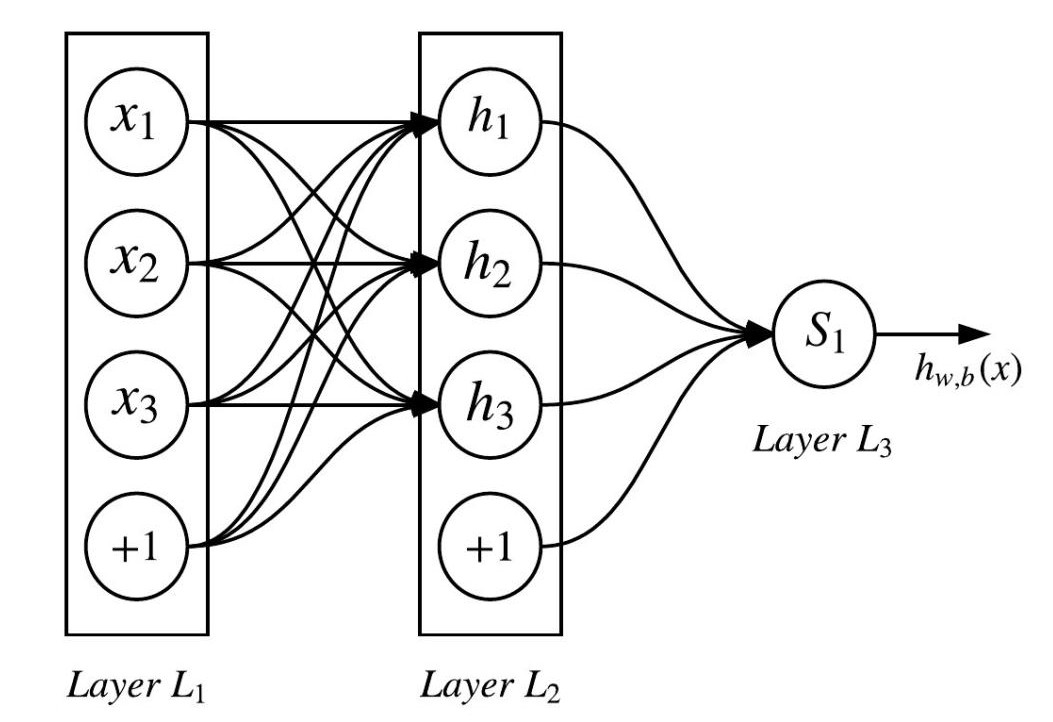
\includegraphics[width=0.80\textwidth]{FFNN}
    \caption{شبکه عصبی \lr{Feedforward}}
    \label{fig:ffnn}
\end{figure}

بر اساس توپولوژی شبکه، شبکه‌های عصبی به دو نوع 
\lr{Feedforward}
و
\lr{Recurrent/Recursive}
تقسیم می‌شوند که می‌توان با ترکیب آن‌ها به شبکه‌های ترکیب شده نیز دست یافت.
یک نمونه ساده از شبکه‌های عصبی
\lr{Feedforward}
در شکل
\ref{fig:ffnn}
آمده‌است. این شبکه دارای ۳ لایه مختلف است، لایه‌ی
\lr{L1}
لایه‌ی ورودی و دریافت کننده وکتور ورودی است. لایه‌ی
\lr{L1}
لایه‌ی میانی و به اصطلاح پنهان که خروجی لایه‌ی اول را گرفته و خروجی آن به لایه‌ی بعدی داده می‌شود. لایه نهایی نیز لایه‌ی
خروجی است که نتیجه‌ی شبکه‌ی عصبی میباشد.
دایره‌ها نشان دهنده‌ی نورون‌ها می‌باشند که به آن‌ها
تابع فعالسازی\footnote{\lr{Activation function}}
نیز گفته می‌شود. خطوط میان هر دو نرون نشان دهنده ارتباطی برای جریان اطلاعات است. هر خط با یک بردار وزن کنترل می‌شود
که میزان اثر گذاری سیگنال بین هر دو نورون را تایین می‌کند.

\subsection{توابع فعال‌سازی}

اگر به درون هر لایه برویم خواهیم دید که این لایه‌ها ورودی لایه‌ی قبلی را گرفته و خروجی را با استفاده از فرمول زیر
محاسبه می‌کند.
\begin{equation}
    f(W^tx)=f(\sum_{i=1}^{inputs} W_ix_i + b)
    \label{formula:activation}
\end{equation}

برای تابع
f
در فرمول
\ref{formula:activation}
کاندیدهای مختلفی وجود دارد که به بررسی برخی از آن‌ها می‌پردازیم.

\subsubsection{سیگموید}

تابع 
سیگموید\footnote{Sigmoid}
یکی از معروف‌ترین توابع برای استفاده جهت
تابع فعال‌سازی
‌است. تابع سیگموید ورودی حقیقی را دزیافت می‌کند و عددی میان ۰ و ۱ تولید می‌کند. این تابع در انواع کاربرد‌های شبکه‌‌های
عصبی استفاده‌ی زیادی دارد و دلیل آن امکان استفاده از مفهوم درست و غلط باینری با استفاده از نتیجه می‌باشد. بدین شکل که
عدد ۱ به معنای درست و عدد ۰ به معنای غلط می‌شود.

\begin{equation}
    sigmoid(W^tx) = \dfrac{1}{1 + exp(W^tx)}
\label{formula:sigmoid}
\end{equation}

اما غیر خطی بودن سیگموید
سبب شده‌است که این تابع به تازگی محبوبیت خود را از دست بدهد زیرا امکان گیر کردن در نقاطی که گرادیان ۰ است وجود دارد.

\begin{figure}[!ht]
    \centering
    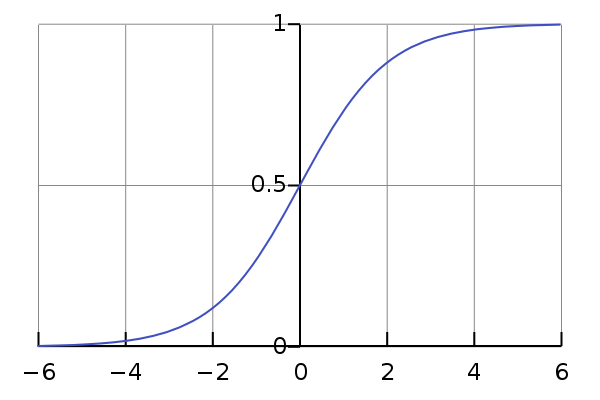
\includegraphics[width=0.80\textwidth]{sigmoid}
    \caption{تابع \lr{sigmoid}}
    \label{fig:sigmoid}
\end{figure}

مشکل دیگر این تابع این است که خروجی آن با مرکزیت ۰ نمی‌باشد. این مسئله سبب به وجود آمدن حالت زیگزاکی
تا در هنگام به روزرسانی وزن‌ها در زمان یادگیری شود.

\subsubsection{تانژانت هیپربولیک}

این تابع در عمل بیشتر ترجیح داده می‌شود زیرا خروجی آن با مرکزیت عدد ۰ است و بازه‌ی خروجی
تانژانت هیپربولیک\footnote{tanh}
بین
\lr{-۱}
تا ۱ می‌باشد.

\begin{equation}
    tanh(W^tx) = \dfrac{e^{W^tx} -e^{-W^tx}}{e^{W^tx} + e^{-W^tx}}
\label{formula:tanh}
\end{equation}

\subsubsection{رلو}

تابع
رلو\footnote{ReLU}
نیز از محبوبیت بالایی برخوردار است و دلیل آن سادگی محاسبه‌ی آن می‌باشد و سرعت آن در رسیدن به نتیجه در زمان
یادگیری میباشد. این تابع در اکثر مواقع نتایجی با عملکرد برابر یا بهتر نسبت به توابع
سیگموید و تانژانت هیپربولیک
دارد و با توجه به سادگی آن معمولا به دو تابع دیگر ترجیح داده می‌شود.

\begin{equation}
    ReLU(W^tx) = \max(0, W^tx)
\label{formula:relu}
\end{equation}

\subsubsection{سافت‌مکس}

از تابع
سافت‌مکس\footnote{Softmax}
می‌توان به عنوان
تایع فعال‌ساز
لایه‌ی اخر استفاده کرد. این تابع حالت کلی تابع تابع
logistic
است که یک بردار
k
بعدی با مقادیر حقیقی را دریافت می‌کند و یک بردار
k
بعدی که هر کدام از عناصر آن عددی بین ۰ و ۱ دارند تولید می‌کند. به طور معمول از
softmax
در لایه‌ی آخر شبکه‌های
Feedforward
و همچنین عمل
کلاس بندی\footnote{Classification}
استفاده می‌شود.

\begin{equation}
   \sigma(X)_j = \dfrac{e^{x_j}}{\sum_{k = 1}^{K} e^{x_k} }  \mbox{ for i = 1,...,n }
\label{formula:softmax}
\end{equation}

\subsection{یادگیری}

برای انجام فرایند یادگیری در یک شبکه‌ی عصبی به طور معمول از
\lr{Stochastic gradient descent}
به همراه
\lr{Backpropagation}
برای کاهش خطای شبکه استفاده می‌شود. گرادیان
خطای شبکه\footnote{\lr{Loss function}}
در ابتدا برای وزن‌های میان آخرین لایه پنهان و لایه خروجی محاسبه می‌شود، به همین ترتیب گرادیان
مربوط به وزن‌های لایه‌های قبلی به صورت بازگشتی با اعمال کردن قاعده زنجیری محاسبه می‌شوند.
با استفاده از این اعداد محاسبه شده وزت‌های هر لایه به روزرسانی می‌شوند. این کار می‌تواند به صورت
پیمایشی\footnote{iterative}
ادامه یابد تا عمل یادگیری به شرایط پایان برسد.

\section{یادگیری عمیق}
در اواخر دهه 90 میلادی جامعه‌ی تحقیقاتی علاقه‌ی خود را به شبکه‌های عصبی از دست داد. دلیل آن هم استفاده از شبکه‌های
با عمق کم\footnote{Shallow}
بود زیرا استفاده از شبکه‌های عمیق\footnote{Deep}
بسیار پیچیده بود و هزینه‌ی محاسباتی زیادی می‌برد.

اما به طور ناگهانی با بهتر شدن سخت افزار و به روز شدن آن‌ها یادگیری عمیق سبب رسیدن به نتایج پیشرفته‌ای در زمینه‌های مختلف شد.
شروع این تغییرات در زمینه بینای ماشین شکل گرفت و سپس به شناسایی گفتار راه یافت. در سال‌های اخیر این روش در تکنیک‌های
مربوط به پردازش زبان و گفتار به شدت مورد استفاده قرار گرفت.

این انقلاب شبکه‌های عمیق می‌تواند دلایل مختلفی داشته باشد اما مهم‌ترین آن‌ها عبارتند از:

\begin{enumerate}
	\item رشد سخت افزار و افزایش قدرت محاسباتی
	\item وجود حجم زیادی از داده به منظور یادگیری
	\item قدرت و انعطاف یادگیری عمیق
\end{enumerate}

به طور خلاصه یادگیری عمیق از به هم چسباندن تعدادی لایه‌ی محاسباتی غیر خطی استفاده می‌کند تا ویژگی‌ها را استخراج و تبدیل کند.
لایه‌های نزدیک به ورودی اطلاعات ساده را استخراج می‌کنند و هر چه به لایه‌های جلو تر نزدیک می‌شویم ویژگی‌های پیچیده تر
از ویژگی‌های ساده استخراج می‌شوند.

\section{رویکردها}

پردازش زبان و گفتار طبیعی\footnote{\lr{Natural Language Processing}}
زیرشاخه‌ای از علوم کامپیوتر، هوش مصنوعی و زبان‌شناسی است که هدف آن درک زبان طبیعی با
استفاده از کامپیوتر است. بسیاری از الگوریتم‌های متن کاوی به طور گسترده از تکنیک‌های
NLP
استفاده می‌کنند\cite{DBLP:journals/corr/AllahyariPASTGK17a}.

\subsection{استخراج اطلاعات}

عمل 
استخراج اطلاعات\footnote{\lr{Information extraction}}
به استخراج اتوماتیک اطلاعات یا حقایق از اسناد بدون ساختار یا نیمه ساختارمند گفته می‌شود.
این عمل معمولا به عنوان نقطه شروعی برای دیگر الگوریتم‌های متن کاوی استفاده می‌شود. به عنوان مثال استخراج
موجودیت‌ها و روابط آن‌ها از متن که می‌تواند اطلاعات معنایی مفیدی به ما بدهند یکی از کار‌های صورت گرفته
در این رویکرد است\cite{DBLP:journals/corr/AllahyariPASTGK17a}.

\subsection{خلاصه سازی متن}

خلاصه سازی متن\footnote{\lr{Text Summarization}}
روشی است که در بسیاری از کاربرد‌های متن کاوی به آن نیاز است تا بتوانند با استفاده از خلاصه‌ی یک متن بلند
یا تعدادی متن به مروری اجمالی دست یافت.

به طور کل دو روش خلاصه سازی وجود دارد،
\lr{extractive summarization}
که خلاصه‌ی به دست آمده شامل واحد‌های اطلاعاتی است که از متون اصلی استخراج شده. در مقابل
\lr{abstractive summarization}
وجود دارد که خلاصه به دست آمده ممکم است شامل اطلاعاتی باشد که در اسناد اصلی موجود نباشند\cite{DBLP:journals/corr/AllahyariPASTGK17a}.

\subsection{تحلیل احساسات و عواطف}

تحلیل عواطف\footnote{\lr{Sentiment analysis}}
یا
استخراج نظرات\footnote{\lr{Opinion Mining}}
در واقع بررسی کامپیوتری نظرات، احساسات، عواطف، ارزیابی‌ها و رفتار مردم در مقابل موجودیت‌هایی
مثل محصولات، سرویس‌ها، سازمان‌ها، اشخاص، مشکلات، رویدادها و مسائل و ویژگی‌های مربوط به آن‌هاست.
رشد سریع
تحلیل عواطف
به دلیل همزمانی آن با به وجود آمدن شبکه‌های اجتماعی مانند فروم‌های نقد و بررسی، بلاگ‌های بحث و جدل،
شبکه‌های اجتماعی، فیسبوک، توییتر و غیره بود زیرا برای اولین بار در تاریخ محققان به حجم عظیمی
از داده‌های نظرات مردم دست یافتند.
\cite{zhang2018deep}

با ظهور تجارت الکترونیک و فروشگاه‌های آنلاین مقدار زیادی از متون مربوط به این حوزه تولید و روز به روز
به حجم این متون اضافه می‌شود. بررسی نظرات و تحلیل احساسات کاربران در این صنعت و با استفاده از داده‌های به دست
آمده از بررسی کالاهای مختلف توسط افراد یا نظرات آن‌ها می‌تواند منجر به پیشرفت تبلیغات و بازاریابی آنلاین شود\cite{DBLP:journals/corr/AllahyariPASTGK17a}.

متونی که برای استخراج عواطف استاده می‌شوند اغلب در سه سطح مورد بررسی قرار می‌گیرند: سطح سند، سطح جمله و سطح جنبه و نمود.
در سطح سند کل یک متن به عنوان منبع بررسی عواطف و احساسات در نظر گرفته می‌شود و مثبت یا منفی بودن آن
به طور کلی بیان می‌شود. برای رسیدن به این هدف فرض می‌شود که کل سند یک واحد اطلاعاتی ساده است و در آن
نظراتی در مورد
\textbf{یک}
مسئله وجود دارد.
\cite{zhang2018deep}

در سطح جمله هر جمله به صورت جدا بررسی می‌شود و تشخیص داده می‌شود که آیا جمله‌ی بررسی شده حاوی نظری مثبت، منفی
یا خنثی است. آنالیز در این سطح رابطه‌ی تنگاتنگی با
طبقه بندی ذهنی\footnote{\lr{Subjectively Classificaion}}
دارد که جمله‌های دارای اطلاعات حقیقی را از جملاتی که حاوی نظرات هستند متمایز می‌کند. اما نکته‌ای که وجود دارد آن است که
نمی‌توان گفت جملاتی که برای انتقال حقایق ساخته شده‌اند حاوی احساسات نیستند.
\cite{zhang2018deep}

تجزیه و تحلیل احساسات مبتنی بر جنبه، در اسناد به دنبال نظرات در مورد بخشی خاص می‌گردد. به عنوان مثال در یک نظر
مربوط به یک کالا، ممکن است فرد از قسمت‌هایی ناراضی و از قسمت‌هایی از کالا راضی باشد، اما به طور کلی نظر مثبتی
ثبت کرده باشد. هدف از این کار بررسی جوانب مختلف یک به اصطلاح
هدف\footnote{target}
است.
\cite{zhang2018deep}

\subsection{خوشه بندی متن}

خوشه بندی\footnote{\lr{Clustering}}
یکی از روش‌های پر استفاده در یادگیری نظارت نشده در متن کاوی است. خوشه بندی عمل تقسیم داده‌ها به گروه‌های
(خوشه)
مختلف است به طوری که داده‌های هر گروه شباهت بیشتری با یکدیگر نسبت به داده‌های گروه‌های دیگر داشته باشند\cite{DBLP:journals/corr/AllahyariPASTGK17a}.


\subsection{طبقه‌بندی متن}

طبقه بندی متن\footnote{\lr{Text Classification}}
یک موضوع کلاسیک در پردازش زبان‌های طبیعی است که در آن نیاز است تا اسناد مختلف را در گروه‌های
از پیش تعیین شده‌ی موجود قرار داد\cite{c9d4fbeac7324056bed5d1cb262a7268}.
این موضوع به دلیل کاربرد‌های مختلف آن مانند جست و جو در وب، بازیابی اطلاعات،
رتبه بندی و طبقه بندی اسناد از اهمیت بالای برخوردار است\cite{joulin2016fasttext}.

در سال‌های اخیر نشان داده شده است که شبکه‌های عصبی که می توانند از ترتیب کلمات استفاده کنند،
برای دسته بندی متن موثر هستند\cite{iyyer-etal-2015-deep}.

\subsection{ترجمه ماشینی عصبی}
ترجمه ماشینی عصبی\footnote{\lr{Neural Machine Translation}}
یک روش برای رفع نواقض ترجمه ماشینی سنتی است. در این روش متن ورودی به صورت مستقیم و
\lr{end-to-end}
برای ترجمه یادگیری و به متن خروجی تبدیل می‌شود.
به طور کلی شبکه‌هایی که این مسئولیت را بر عهده دارند از دو شبکه
RNN
تشکیل شده‌اند. یکی برای پردازش متن و دیگری برای تولید متن خروجی.
بسیاری از اوقات از مکانیزم توجه برای این کار استفاده می‌شود.
این کار سبب بهبود عملکرد در برابر جملات و دنباله‌های طولامی می‌شود.

مشکلات اصلی استفاده از شبکه‌های عمیق به جای استفاده از مدل‌های آماری به سه دسته‌ی کلی طبقه بندی می‌شود.
اولین مشکل زمان زیاد مربوط به بخش یادگیری است که این مسئله برای تمام روش‌های شبکه‌های عمیق وجود دارد.
مشکل بعدی عدم ثبات در مواجهه با کلماتی است که به ندرت استفاده می‌شوند.
و آخرین مشکل آن است که این نوع شبکه‌ها در برخی موارد قادر به ترجمه‌ی تمام کلمات ورودی نیستند.\cite{wu2016google}

هدف اصلی از انجام این کار در واقع همان هدف کلی پردازش زبان و گفتار طبیعی است، شناخت کامل جملات
و گفتار انسان‌ها. این مسئله در سال‌های اخیر توجه زیادی را به خود جلب کرده‌است. دلیل ان هم سادگی
مدل‌ها نسبت به مدل‌های آماری مثل ترجمه ماشینی بر اساس عبارت\footnote{\lr{Phrase-Based Statistical Machine Translatio}}
و همجنین قابلیت استخراج وابستگی‌ها درون جملات توسط مدل‌های ارائه شده، است.
\cite{yang2020survey}

\section{شبکه‌ها}

\subsection{اتوانکودرها}

شبکه عصبی
اتوانکودر\footnote{Autoencoder}
یک شبکه سه لایه است که اندازه ابعاد خروجی آن با ابعاد ورودی برابر است. شکل 
\ref{fig:autoencoder}
ساختار یک اتوانکودر را نشان می‌دهد.

\begin{figure}[!ht]
    \centering
    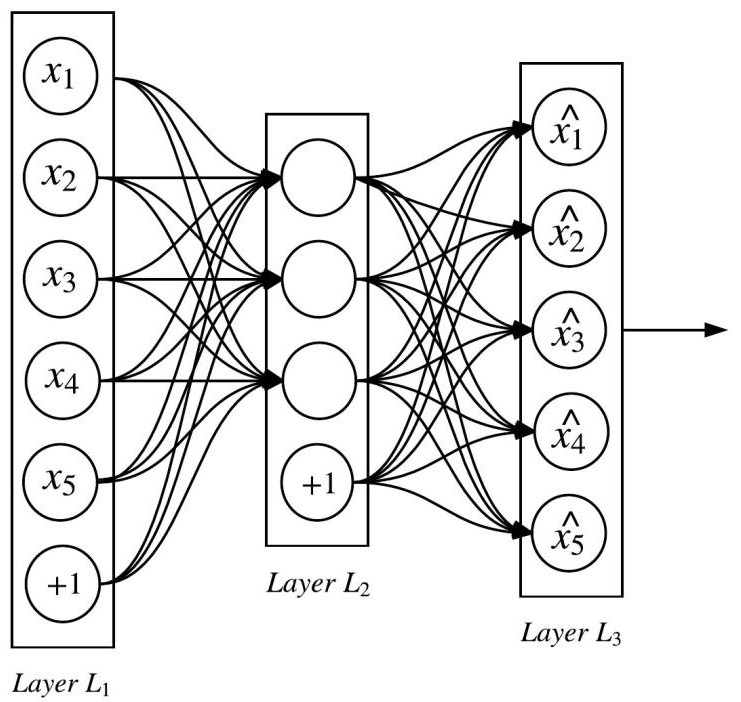
\includegraphics[width=0.80\textwidth]{autoencoder}
    \caption{شبکه عصبی اتوانکودر}
    \label{fig:autoencoder}
\end{figure}

در این نوع شبکه ورودی ابتدا به یک لایه‌ی پنهان به اصطلاح
رمزگذاری\footnote{encode}
می‌شوند سپس خروجی این لایه 
رمزگشایی\footnote{decode}
می‌شود و به لایه‌ی خروجی می‌رسد. هدف این نوع شبکه‌ها یادگیری ارائه‌ و نمایش ورودی می‌باشد. اتوانکودرها قادر به یادگیری
نمایش‌های غیر خطی می‌باشدن که نسبت به روش‌های خطی مثل
PCA
یا
LSA
از برتری برخوردار است.

\subsection{طبقه بندی کننده خطی}

طبقه بندی کننده‌ی خطی\footnote{\lr{Linear Classifier}}
به عنوان روشی قوی و پایه‌ای برای مسائل طبقه بندی متون مورد قبول همه واقع شده‌اند. بر خلاف
سادگی ساختاری این شبکه‌ها، در صورت استفاده از ویژگی‌های درست و مناسب می‌توانند به نتایج مطلوبی
دست‌ یابند. ویژگی دیگر مهم این شبکه‌ها عملکرد مناسب در هنگام استفاده از دیتاست‌های بزرگ می‌باشد\cite{joulin2016fasttext}.

طبقه بندی کنندگان خطی پارامترها را بین کلاس‌ها و ویژگی‌ها به اشتراک نمی‌گذارند و این سبب ضعیف عمل
کردن در امر
کلی سازی\footnote{\lr{Generalization}}
هنگامی که تعداد کلاس‌ها بالا می‌رود و برخی از کلاس‌ها نمونه‌های کمی دارند می‌شود.

\subsection{شبکه کانولوشنال}

\lr{CNN}\footnote{\lr{Convolutional Neural Network}}
یک شبکه
\lr{feedforward}
با لایه‌های کانولوشنال در هم تنیده شده با لایه‌های
\lr{pooling}
است. در این شبکه‌ها لایه‌ی کانولوشنال هر بخش از دیتای ورودی شبکه یا خروجی لایه‌ی قبل را به یک بردار 
تبدیل می‌کند که این انر امکان پردازش موازی را نیز فراهم می‌کند\cite{iyyer-etal-2015-deep}. شکل
\ref{fig:cnn}
یک شبکه کانولوشنال ساده را نشان می‌دهد.

بسیاری از محققان بدین مسئله دست یافته‌اند که استفاده از 
شبکه‌های کانولوشنال\footnote{\lr{ConvNets}}
برای استخراج اطلاعات از سیگنال‌های پردازش نشده بسیار مناسب می‌باشد. به همین دلیل این شبکه‌ها
استفاده‌ی زیادی در
بینایی ماشین\footnote{\lr{Computer Vision}}
،
تشخیص گفتار\footnote{\lr{Speech Recognition}}
و غیره دارند\cite{c9d4fbeac7324056bed5d1cb262a7268}.

بسیاری برای کار کردن در زمینه متن‌کاوی، به متون به شکل سیگنال‌های پردازش نشده نگاه می‌کنند
تا بتوانند با استفاده از
\lr{ConvNets}
اطلاعات ارزشمند و مختلفی از متون استخراج کنند\cite{c9d4fbeac7324056bed5d1cb262a7268}.

CNN 
یک نوع شبکه‌ی عصبی است که می‌تواند از ساختار درونی و ازتباطات داده‌ها استفاده کند.
به عنوان مثال ساختار ۲-بعدی تصاویر به این شبکه‌ها در رسیدن به پاغسخ بهتر کمک شایانی می‌کنند.
در متون نیز این شبکه‌ها ارتباطات کلمات و حروف درون جمله را بررسی می‌کنند.
\cite{johnson-zhang-2015-effective}

\begin{figure}[!ht]
    \centering
    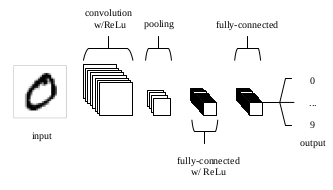
\includegraphics[width=0.80\textwidth]{CNN}
    \caption{ساختار یک شبکه عصبی کانولوشنال ساده}
    \label{fig:cnn}
\end{figure}

\subsection{\lr{RNN}}

\lr{RNN}
مخفف
\lr{Recurrent Neural Network}
می‌باشد. این شبکه‌ها دارای حلقه‌های
بازخورد\footnote{\lr{feedback}}
در لایه‌های خود هستند. همین ویژگی اجازه می‌دهد تا داده را با گذشت زمان در حافظه‌ی خود نگه دارند.
اما یادگیری این نوع شبکه‌ها برای مسائلی که نیاز به یادگیری وابستگی‌های طولانی مدت دارند سخت است.

در یک شبکه
\lr{RNN}
به طور معمول در انجام فعالیت‌های مربوط به پردازش متن هر واحد شبکه کلمه‌ی ورودی را به همراه
خروجی تولید شده‌ی خود برای کلمه‌ی گذشته را پردازش می‌کند. این ویژگی از پردازش موازی جلوگیری می‌مند\cite{iyyer-etal-2015-deep}.

در تحقیقی که برای مقایسه
\lr{RNN}
و
\lr{CNN}
جهت رسیدن به دستورعملی ابتدایی برای انتخاب شبکه عمیق در راستای انحام فعالیت‌های مربوط به زبان طبیعی
انجام شد، نشان داده شد که شبکه‌های
\lr{RNN}
در تعداد زیادی از مسائل عملکردی مناسب و قوی دارند. همچنین در این تحقیق بر اهمیت زیاد به دست آوردن
مقادیر مناسب
اندازه دسته ورودی به شبکه\footnote{\lr{batch size}}
و
اندازه لایه‌های مخفی\footnote{\lr{hidden size}}
تاکید بسیار شده‌است\cite{8844895}.

\begin{figure}[!ht]
    \centering
    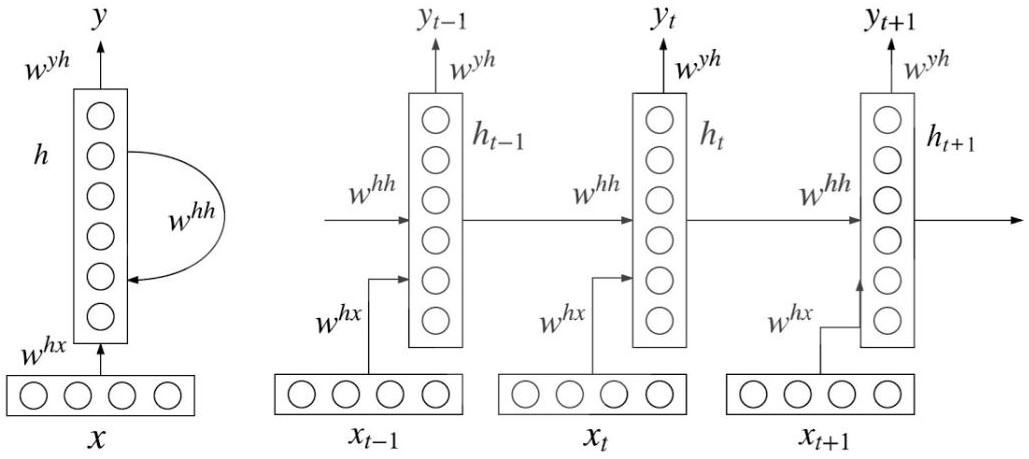
\includegraphics[width=0.7\textwidth]{rnn}
    \caption{ساختار یک شبکه عصبی Recurrent}
    \label{fig:rnn}
\end{figure}

\subsection{LSTM}

\lr{LSTM}
مخفف
حافظه بلند کوتاه مدت\footnote{\lr{Long-Short Term Memory}}
است. این شبکه‌ها در واقع نوع خاصی از شبکه‌های
\lr{RNN}
هستند که علاوه بر ساختار اصلی از 
واحد‌های ویژه‌ای\footnote{\lr{special units}}
استفاده می‌کنند. این واحدها در خود یک 
سلول حافظه\footnote{\lr{memory cell}}
جای داده‌اند که می‌تواند داده را برای مدت زمان طولانی در خود ذخیره کند.

مجموعه‌ای از گیت‌ها جهت تنظیم داده‌های ورودی به حافظه، داده‌های خروجی و داده‌های فراموش شده طراحی
شده‌اند. این روش طراحی به مدل اجاره می‌دهد که وابستگی‌های طولانی مدت‌تری را یادگیری کند\cite{8844895}.

\begin{figure}[!ht]
    \centering
    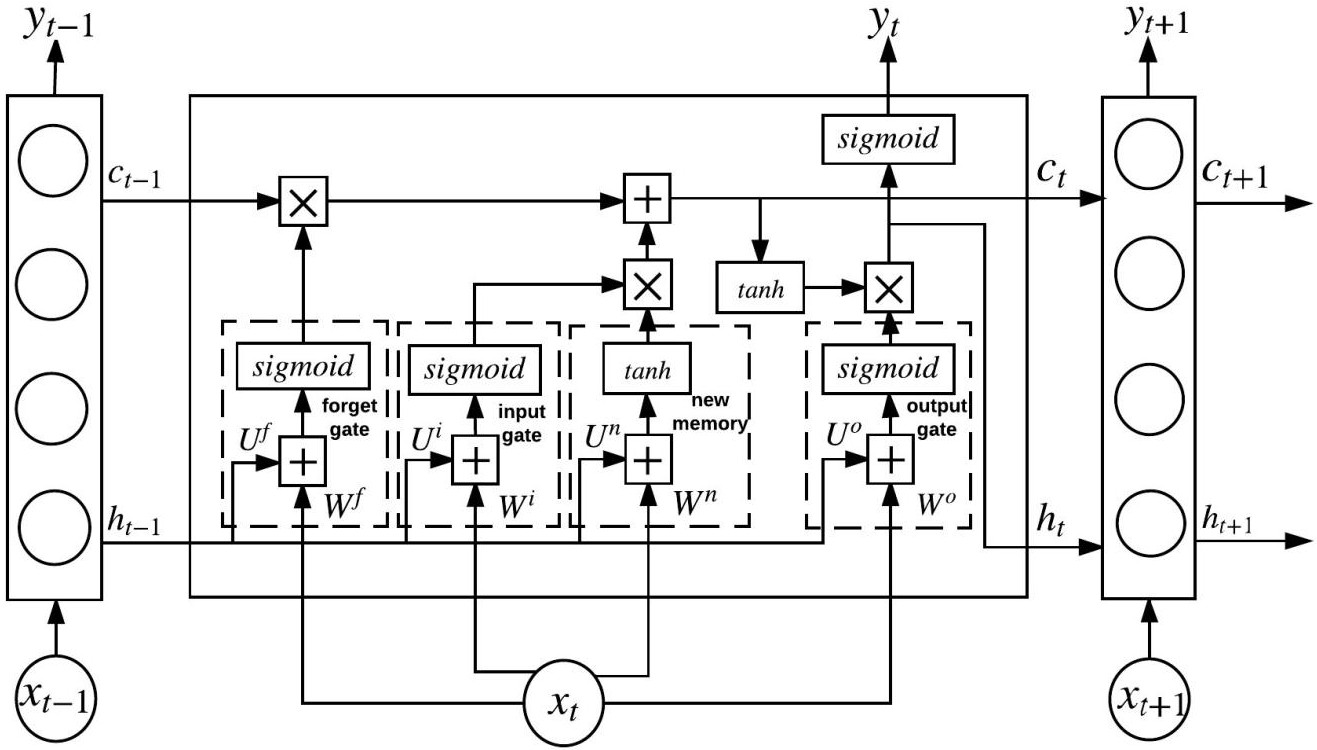
\includegraphics[width=0.7\textwidth]{lstm}
    \caption{ساختار یک شبکه عصبی LSTM}
    \label{fig:lstm}
\end{figure}

در پردازش زبان و گفتار طبیعی از دو شبکه
LSTM
و
CNN
بسیار استفاده می‌شود. اما این دو شبکه هرکدام داده‌های ورودی را به سبک خود مورد بررسی قرار می‌دهند. شکل
\ref{fig:LSTMvsCNN}
این تفاوت را نشان می‌دهد.

\begin{figure}[!ht]
    \centering
    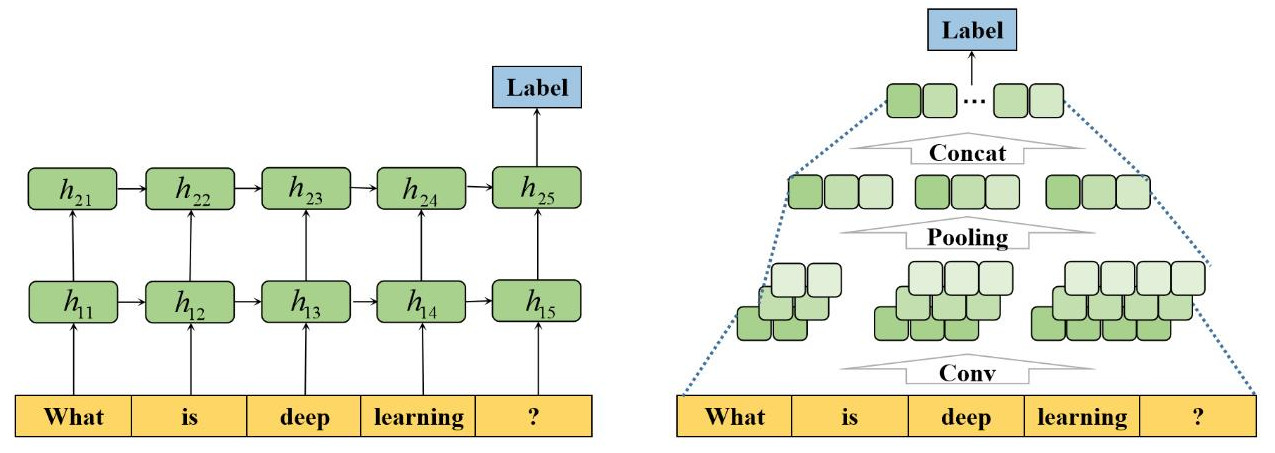
\includegraphics[width=0.8\textwidth]{LSTMvsCNN}
    \caption{تفاوت دو شبکه کانولوشنان و LSTM در پردازش داده}
    \label{fig:LSTMvsCNN}
\end{figure}

\subsection{مکانیزم توجه}

اگرچه شبکه‌های
RNN
و
LSTM
می توانند واستگی‌های زمانی را درک کنند اما در عمل کار کردن با این نوع وابستگی‌ها بسیار مشکل می‌باید. برای گذر از این
مشکل تکنیکی به نام
مکانیزم توجه\footnote{\lr{attention mechanism}}
معرفی شد. این تکنیک با الهام گیری از مکانیزم توجه در سیستم بینایی انسان‌ها ساخته شده‌است. توجه بینایی انسان قادر است
تا بر بخشی از تصویر تمرکز کند و آن را با وضوح و رزلوشن بالا ببیند در حالی که اطراف این ناحیه با رزلوشن پایین تری دیده می‌شود.
این ناحیه تمرکز با گذر زمان تنظیم می‌شود.

در پردازش زبان و گفتار مکانیزم توجه به مدل این اجازه را می‌دهد تا توجه خود را به آن چه تا کنون توسط متن ورودی تولید شده‌است
متمرکز کند. بر خلاف
RNN
و
LSTM
که متن را به یک بردار با طول ثابت تبدیل می‌کنند.

\subsection{شبکه‌های \lr{Transformer}}
به تازگی شبکه‌های
Transformer
نتایج و موفقیت‌های زیادی در بسیاری از کاربرد‌های هوش مصنوعی مثل پردازش زبان و گفتار، بینایی ماشین و
پردازش صدا و امواج کسب کرده‌اند. همین مسئله سبب آن شده‌است که محققین زیادی کار بر روی این شبکه‌ها را آغاز کنند
در نتیجه پیشرفت‌های چشم‌گیری حاصل شده‌است.

Transformer
ها یکی از روش‌های یادگیری عمیق
هستند که استفاده‌های مختلفی از آن‌ها می‌شود. این شبکه‌ها در اصل به عنوان مدلی برای داده‌های دنباله‌ای به خصوص
ترجمه ماشینی ارائه شدند. پژوهش‌های بعدی نشان داد که مدل‌های از پیش
train
شده‌ی مبتنی بر
transformer
ها قادر به کسب نتایج فوق‌العاده در بسیاری از مسائل هستند. همین مسئله باعث شد تا شبکه‌های
transformer
به عنوان معماری پایه‌ی بسیاری از مسائل پردازش زبان و گفتار طبیعی استفاده شوند.

مدل ابتدایی که یک مدل
sequence-to-sequence
است شامل یک
encoder
و یک
decoder
می‌باشد که هر کدام از این بخش‌ها تشکیل شده از تعدادی بلاک دقیقا شبیه به هم هستند. هر
encoder
به طور کلی تشکیل شده از یک ماژول
multi-head
و یک ماژول
self-attention
و یک شبکه 
feed-forward
است. در مقابل در بلاک
decoder
یک ماژول
cross-attention
بین هر دو جفت ماژول از ماژول‌های گفته شده قرار دارد.\cite{lin2021survey}

\begin{figure}[!ht]
    \centering
    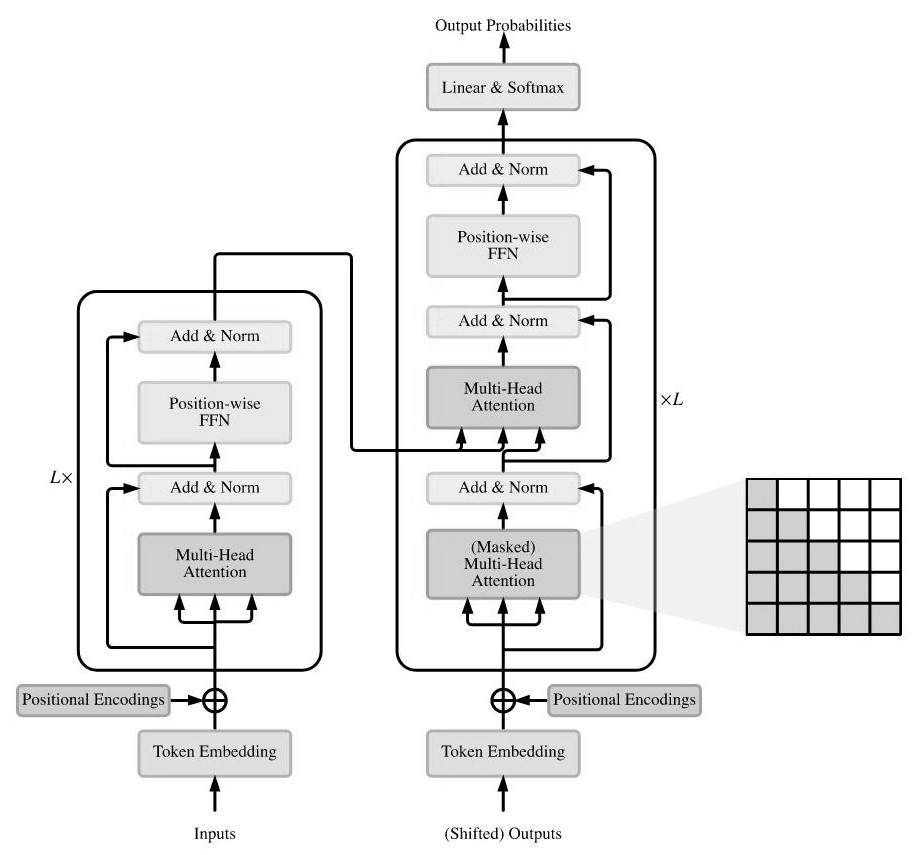
\includegraphics[width=0.8\textwidth]{transformer}
    \caption{ ساختار شبکه transformer }
    \label{fig:transformer}
\end{figure}

\subsubsection{شبکه‌ی BERT}

شبکه‌ی
BERT
که مخفف
\lr{Bidirectional Encoder Representations from Transformers}
است در بسیاری از موارد و مسائل مربوط به پردازش زبان و گفتار طبیعی استفاده می‌شود.
این شبکه طوری طراحی شده‌است تا با داده‌های برچسب گذاری نشده کار کند. همین مسئله بائث می‌شود تا بتوان با استفاده از
fine-tuning
مدل
BERT
را در بسیاری از موارد به خصوص جواب دادن به سوالات مورد استفاده قرار داد. 

این مدل از دو مرحله‌ی
pre-training
و
fine-tuning
تشکیل شده‌است. در مرحله‌ی اول مدل با استفاده از داده‌های برچسب گذاری نشده یادگیری می‌شود و در مرحله بعدی پارامتر‌های
یادگیری شده به مدل داده می‌شود و با استفاده از داده‌های برچسب گذاری شده و یک لایه‌ی نهایی
fine-tune
می‌شود. اگرچه پارامتر‌های یادگیری شده ثابت هستند اما این شبکه برای دست‌یابی به مدل مناسب باید برای هر مسئله
fine-tune
شود. مزیت
BERT
نیز همین است که ساختار شبکه‌های مختلف با توجه به لایه‌ی آخری که اضافه می‌شود شباهت‌های بسیاری دارند و تنها نیاز است
تا تغییرات کوچکی ایجاد شود.

ساختار شبکه‌ی
transformer
به کار رفته به مدل اصلی بسیار شبیه است. اما معماری کلی شبکه به صورت یک شبکه‌ی چندلایه‌ی
\lr{transformer encoder}
است. 

برای آن که این شبکه قادر به انجام وظایف زیادی باشد ورودی شبکه طوری طراحی شده‌است تا امکان دریافت جمله و جفت جمله
را داشته باشد. البته در اینجا جمله به معنای متن ورودی است.
در این شبکه برای توکن کردن داده از روش
WordPiece
با تعداد ۳۰۰۰۰ لغت استفاده شده‌است. اولین توکن هر دنباله نیز
CLS
در نظر گرفته شده تا با استفاده از آخرین
\lr{hidden state}
مربوط به این توکن بتوان وظایف مربوط به طبقه بندی را انجام داد.
همچنین در صورتی که داده به صورت جفت جمله باشد، هر دوی این جملات با هم ترکیب شده و به صورت یک دنباله در می‌ایند.
برای آن که این دو جمله در دنباله تولید شده از هم متمایز باشند از توکن
SEP
میان آن‌ها استفاده می‌شود. در انتها در توکن ورودی به ترکیبی از توکن،
segment
مربوط به آن(جمله‌ی اول یا دوم)
و همچنین مکان توکن در جمله تبدیل می‌شود.

به منظور
pre-train
کردن شبکه‌ به جای استفاده از روش‌های سنتی چپ به راست یا راست به چپ از دو مسئله بدون نظارت بهره گیری می‌شود.

مسئله‌ی اول
\lr{Masked Language Modeling}
است. برای این کار بخشی از توکن‌های ورودی به اصطلاح
mask
می‌شوند. این کار به صورت رندم و با درصدی از پیش تعیین شده صورت می‌گیرد. سپس شبکه به پیشبینی توکن‌های پنهان شده
که با 
MASK
نشان داده می‌شوند می‌پردازد. بردار نهایی به دست آمده از این کار به یک تابع
سافت‌مکس
داده می‌شود. در این مدل ۱۵ درصد توکن‌ها به صورت رندم پنهان‌سازی می‌شوند و همچنین به جای پیشبینی کل دنباله تنها
توکن‌های پنهان شده پیشبینی می‌شوند. هنگام پنهان کردن توکن‌ها ۳ اتفاق ممکان است رخ دهد. با احتمال ۸۰ درصد توکن
پنهان می‌شود. با احتمال ۱۰ درصد توکن پیگری که به صورت رندم انتخاب شده‌است جایگذاری می‌شود. و با احتمال ۱۰ درصد
بدون تغییر باقی می‌ماند. سپس مرحله پیشبینی با بهره گیری از
\lr{cross entropy loss}
انجام می‌شود.

مسئله‌ی دوم پیشبینی جمله‌ی بعدی است. بسیاری از مسائل پردازش زبان و گفتار مانند پاسخ دهی به سوالات نیازمند داشتن
دانشی از ارتباط بین دو جمله است. برای آن که شبکه درکی از ارتباط میان دو جمله داشته باشد شکه با داده‌های دو جمله‌ای
یادگیری می‌شود. برای این کار دو جمله با توجه به ساختار گفته شده به شبکه داده می‌شود. در نصف مواقع جمله‌ی دوم
واقعا جمله‌ای است که در پی جمله‌ی اول می‌آید ولی در باقی موارد جمله‌ی دوم به صورت تصادفی از میان داده‌های موجود
انتخاب می‌شود.

برای انجام این دو وظیفه از دیتاست‌های
BooksCorpus
و
Wikipedia
استفاده شده‌است. 

\begin{figure}[!ht]
    \centering
    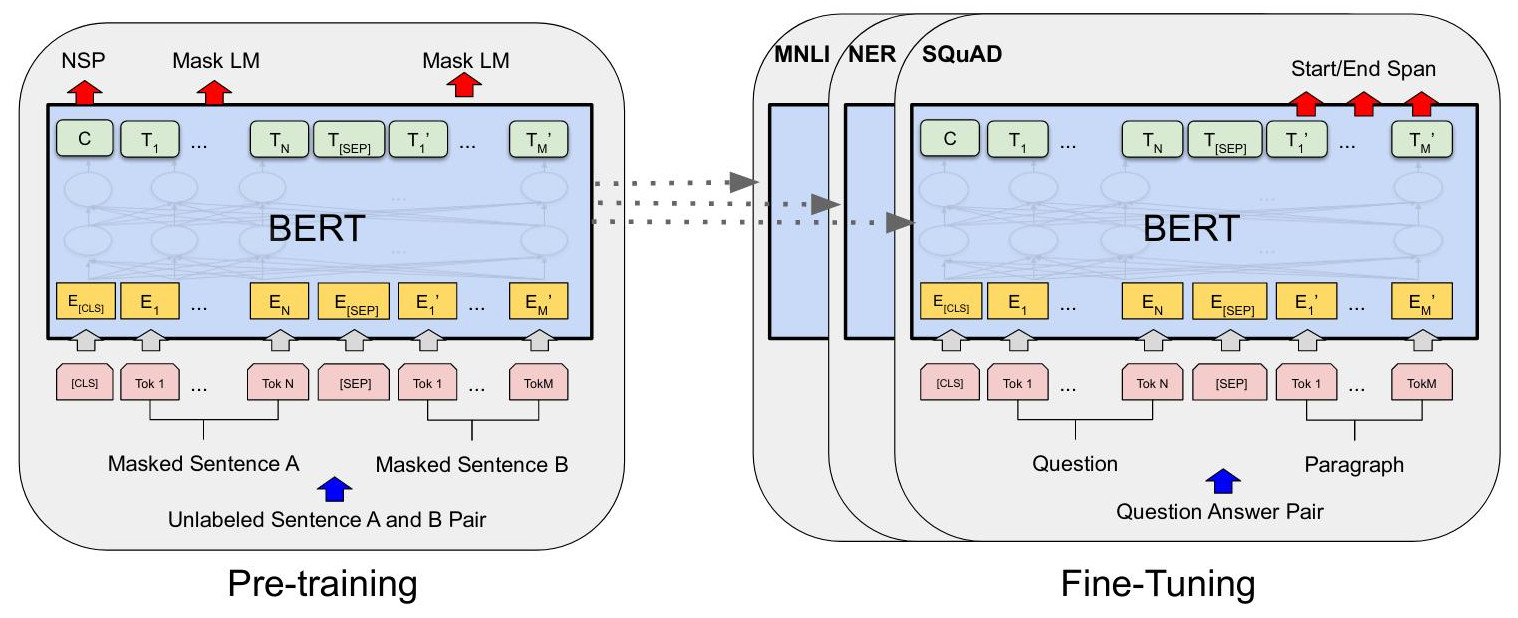
\includegraphics[width=0.8\textwidth]{bert}
    \caption{ ساختار شبکه bert }
    \label{fig:bert}
\end{figure}

بخش بعدی
fine-tune
کردن شبکه است که این کار به خاطر وجود مکانیزم توجه در شبکه به راحتی انجام می‌شود.
در واقع ورودی و خروجی‌های مورد نظر به شبکه داده می‌شود و شبکه به صورت
end-to-end
عملیات
fine-tuning
را انجام می‌دهد.

در مقایسه با
pre-training
علمیات
fine-tuning
هزینه‌ی کمتری می‌برد. به طوری که برای رسیدن به جواب با استفاده از یک
GPU
تنها چند ساعت نیاز است.\cite{devlin2018bert}
شبکه‌ی
BERT
از دو مدل
OpenAI GPT
و
ELMo
الهام گرفته شده و ویژگی‌های مثبت هر کدام را استفاده کرده تا به ساختاری جدید دست یابد. شکل
\ref{fig:BERTvsOTHER}
مقایسه‌ای از ساختار این سه شبکه است.

\begin{figure}[!ht]
    \centering
    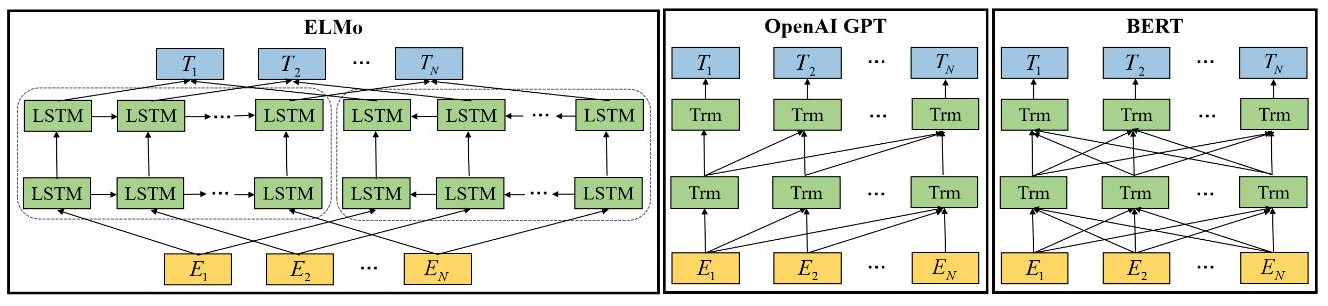
\includegraphics[width=1\textwidth]{BERTvsOTHER}
    \caption{ مقایسه سه شبکه Transformer }
    \label{fig:BERTvsOTHER}
\end{figure}

\subsection{شبکه‌های حافظه‌ای}
شبکه‌های حافظه‌ای\footnote{\lr{Memmory Networks}}
که به طور خلاصه
MenNN
نیز نوشته می‌شوند در ابتدا برای پاسخ دهی به سوالات ارائه شدند. این شبکه دارای تعدادی کامپوننت استنباطی در کنار یک
حافظه‌ی بلند مدت بزرگ است که به عنوان منبع دانایی عمل می‌کند. وظایف کلی کامپوننت‌ها به این شکل است. کامپوننت
I
ورودی را به نمایش ویژگی‌ها تبدیل می‌کند. کامپوننت بعدی یعنی
G
بر اساس ورودی‌های دریافتی جدید حافظه را به روزرسانی می‌کند. کامپوننت
O
در واقع وظیفه‌ی تولید خروجی را بر عهده دارد و کامپوننت
R
خروجی تولید شده را به فرمت مورد نظر تبدیل می‌کند. جدول
\ref{tab:MemNN-vs-others}
مقایسه‌ی این مدل به دو شبکه
RNN
و
LSTM
را در دو مسئله با سختی‌های متفاوت نشان می‌دهد.
\cite{zhang2018deep}

\begin{table}[!ht]
    \begin{small}
    \begin{center}
      \begin{latin}
      \begin{tabular}{|l||l|l|l||l|l|}
        \hline
         & \multicolumn{3}{c|}{Difficulty 1} & \multicolumn{2}{c|}{Difficulty 5} \\
        \hline
        Method & actor w/o before & actor & actor+obj & actor & actor+obj \\
        \hline
        RNN & 100\% & 60.9\% & 27.9\% & 23.8\% & 17.8\% \\
        LSTM & 100\% & 64.8\% & 49.1\% & 35.2\% & 29.0\% \\
        \hline
        MemNN k= 1 & 97.8\% & 31.0\% & 24.0\% & 21.9\% & 18.5\% \\
        MemNN k= 1 & 99.9\% & 60.2\% & 42.5\% & 60.8\% & 44.4\% \\
        MemNN k= 2 & 100\% & 100\% & 100\% & 100\% & 99.9\% \\
        \hline
      \end{tabular}
      \end{latin}
      \caption{مقایسه عملکرد سه مدل حافظه‌ای}
      \label{tab:MemNN-vs-others}
    \end{center}
    \end{small}
\end{table}


\chapter{تاریخچه پژوهش}
\pagebreak

\begin{landscape}
\begin{figure}[!ht]
\begin{latin}
\begin{tiny}
\begin{noindent}
\begin{forest}
    for tree = { draw, align=center },
    before typesetting nodes={
        where content={}{coordinate}{},
    },
    forked edges,
    [Text Mining
        [Classification
            [Sentiment Analysis
                [CNN \\
                    \cite{dos2014deep} \\
                    \cite{wang-etal-2016-combination} \\
                    \cite{guggilla-etal-2016-cnn}
                ]
                [GRU \\
                    \cite{72Zhang_Zhang_Vo_2016}
                ]
                [LSTM \\
                    \cite{xu2016cached} \\
                    \cite{yin-etal-2017-document} \\
                    \cite{zhou-etal-2016-attention} \\
                    \cite{wang-etal-2016-combination} \\
                    \cite{guggilla-etal-2016-cnn} \\
                    \cite{teng-etal-2016-context} \\
                    \cite{70tang-etal-2016-effective} \\
                    \cite{71ruder-etal-2016-hierarchical} \\
                    \cite{73wang-etal-2016-attention} \\
                    \cite{74YANGATT} \\
                    \cite{79ma2017interactive}
                ]
                [MemNN \\
                    \cite{ijcai2017-311} \\
                    \cite{76tang2016aspect}
                ]
                [RecNN \\
                    \cite{68dong-etal-2014-adaptive}
                ]
            ]
            [CNN \\
                \cite{johnson-zhang-2015-effective} \\
                \cite{conneau2016very} \\
                \cite{johnson-zhang-2017-deep}
            ]
            [GRU \\
                \cite{yang-etal-2016-hierarchical} \\
                \cite{dieng2016topicrnn}
            ]
            [LSTM \\
                \cite{graves2005framewise} \\
                \cite{liu2016recurrent} \\
                \cite{miyato2017adversarial} \\
            ]
            [Transformers \\
                \cite{schmidt2020data}
            ]
        ]
        [Neural Machine Translation
            [CNNN \\
                \cite{kalchbrenner2013recurrent} \\
                \cite{gehring2017convolutional}
            ]
            [LSTM \\
                \cite{wu2016google} \\
                \cite{sutskever2014sequence} \\
                \cite{zhou2016deep} \\
                \cite{wu2016googles}
            ]
            [Transformers \\
                \cite{bapna2018training} \\
                \cite{wang2019learning}
            ]
        ]
        [Information extraction
            [CNN \\
                \cite{ma2016endtoend} \\
                \cite{katti2018chargrid}
            ]
            [Transformers \\
                \cite{dai2019transformerxl} \\
                \cite{yang2020xlnet} \\
                \cite{denk2019bertgrid}
            ]
            [LSTM \\
                \cite{lample2016neural} \\
                \cite{ma2016endtoend}
            ]
        ]
        [Text Summarization
            [GRU \\
                \cite{zhang2018extractive}
            ]
            [LSTM \\
                \cite{song2019abstractive} \\
                \cite{li2017cascaded} \\
                \cite{amplayo2021informative} \\
                \cite{liu2018generating}
            ]
            [CNN \\
                \cite{song2019abstractive} \\
                \cite{ziqiang2015prior}
            ]
            [Transformers \\
                \cite{liu2018generating} \\
                \cite{liu2019hierarchical}
            ]
        ]
        [Clustering \\
            [CNN \\
                \cite{Xu2017} \\
                \cite{fan2018neural}
            ]
            [LSTM \\
                \cite{zhou2019endtoend} \\
                \cite{fan2018neural}
            ]
        ]
    ]
\end{forest}
\end{noindent}
\end{tiny}
\end{latin}
\end{figure}
\end{landscape}

\pagebreak

\section{مقدمه}

دراین بخش به بررسی روش‌های ارائه شده با رویکردها و شبکه‌های مختلف پرداخته می‌شود.
مدل‌های ارائه شده در این بخش با توجه به سال ارائه‌ی مقاله و همچنین تعداد نفراتی که از مقالات استفاده کرده‌اند
یا به صورت مستقیم یا در بخش بررسی چند مقاله مرور می‌شوند. همچنین این دو معیار میزان پرداختن به مقالات را نیز تعیین
می‌کنند.

\section{روش‌های بر پایه رویکرد طبقه بندی متن}

\subsubsection{Seq-CNN و ‌BOW-CNN}

ترتیب کلمات درون متون قطعا تاثیر بسیار زیادی در معنا و مفهوم و در نهایت این که هر متن در چه کلاسی قرار می‌گیرد
تاثیر بسیار زیادی دارد. اما روش‌های بر مبنای
BOW
از این ویژگی استفاده‌ای نمی‌کنند. زیرا بردار حاوی اطلاعات تنها این که چه کلماتی در متن استفاده شده‌اند را نمایش می‌دهند
و ترتیب و جایگاه کلمات نادیده گرفته می‌شوند. در این مقاله برای آن که از این ترتیب بهره‌گیری و استفاده شود از شبکه‌ی عصبی
کانولوشنال
استفاده شده‌است. استفاده از
CNN
سبب می‌شود تا بتوان از ساختار ترتیبی متون بهره برد تا هر بخش از شبکه‌ی کانولوشنی مسئولیت پردازش بخشی از متن
یا دنباله‌ای از کلمات را داشته باشد. شکل
\ref{fig:cnn-in-text}
این عمل را نشان می‌دهد.

\begin{figure}[!ht]
    \centering
    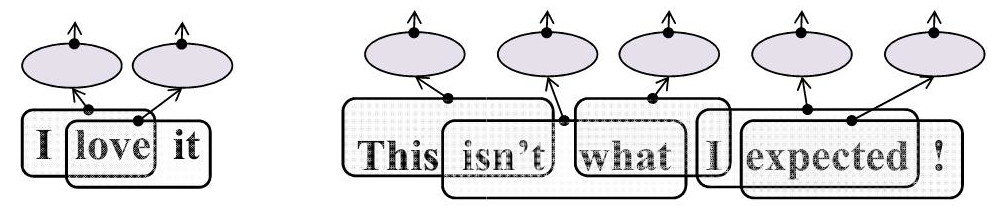
\includegraphics[width=0.8\textwidth]{cnn-in-text}
    \caption{ استفاده از شبکه‌ی کانولوشنی به منظور بهره‌گیری از ترتیب کلمات }
    \label{fig:cnn-in-text}
\end{figure}

به منظور این کار شبکه‌ی کانولوشنال به صورت مستقیم با بردار ورودی سر و کار دارد و در واقع به جای استفاده از
روش‌های
embeding
، خود شبکه این کار ار یاد می‌گیرد. دو نوع شبکه
seq-CNN
و
BOW-CNN
معرفی شد و نشان داده شد که شبکه‌ی اول در تحلیل عواطف بهتر عمل می‌کند و روش دوم در طبقه بندی بر اساس موضوع.
\cite{johnson-zhang-2015-effective}

\subsubsection{HN-ATT}

طبقه بندی و کلاس بندی اسناد جزو عمل‌های اولیه در پردازش زبان و گفتار طبیعی است.
در
\cite{yang-etal-2016-hierarchical}
با ارائه شبکه توجه سلسله مراتبی\footnote{\lr{Hierarchical Attention Network}}
سعی بر دریافت و بررسی دو ویژگی مهم متون و اسناد دارد. یکی آن که اسناد ساختار سلسله مراتبی دارند، 
کلمات جمله‌ها را تشکیل می‌دهند و جملات اسناد را. به همین منظور در این مقاله ساختاری از جملات به دست می‌اید
و سپس از این ساختار به ساختار اسناد می‌رسند.

ویژگی بعدی آن است که کلمات و جملات در بخش‌های مختلف معانی مختلفی دارند. در واقع معنا، مفهوم و اهمیت
کلمات و جملات تا حد زیادی به متن و محل قرار گیری آن بستگی دارد. برای این مسئله نیز در این شبکه از
دو لایه امکانیزم توجه استفاده شده‌است، یکی در سطح کلمه و دیگری در سطح جمله. در واقع با این کار
به مدل اجازه داده می‌شود تا تصمیم بگیرد که به کدام یک از کلمات و جملات اهمیت بیشتری بدهد.
استفاده از مکانیزم توجه علاوه بر بالا بردن دقت به مدل کمک می‌کند تا تشخیص دهد کدام کلمات و جملات
تاثیر مهم‌تری در شناخت درست نتیجه دارند. ساختار شبکه در
\ref{fig:HAN}
آمده‌است.

\begin{figure}[!ht]
    \centering
    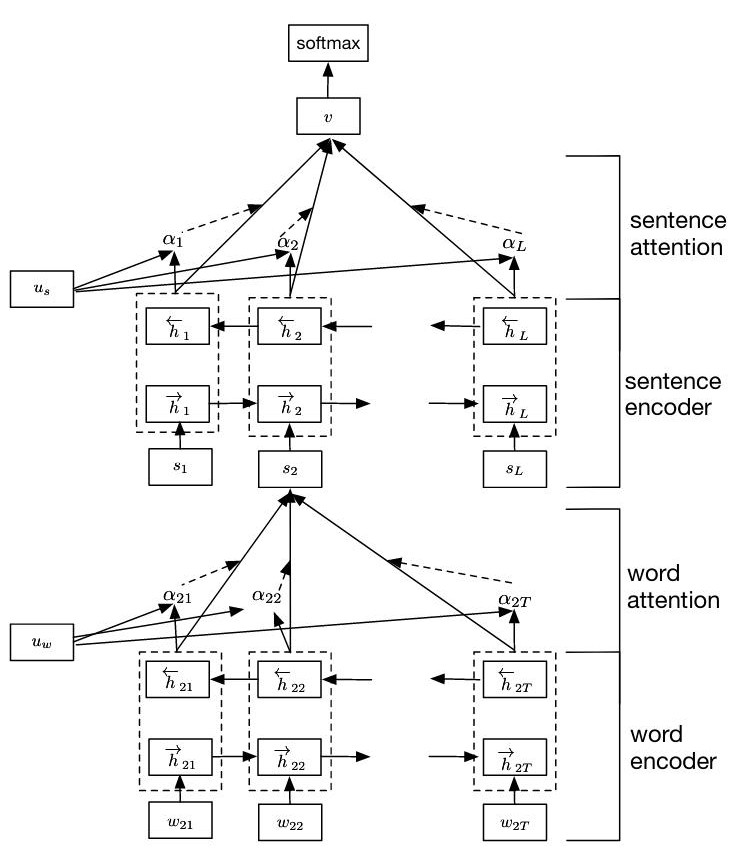
\includegraphics[width=0.8\textwidth]{HAN}
    \caption{شبکه‌ی HAN}
    \label{fig:HAN}
\end{figure}

در این شبکه در ابتدا کلمات به نمایش‌های برداری
رمزنگاری\footnote{Encode}
می‌شوند. برای این کار از مدل
GRU
دو طرفه\footnote{\lr{Bidirectional GRU}}
استفاده می‌شود. در نهایت نمایش برداری کلمه ترکیب 
بخش پنهان پیش رفته\footnote{\lr{Forward Hidden State}}
و 
بخش پنهان بازگشتی\footnote{\lr{Backward Hidden State}}
است. اما تمام این کلمات ارزش یکسانی ندارند، در واقع برای نمایش و به دست آوردن معنای جمله، نمی‌توان و نباید
از تمام کلمات تشکیل دهنده‌ی آن به یک اندازه استفاده نمود. به همین دلیل در لایه‌ی بعدی از مکانیزم توجه
استفاده شده‌است. نتایج به دست آمده یه یک شبکه
MLP\footnote{\lr{Multilaye Perceptron}}
با تابع فعال‌ساز سافت‌مکس داده می‌شود تا به یک مقدار تکی دست یافت.

نتایج لایه‌ی قبل، از کلمات نمایش سطح  جمله را تشکیل می‌دهند.
به مانند سطح کلمه در سطح جمله نیز از یک شبکه دو طرفه
GRU
برای رمزنگاری استفاده شده‌است و بردار نمایش آن ترکیبی از حالت جلو رونده و عقب رونده است.
حال برای آن که مشخص شود کدام جملات به رسیدن به دقت بالاتر در حل مسئله‌ی یافتن
کلاس مناسب بیشتر کمک می‌کنند، باز هم ار یک لایه مکانیزم توجه استفاده شده‌است. نتیجه این
قسمت نیز برداری مرتبط با جملات متن است. مجموع این بردار‌ها، بردار سند اصلی را تشکیل می‌دهند
که یک نمایش سطح بالا از سند است. این بردار ورودی تابع سافت‌مکس می‌شود تا کلاس تخمین زده شود.

در این مقاله از دو روش
pooling
نیز استفاده شده تا به جای مکانیزم توجه استفاده شوند و نتایج مقایسه شد. 
دو روش
میانگین\footnote{\lr{Average Pooling}}
و
بیشترین\footnote{\lr{Max Pooling}}
در مقایسه با مکانیزم توجه دقت کمتری در تمام موارد داشتند که نشان دهنده‌ی عملکرد خوب مکانیزم توجه در این موارد است.

\subsubsection{VDCNN}

شبکه‌های استفاده شده در امور پردازش زبان و گفتار طبیعی اغلب از خانواده
RNN
ها به خصوص
LSTM
و
CNN
ها هستند. اما این شبکه‌ها در مقابل شبکه‌هایی که در مسائل مربوط به 
بینایی ماشین\footnote{\lr{Machine Vision}}
استفاده شده‌اند عمق کمتری دارند.

در
\cite{conneau2016very}
شبکه‌ای با ساختار جدید ارائه شده‌است که عملیات را به طور مستقیم در سطح حروف بر روی متون انجام می‌دهد
و تنها از کانولوشن‌های کوچک و عملیات‌های
pooling
استفاده می‌کند. هدف از این مقاله آن است که بتوان با افزایش لایه‌ها دقت مدل را بالا برد و به عملکرد بهتری
دست یافت، به همین دلیل نیز مدل
شبکه عصبی کانولوشنی بسیار عمیق\footnote{\lr{Very Deep Convolutional Neural Network}}
نام گذاری شده‌است.
با افزایش تعداد لایه‌های کانولوشنی به ۲۹ عدد این مدل در تعدادی از مسائل عملکرد بهتری از
رقبا نشان می‌دهد.

در ابتدا حروف تشکیل دهنده‌ی متن به نمایش برداری در می‌ایند، سپس با استفاده از یک
جدول مراجعه\footnote{\lr{Look-up Table}}
این نمایش‌ها را به یک
تنسور\footnote{\lr{Tensor}}
دو بعدی تبدیل می‌کند. در مرحله بعدی یک لایه کانولوشنی با اندازه ۳ و تعداد ۶۴ وجود دارد. بعد از این
لایه تعدادی لایه کانولوشنی دیگر می‌آید. در این شبکه با الهام از
VGG
و
ResNets
دو قانون تعریف شده‌است:

\begin{enumerate}
    \item برای لایه‌هایی با ابعاد ورودی یکسان بردار ویژگی\footnote{\lr{Feature Map}} اندازه یکسانی دارد.
    \item اگر ابعاد ورودی نصف شود، بردار ویژگی دو برابر می‌شود.
\end{enumerate}

شبکه از ۳ لایه‌ی
pooling
تشکیل شده‌است که هر کدام ورودی لایه‌ی بعدی را نصف لایه‌ی قبل می‌کنند. در واقع این سبب می‌شود که ابعاد
بردار ویژگی ثابت باشد مگر بعد از لایه‌ی
pooling
که سبب نصف شدن ورودی و با توجه به قانون‌های گفته شده، دو برابر شدن اندازه بردار ویژگی می‌شود.
با این تفاسیر و شروع با ۶۴ کانولوشن، بعد از
pooling
اول به ۱۲۸ و سپس به ۲۵۶ و در لایه‌ی آخر به ۵۱۲ کانولوشن می‌رسیم.

در این شبکه از ایده‌ی
n-Grams
برای ساخت مدل استفاده شده‌است. به همین دلیل از تعداد زیادی کانولوشن اما با ابعاد کوچک استفاده شده است.
همچنین با الهام از شبکه‌ی
ResNet
میانبر‌هایی\footnote{\lr{Shortcuts}}
در مدل وجود دارند.

\subsection{بررسی چند مقاله}

برای انجام عمل دسته بندی در متون در سطوح مختلف جمله، کلمه و حروف تلاش‌های زیادی انجام شد.
\cite{graves2005framewise}
در سال ۲۰۰۵ نشان داد که استفاده از شبکه‌های
\lr{Bidirectional LSTM}
می‌تواند نتایجی بهتر از مدل‌های
RNN
معمولی به دست آورد. برای این کار در لایه‌های پنهان مدل ارتباطات دو طرفه اضافه کردند و با بررسی نتایج مهر تعییدی
بر عملکرد بهتر شبکه‌ی بر پایه‌ی حافظه‌ی دوطرفه زدند.

در
\cite{liu2016recurrent}
مدلی برای ذخیره سازی موقت ارتباطات معنایی جملات بلند معرفی شد. در شبکه که از
LSTM
استفاده شده‌است کلمات را به صورت تک تک بررسی می‌کند این مسئله سبب می‌شود که مدل از نظر درک
معانی از عملکرد و بهینگی بهتر و بالاتری برخوردار باشد.

در
\cite{dieng2016topicrnn}
مدل
TopicRNN
معرفی شد که هدف آن کلاس بندی با در نظر گرفتن وابستگی‌های متن است.
در این روش با استفاده از
مدل عناوین پنهان\footnote{\lr{Latent Topic Models}}
وابستگی‌های معنایی
جهانی\footnote{\lr{Global}}
استخراج می‌شوند تا بخش اصلی مدل یعنی شبکه‌ی
RNN
بتواند فقط به استخراج وابستگی‌های
محلی\footnote{\lr{Local}}
تمرکز کند.

ایان گوفلو\footnote{\lr{Ian J Goodfellow}}
شخصی است که تاثیر زیادی در علم هوش مصنوعی داشته‌است. یکی از دستاورد‌های او معرفی
مثال‌های خصومتی\footnote{\lr{Adversarial examples}}
است.
یادگیری خصومتی\footnote{\lr{Adversarial training}}
که توسط گودفلو ارائه شده‌است، در
\cite{miyato2017adversarial}
استفاده می‌شود تا علاوه بر بالا بردن دقت از
بیش‌برازش\footnote{\lr{Overfitting}}
جلوگیری شود. این مقاله در سطح کلمه به حل مسئله می‌پردازد.

مقاله‌ی
\cite{guggilla-etal-2016-cnn}
نیز به مانند 
\cite{wang-etal-2016-combination}
از ترکیب دو شبکه‌ی
CNN
و
LSTM
برای ساخت مدل خود استفاده کرد. این مدل با بهره گیری از روش نمایش
Word2Vec
به این عمل پرداخت. هر دو شبکه‌ی کانولوشنان و دارای حافظه استفاده‌های زیادی در مسائل طبقه بندی داشته‌اند و ترکیب آن‌ها
نیز نتایج خوبی را ارائه داده است.

شبکه‌های عمیق معمولا نتایج بهتری با توجه به پیچیدگی مدل و روابط متون و اجزای تشکیل دهنده‌ی آن داردند.
اما سبب افزایش چشم‌گیر پیچیدگی مدل و هزینه‌ی محاسباتی ان می‌شود.
در
\cite{johnson-zhang-2017-deep}
شبکه
DPCNN
معرفی شد تا این مشکل را حل کند. نسبت به
ResNet
این شبکه از پیچیدگی کمتری برای انتخاب این که میانبرها در چه مکانی به کار گرفته شوند استفاده می‌کند.

روش‌های محتلفی بر پایه‌ی
Transformer
ها ارائه شده‌اند. از میان این روش‌ها روش
BERT
به دلیل کاربرد بسیار و همچنین ارائه به عنوان اولین مدل موفق از نوع خود از اهمیت بالایی برخوردار است که به بررسی آن
پرداخته شد. شبکه‌های بسیاری برای بالا بردن دقت از
BERT
استفاده کرده‌اند. به طور کل در میان مقالاتی که از
Transformer
ها برای حل مسائل پردازش زبان طبیعی استفاده کرده‌اند، شبکه‌ی
BERT
جایگاه ویژه‌ای دارد.
\cite{schmidt2020data}
از سه مدل
BERT
استفاده شده‌است،
BERT-base
، مدل چندزبانه
BERT
و در آخر
SCIBERT
.
در این مدل لایه‌ی مربوط به
classification
در مدل اصلی با لایه‌ای متفا.ت جایگذاری شده‌است. این لایه همچنان خطی و
به طور کامل متصل\footnote{Fully-connected}
است، اما به جای خطای
\lr{sigmoid cross-entropy}
از
\lr{logits function}
استفاده شده‌است. این کار سبب شده‌است که مدل قادر به تخمین زدن به صورت چند کلاسه نیز باشد.

\section{روش‌های بر پایه رویکرد تحلیل عواطف و احساسات}

تحقیقات انجام شده روش‌های گوناگون و زیادی را برای انجام این فعالیت ارائه داده‌اند که شامل هر دو روش
نظارت شده و نظارت نشده می‌شوند.
در این تحقیقات انواع و اقسام روش‌های نظارت شده به منظور استخراج اطلاعات از نظرات کاربران
استفاده شده‌اند که می‌توان از میان آن‌ها به
\lr{Support	Vector	Machines (SVM)}
،
\lr{Maximum Entropy}
و
\lr{Naïve Bayes}
اشاره کرد.
روش‌های نظارت نشده نیز دستاورد‌های زیادی داشته‌اند.

از حدود یک دهه گذشته روش‌های مبتنی بر یادگیری عمیق پر قدرت وارد این عرصه شدند و نتایج پیشرفته‌ای
از خود در زمینه پردازش زبان و گفتار طبیعی به خصوص
\lr{Sentiment analysis}
به جای گذاشتند.
همین مسئله سبب افزایش استفاده از یادگیری عمیق در مسائل مربوط به استخراج اطلاعات و تجزیه تحلیل
عواطف و احساسات شد.
\cite{zhang2018deep}


\subsubsection{وابستگی به هدف}
در بحث استخراج و تحلیل عواطف و احساسات از متون موردی که تاثیر بسیاری در نتیجه‌ی نهایی دارد هدف یا به اصطلاح
target
می‌باشد. به عنوان مثال جمله‌ی زیر با توجه به این که هدف بررسی، سیستم عامل ویندوز باشد یا لینوکس نتیجه‌ی متفاوتی دارد.
\begin{quotation}
    لینوکس عملکرد بهتری نسبت به ویندوز دارد.
\end{quotation}
اگر هدف ما کلمه‌ی لینوکس باشد نتیجه‌ی استخراج و تحلیل متن مثبت می‌شود، و اگر هدف ویندوز باشد، نتیجه منفی است.
در صورت آن که هدف کلمه‌ی دیگری مثل اندروید باشد، نتیجه‌ی خنثی حاصل می‌شود.

مقاله‌ی
\cite{68dong-etal-2014-adaptive}
با ارائه
AdaRNN
متون را با وابستگی به هدف مورد بررسی قرار داد. این مدل با یادگیری آن که کلمه یا کلمات حاوی اطلاعات مهم را با
ربط دادن به کلمه‌ی هدف استخراج کند، متون را از دید ساختاری بررسی می‌کند.

شبکه
LSTM
می‌تواند ارتباطات معنایی بین کلمه‌ یا کلمات هدف و جملات را به دست آورد. در
\cite{70tang-etal-2016-effective}
با استفاده از این ویژگی
LSTM
دو شبکه
TD-LSTM\footnote{\lr{Target-Dependent LSTM}}
و
TC-LSTM\footnote{\lr{Target-connection LSTM}}
ارائه شد. برای این کار کلمه‌ی هدف را به عنوان یک ویژگی به شبکه‌های ایجاد شده اضافه کردند.
شبکه‌های
LSTM
قادر به درک ارتباطات معنایی درون ساختاری هستند و در فهم و پردازش ارتباطات بین جملات به خوبی عمل نمی‌کنند.
به عنوان مثال این شبکه‌ها می‌توانند پیش‌زمینه جمله را درک کنند، در جملات کیفیت غذای این رستوران بسیار بالاست.
من عاشق این رستوران هستم. کیفیت غذا پیش‌زمینه‌ی جمله‌ی مثبت بعدی است. اما پیچیدگی کنار هم
قرار گرفتن جملات مفهومی نیست که به راحتی درک شود.

در
\cite{71ruder-etal-2016-hierarchical}
مقاله با استفاده از یک شبکه حافظه بلند کوتاه مدت سلسله مراتبی دو طرفه\footnote{\lr{Hierarchical bidirectional long short-term memory}}
به شناخت و درک هر دو نوع ارتباط گفته شده پرداخته شده‌است. به دلیل وجود وابستگی مدل تنها به جمله و
ساختار آن، این شبکه را قادر به انجام پیشبینی در زبان‌های مختلف می‌سازد.

این مدل از ۳ بخش مختلف تشکیل شده‌است. بخش اول تبدیل به نمایش برداری است. هر نظری کاربران در سطح شبکه‌های
اجتماعی یا دیگر سکوهای\footnote{Platforms}
موجود ارسال می‌کنند از چند جمله تشکیل شده‌است. این جملات با استفاده از لایه گذاری\footnote{Padding}
به طول یکسان تبدیل می‌شوند. سپس هر جمله تبدیل به نمایشی از مجموعه بردارهای کلمات تشکیل دهنده آن می‌شود.
سپس هر کدام از جملات با کلمه‌ی مورد نظر و ویژگی آن (به عنوان مثال غذا\#کیفیت)
ترکیب می‌شود. به این شکل که از این دو کلمه میانگین گرفته می‌شود و به بردار اضافه می‌شود.

بخش بعدی شبکه‌ی
LSTM
است که امکان یادگیری وابستگی‌های جملات را دارد. دو شبکه‌ در ساختار وجود دارند که یکی از آن‌ها
رو به جلو است و دیگری رو به عقب.

بخش بعدی شامل دو شبکه‌ی
LSTM
دیگر است که به مانند قسمت قبل یکی رو به جلو است و دیگری رو به عقب. این دو شبکه از خروجی بخش قبلی
استفاده می‌کنند و جملات را به طور کلی و در سطح متن بررسی می‌کنند.

\begin{table}[!ht]
    \begin{small}
    \begin{center}
      \begin{latin}
      \begin{tabular}{|l|l|l|l|l|l|}
        \hline
        Language & Domain & Best & LSTM & H-LSTM &  HP-LSTM \\
        \hline
        English & Restaurants & 88.1 & 81.4 & 83.0 & 85.3 \\
        \hline
        Spanish & Restaurants & 83.6 & 75.7 & 79.5 & 81.8 \\
        \hline
        French & Restaurants & 78.8 & 69.8 & 73.6 & 75.4 \\
        \hline
        Russian & Restaurants & 77.9 & 73.9 & 78.1 & 77.4 \\
        \hline
        Dutch & Restaurants & 77.8 & 73.6 & 82.2 & 84.8 \\
        \hline
        Turkish & Restaurants & 84.3 & 73.6 & 76.7 & 79.2 \\
        \hline
        Arabic & Hotels & 82.7 & 80.5 & 82.8 & 82.9 \\
        \hline
        English & Laptops & 82.8 & 76.0 & 77.4 & 80.1 \\
        \hline
        Dutch & Phones & 83.3 & 81.8 & 81.3 & 83.6 \\
        \hline
        Chinese & Cameras & 80.5 & 77.6 & 78.6 & 78.8 \\
        \hline
        Chinese & Phones & 73.3 & 70.3 & 74.1 & 73.3 \\
        \hline
      \end{tabular}
      \end{latin}
      \caption{مقایسه عملکرد مدل معرفی شده با شبکه‌های دیگر}
      \label{tab:H-LSTM}
    \end{center}
\end{small}
  \end{table}

در همین راستا در
\cite{72Zhang_Zhang_Vo_2016}
شبکه‌ای در سطح جمله ارائه شد که هدف آن رفع مشکل و ضعف استفاده از
pooling
است. برای این کار از دو
GRU\footnote{\lr{Gated Recurrent Uunit}}
استفاده شده‌است. در ابتدا یک
GRU
دو طرفه\footnote{\lr{Bidirectional Gated Recurrent Uunit}}
ایجاد شده که هدف آن پردازش کلمات متن است تا
pooling
به جای آن که مستقیم بر کلمات تاثیر بگذارد به خروجی این لایه اعمال شود. سپس از یک
GRU
سه طرفه استفاده شده تا ارتباطات میان کلمه‌ی هدف و کلمات اطراف آن را درک کند.
این شبکه سه طرفه برا آن اضافه شده‌است تا بتواند ارتباطات معنایی و ساختاری متون را مدل سازی کند.
این مقاله نشان داد که استفاده از
GRU
سبب کم شدن جانب‌داری\footnote{bias}
در تصمیم گیری‌های مدل می‌شود.

در
\cite{74YANGATT}
دو شبکه
LSTM
بر پایه مکانیزم توجه ارائه شد با هدف این که مدلشان سبب افزایش دقت کلاس بندی\footnote{Classification}
شود.

در مدل اول
(\lr{AB-LSTM1})
وزن‌های به دست آمده در لایه‌ی پنهان یعنی نتیجه‌ی
LSTM
با نمایش برداری وزن‌های به دست آمده از هدف و جنبه‌ی بررسی ضرب می‌شوند و به شبکه
مکانیزم توجه داده می‌شوند.

مدل دوم 
(\lr{AB-LSTM2})
این وزن‌ها با فرمول 
\ref{formula:AB-LSTM2}
با هم ترکیب می‌شوند و به مکانیزم توجه داده می‌شوند.

\begin{equation}
    a_t=softmax(h_t^TW_bh_{target})
\end{equation}
\begin{equation}
    o={\Sigma_{t=1}^T a_th_t }
    \label{formula:AB-LSTM2}
\end{equation}

در
\cite{79ma2017interactive}
مدل
IAN\footnote{\lr{Interactive Attention Network}}
ارائه شده که توجه آن هم به جنبه و هم به متن نوشته است.
در این مقاله از دو شبکه بر پایه مکانیزم توجه استفاده شده‌است تا به صورت تعاملی کلمات مهم هدف و کلمات مهم
کل متن را دریابد.


\paragraph{ATAE-LSTM} \hfill \break

همنطور که گفته شد، شبکه‌ی
LSTM
قادر به درک روابط معنایی و ساختاری در جملات است که مقاله‌های متعددی از این شبکه و ویژگی‌های آن برای
ساخت مدل‌هایی با قابلیت تحلیل عواطف و احساسات با توجه به کلمه‌ی هدف پرداختند. اما نکته‌ای که وجود دارد آن است
که این شبکه‌ها قادر به تشخیص آن که کدام بخش از جمله اهمیت بالاتری دارد، نیستند.

در
\cite{73wang-etal-2016-attention}
برای رفع این کاستی و یافتن نقاط مهم جمله با توجه به کلمه ی هدف\footnote{Target}
از مکانیزم توجه\footnote{\lr{Attention Mechanism}}
بهره گیری شده‌است. در این مقاله سه مدل
AE-LSTM\footnote{\lr{LSTM with Aspect Embedding}}
،
AT-LSTM\footnote{\lr{Attention-based LSTM}}
و
ATAE-LSTM\footnote{\lr{Attention-based LSTM with AspectEmbeddin}}
که ترکیب دو روش قبلی است معرفی شده‌است.

در روش
AE-LSTM
بردار
embedding
جنبه و هدف\footnote{Aspect}
یادگیری می‌شود.

در روش
AT-LSTM
معماری مدل طوری چیده شده‌است تا جنبه و هدف مورد تحلیل بر وزن‌های بخش مکانیزم توجه تاثیر بگذارند. برای این
کار بردار مربوط به کلمه یا کلمات هدف را به نتیجه‌ی خروجی از لایه‌ی
LSTM
اضافه می‌کنند و به بخش مکانیزم توجه می‌دهند. مکانیزم توجه به مدل اجازه می‌دهد تا بخش‌های مهم جمله را
با توجه به جنبه و هدف‌های مختلفی که به آن داده شده‌است، بیابد.

روش
ATAE-LSTM
که ترکیبی از دو روش قبلی است، از اطلاعات به دست آمده از
AE-LSTM
استفاده می‌کند، اما برای این که این اطلاعات تاثیر بیشتری روی مدل بگذارند و بهتر بررسی شوند علاوه بر
اضافه کردن به خروجی لایه‌ی
LSTM
آن را به نمایش برداری جمله اضافه می‌کند. ساختار این شبکه در تصویر
\ref{fig:ATAE-LSTM}
آمده است.

\begin{figure}[!ht]
    \centering
    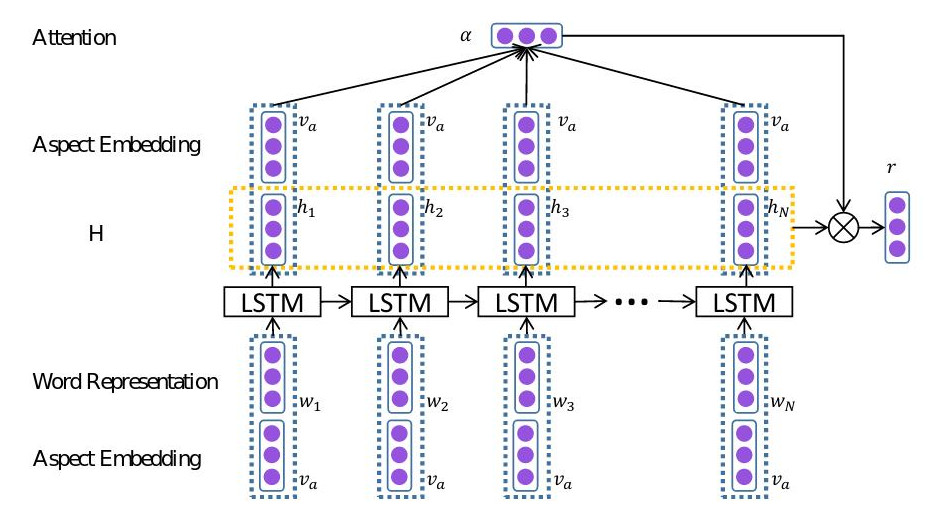
\includegraphics[width=0.8\textwidth]{ATAE-LSTM}
    \caption{ ساختار شبکه‌ی 
        ATAE-LSTM -
        در این تصویر ناحیه‌ی مشخص شده با رنگ زرد خروجی لایه‌ی حافظه کوتاه مدت بلند است.
        بردار نمایش جنبه و هدف، به این لایه اضافه شده‌است که به مانند ساختار
        AT-LSTM
        می‌باشد. این بردار به نمایش برداری کلمات جمله نیز اضافه شده‌است که با این کار شبکه به
        ATAE-LSTM
        تبدیل می‌شود.
    }
    \label{fig:ATAE-LSTM}
\end{figure}

هیتمپ کلمات مهم و پر اهمیت با توجه به هدف و جنبه‌ی مشخص شده در تصویر
\ref{fig:ATAE-HM}
آمده‌است.

\begin{figure}[!ht]
    \centering
    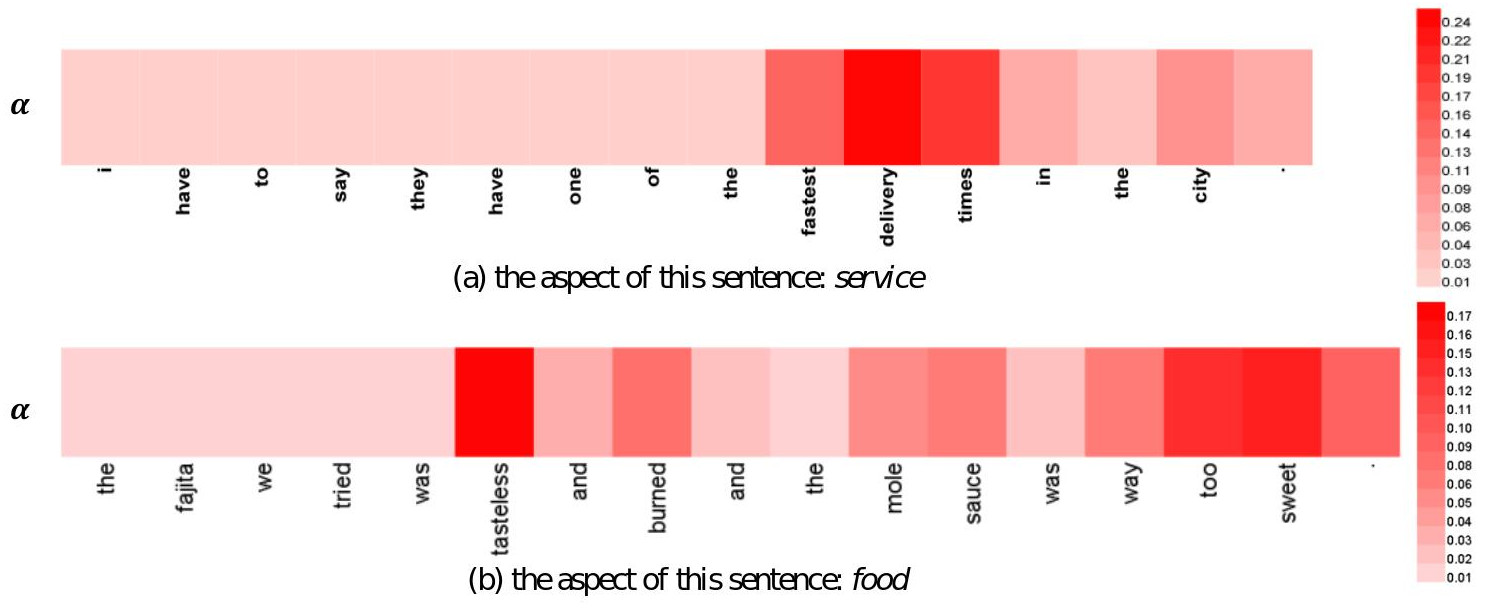
\includegraphics[width=1\textwidth]{ATAE-HM}
    \caption{ هیتمپ کلمات مهم جمله }
    \label{fig:ATAE-HM}
\end{figure}

\paragraph{MemNet} \hfill \break

شبکه‌های
LSTM
علارقم استفاده‌ی زیادی که در زمینه تحلیل احساسات و درک محتوای متون دارند، از نظر زمان آموزش بسیار کند هستند.
این نوع شبکه‌ها به دلیل ساختاری که دارند علاوه بر آن که نمی‌توان آن‌ها را به شکل 
موازی\footnote{Paraller}
یادگیری کرد، زمان یادگیری نیز نسبت به دیگر مدل‌ها بالاتر است.

در
\cite{76tang2016aspect}
با ارائه یک شبکه عمیق بر اساس
MemmNN\footnote{\lr{Memmory Nueral Network}}
ها این مشکل را حل کردند. علاوه بر این مسئله، شبکه‌های بر پایه حافظه نتیجه گیری را بر اساس قطبیت جنبه
و هدف مورد نظر در جمله انجام می‌دهند. روش ارائه شده بر مبنای داده کار می‌کند و نیازی به تجزیه کننده جمله یا
فرهنگ لغت عواطف و احساسات ندارد. همجنین ساختار مدل ارائه شده به طوری است که از نظر محاسباتی نیز کم هزینه باشد.

شبکه از چند لایه‌ی محاسباتی همراه 
پپارامتر‌های اشتراکی\footnote{\lr{Shared parameters}}
تشکبل شده‌است. هر لایه یک یک مدل بر پایه
توجه\footnote{Attention}
است. هر کدام از این مدل‌ها در ابتدا یاد می‌گیرند که کدام یک از مفاهیم کلمات درون جمله با توجه به
جنبه‌ی\footnote{Aspect}
مورد نظر از اهمیت بالاتری برخوردار هستند و سپس نمایشی از متن را یادگیری می‌کنند.
این نمایش به دست آمده از آخرین لایه از مدل‌های بر اساس توجه به عنوان ورودی برای تحلیل عواطف و احساسات
متن استفاده می‌شوند. با توجه به
end-to-end
بودن ساختار شبکه می‌توان این مدل را با استفاده از 
\lr{gradient descent}
و با استفاده از
تابع خطای\footnote{Loss Function}
cross-entropy
یادگیری کرد.

برای این کار هر کلمه ی ورودی به
embedding
تبدیل می‌شود. کلمه‌ی هدف نیز همراه با کلمات
embed
می‌شود، اگر تک کلمه‌ای باشد به صورت مستقیم این اتفاق رخ می‌دهد و اگر جند کلمه‌ای باشد میانگین نمایش
آن محاسبه می‌شود. همان طور که گفته شد این مدل از تعدادی لایه تشمیل شده‌است. که هر لایه شامل یک
بخش توجه و یک بخش خطی است.
بردار نمایش ساخته شده از کلمات به لایه‌ی اول داده می‌شوند، بخش
attention
مدارک مهم مورد نیاز را از حافظه دریافت می‌کند، خروجی این بخش و بخش خطی با یکدیگر جمع می‌شوند
و به لایه‌ی بعد داده می‌شوند. این کار تکرار می‌شود تا ویژگی‌های پیچیده و درونی بیشتری استخراج شوند. خروجی
لایه‌ی اخر به یک تابع سافت‌مکس داده می‌شود تا نتیجه نهایی تولید شود.


\subsubsection{طول متن}

طول متون نیز اهمیت بالایی در نتیجه گیری بر اساس متن‌ها و دریافت عواطف و احساسات دارد.
در متون کوتاه مثل توییت‌ها یا تک جمله‌ها، به دلیل عدم وجود اطلاعات زیاد به دست آوردن تخمین درستی از
عواطف و احساسات قرار گرفته در مفاهیم متن کاری بسیار دشوار است.
برای این کار لازم است تا علوه بر داشتن دانش قبلی از استراتژی‌ها به خصوصی استفاده نمود.

\paragraph{CharSCNN} \hfill \break

در
\cite{dos2014deep}
با به کار گیری از یک شبکه‌ی عمیق کانولوشنی با نام
CharSCNN
این مشکل را حل کردند. برای این کار ابتدا کلمات متن را به صورت برداری تبدیل می‌کنند در واقع عملیات
embedding
انجام می‌شود. سپس هر بردار به دو بردار تبدیل می‌شود. یکی بردار در سطح کلمات و دیگری بردار در سطح حروف.

\begin{figure}[!ht]
    \centering
    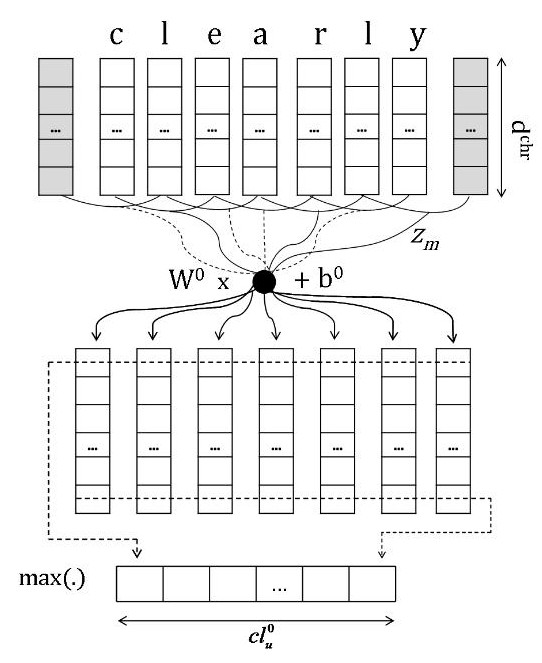
\includegraphics[width=0.5\textwidth]{CHARCNN}
    \caption{ شبکه‌ی کانولوشنی در سطح حروف }
    \label{fig:CHARCNN}
\end{figure}

در مرحله‌ی بعدی نمایش جمله‌ای از متن با استفاده از یک شبکه‌های کانولوشنی دیگر به دست می‌آید.
چالش اصلی این بخش آن است که طول جملات ثابت نیستند و قسمت‌های مهم جمله و نمایانگر عواطف و احساسات
ممکن است در هر نقطه از جمله وجود داشته باشند. این لایه، در واقع شبکه‌ی کانولوشنی است که وظیفه‌ی آن
به دست آوردن این نمایش از متن است. این کار با به دست آوردن ویژگی‌های محلی اطراف هر کلمه و ترکیب
آن‌ها با استفاده ماکزیمم گیری انجام می‌شود.

\subsection{بررسی چند مقاله}

در سال ۲۰۱۳ در مقاله
\cite{Moraes2013DocumentlevelSC}
مقایسه‌ای بین
SVM\footnote{\lr{Support Vector Machines}}
و
ANN\footnote{\lr{Artificial Neural Networks}}
برای طبقه بندی متون در سطح سند انجام شد. این مقایسه نشان داد که شبکه‌‌های عصبی عمیق می‌توانند نتایجی نزدیک به
SVM
را به دست آورند. در بسیاری از موارد نتایج به دست آمده قابلیت رقابت با عملکرد‌
SVM
را دارا هستند. این مسئله سبب آن شد که بسیاری با استناد به مقاله‌ی معرفی شده سعی در حل چالش‌های پردازش زبان و متن کاوی
با استفاده از شبکه‌های عمیق دارند.

در
\cite{xu2016cached}
مدلی به عنوان
cached-LSTM
معرفی شد تا بتواند ارتباطات معنایی در متون بلند را درک کند. این مدل تشکیل شده از چند بخش است که هر یک از این
بخش‌ها میزان فراموشی مربوط به خود را داردند. این کار سبب می‌شود تا بخش‌هایی از حافظه با میزان فراموشی کم‌تر ویژگی‌های
معنایی
global
یک متن را استخراج کنند و بخش‌های با میزان فراموشی بالا به ارتباطات و ویژگی‌های معنایی
local
دست یابند.

مقالات زیادی سعی بر استفاده و کمک گرفتن از جنبه‌های دیگر برای حل مسئله‌ی تحلیل عواطف و احساسات دارند،
به عنوان مثال مقاله‌ی
\cite{yin-etal-2017-document}
به این عمل از دید مسئله‌ی درک ماشین نگاه می‌کند و با ارائه یک مدل سلسله مراتبی بر اساس
attention
و معماری شبکه‌ی
LSTM
این مسئله را حل می‌کند.
در همین راستا مقاله
\cite{zhou-etal-2016-attention}
با کمک گرفتن از زبان انگلیسی که داده‌ها و منابع زیادی برای انجام عمل یادگیری برای آن وجود دارد، تحلیل
عواطف را در زبان‌های دیگر که دیتاست‌های کمتری برای آن‌ها موجود است انجام می‌دهد. این کار با استفاده از دو شبکه
LSTM
بر اساس
attention
که ساختاری سلسله مراتبی دارند انجام می‌شود.
در
\cite{ijcai2017-311}
نیز با استفده از
MemNN
و
یادگیری انتقالی\footnote{\lr{transfer learning}}
به تحلیل عواطف و احساسات در سطح سند پرداخته می‌شود.
\cite{teng-etal-2016-context}
نیز با ارائه‌ی مدل
\lr{Bidirectional LSTM}
حساس به متن، با استفاده از دایره لغاتی از کلمات حاوی اطلاعات احساسی با وزن‌های متفاوت روشی برای حل این مسئله ارائه داد.

همانطور که گفته شد متون کوتاه چالش‌های اضافه‌ای به دلیل نبود اطلاعات کافی معنایی برای تشخیص و دسته بندی عواطف
و احساسات درون متن دارند.
\cite{wang-etal-2016-combination}
با دانش بر این مسئله که شبکه‌های کانولوشنال درک خوبی از قرار گیری کلمات در کنار یکدیگر دارند و همچنین دقت
بهتر شبکه‌های
RNN
در حل اینگونه مسائل با ترکیب کردن این دو شبکه، مدلی برای امر تحلیل و بررسی عواطف و احساسات ارائه داد.

بازارهای مالی یکی از جذاب‌ترین موارد برای تحقیق در زمینه پردازش زبان طبیعی هستند زیرا اطلاعات زیادی از قبیل
توییت‌های افراد و همچنین کارشناسان این زمینه به طور مداوم در حال ایجاد شدن است. مقاله‌های بسیاری به طور خاص در زمینه
پردازش متون مربوط به بازارهای مالی و استخراج عواطف و احساسات و در نهایت نتیجه گیری از آن‌ها ارائه شده‌اند که
\cite{akhtar2017multilayer}
یکی از آن‌ها است. در این مقاله با ایجاد شبکه‌ای با ساختاری شبیه به
\lr{Multilayer Perceptron}
که در تصویر
\ref{fig:MLP-ensemble}
آورده شده‌است، به تحلیل متون مربوط به بازار‌های مالی پرداخته است.

\begin{figure}[!ht]
    \centering
    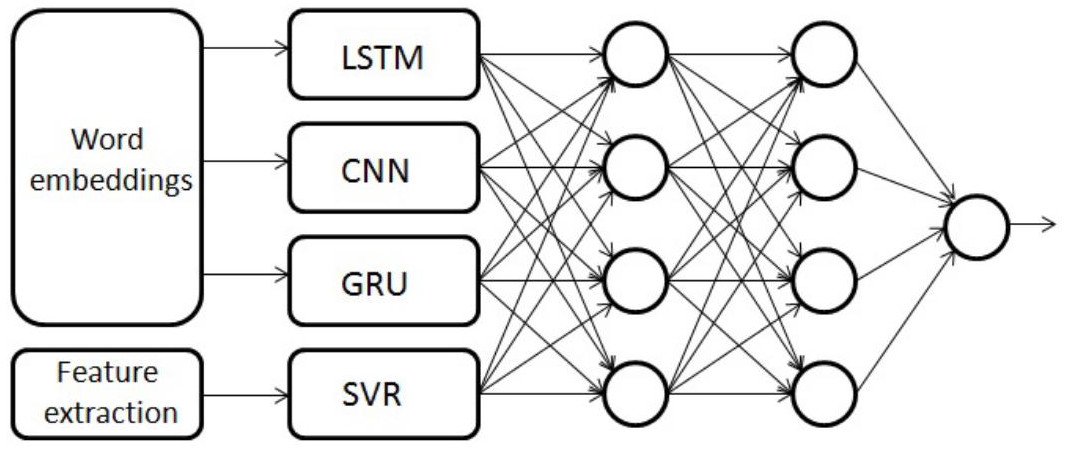
\includegraphics[width=0.8\textwidth]{MLPENSEMBLE}
    \caption{ ترکیب بر اساس MLP }
    \label{fig:MLP-ensemble}
\end{figure}

در این شبکه از نتایج شبکه‌های
LSTM
،
CNN
و 
GRU
استفاده شده‌است و با اضافه کردن تعدادی لایه‌ی
fully-connected
نتیجه‌ی نهایی ایجاد می‌شود.

\section{روش‌های بر پایه رویکرد ترجمه ماشینی}

\subsubsection{یادگیری دنباله به دنباله}
شبکه های عصبی در حل بسیاری از موارد سخت عملکرد مناسبی از خود نشان داده‌اند اما هیچ مدلی برای رسیدن از
یک دنباله به دنباله‌ای دیگر  در تحلیل متن طراحی نشده بود، البته تا قبل از
\cite{sutskever2014sequence}.
دنباله‌ها برای شبکه‌های عصبی چال‌های یزرگی هستند زیرا برای پردازش آن‌ها نیاز است تا طول ثابت داشته باشند اما
هیچ گاه نمی‌توان تضمین کرد که دنباله‌های موجود طول یکسان دارند. در واقع
یادگیری دنباله به دنباله\footnote{\lr{Sequence to Sequence Learning}}
کاری بسیار دشوار است. در این مقاله از شبکه‌های
LSTM
استفاده شده‌است تا به تحلیل این نوع از مسائل بپردازند.

دو شبکه‌ی
LSTM
استفاده شده‌است که یکی برای دریافت دنباله و خواندن اطلاعات در واحد زمان و به طور تک تک تا بتوان یک
نمایش برداری از دنباله دست یافت و دیگری برای استخراج خروجی از نمایش برداری ایجاد شده.
دلیل استفاده از
LSTM
قابلیت آن برای دست‌یابی و یادگیری وابستگی‌های موقت و با فاصله است.

در این مقاله بررسی شده‌است که استفاده از
RNN
ها برای حل مشکل تبدیل دنباله به 
فضای برداری با ابعاد ثابت
و همچنین تبدیل نمایش برداری به دنباله نهایی قابل استفاده هستند. اما مشکل وجود وابستگی‌های بین کلمات و متون در
فواصل بلند است. به همین دلیل از
LSTM
که قابلیت درک این موارد را دارد استفاده شده‌است.

نکته‌ی دیگر این مقاله موازی سازی یادگیری
LSTM
است. برای این کار از ۸
واحد پردازنده گرافیکی\footnote{\lr{Graphical Processing Unit (GPU)}}
استفاده شده‌است. این مدل دارای دو شبکه
LSTM
است که هر کدام ۴ لایه دارند. در واقع برای موازی سازی هر کدام از لایه‌ها در یکی از
GPU
ها قرار می‌گیردن و وقتی خروجی لایه‌ی قبل آماده شد فرایند یاد گیری در لایه‌ی کنونی شروع می‌شود.
در واقع هر واحد باید صبر کند تا فرایند واحد بعدی تمام شود تا داده را به لایه بعدی ارسال کند و همچنین برای
دریافت ورودی نیز باید صبر کند تا فرایند لایه‌ی قبلی به پایان رسد.

\subsubsection{ترجمه ماشینی گوگل}

گوگل یکی از بزرگ‌ترین شرکت‌های نرم‌افزاری دنیا در سال ۲۰۱۶ مقاله‌ای برای سیستم ترجمه نرون ماشینی خود
ارائه داد. مقاله‌ی
\cite{wu2016googles}
شامل اطلاعات کامل از این مدل است.

ساختار این مدل شامل سه بخش کلی است. بخش
encoder
، بخش
decoder
و بخش مکانیزم توجه. بخش اول جمله‌ی ورودی را به لیستی از بردار ها تبدیل می‌کند. هر کلمه‌ی ورودی 
تشکیل یک بردار را می‌دهد. در قسمت
decoder
این بردار‌ها تک تک تبدیل به کلمات می‌شوند تا زمانی که به توکن
پایان جمله\footnote{\lr{End-of-Sentence (EOS)}}
برسد. این دو بخش توسط بک مکانیزم توجه به یکدیگر وصل شده‌اند که به رمزگشا اجازه می‌دهد تا بر بخش‌های
مختلف جمله تمرکز کند. ساختار کلی شبکه در تصویر
\ref{fig:ggl}
آمده است.

در این شبکه در بخش رمزنگار از یک شبکه
LSTM
با ۸ لایه استفاده شده‌استو به مانند مقاله‌ی قبلی برای موازی سازی فرایند یادگیری از ۸
GPU
استفاده شده‌است و هر لایه در واحد پردازشی مربوط به خود یادگیری می‌شود. لایه‌ی اول شبکه‌ی
encoder
ساختاری دو طرفه دارد که جهت برگشت از سخت افزار مشترک با لایه‌ی دوم استفاده می‌کند.

بخش رمزگشا نیز به همین ترتیب است. این بخش در ۸ پردازنده گرافیکی جدا پردازش می‌شود اما همه‌ی لایه‌های
آن به صورت یک طرفه هستند. این لایه‌ها از خرو.جی شبکه
attention
استفاده می‌کنند تا به اجزای مختلف جمله تمرکز لازم را ارائه دهند. 

\begin{figure}[!ht]
    \centering
    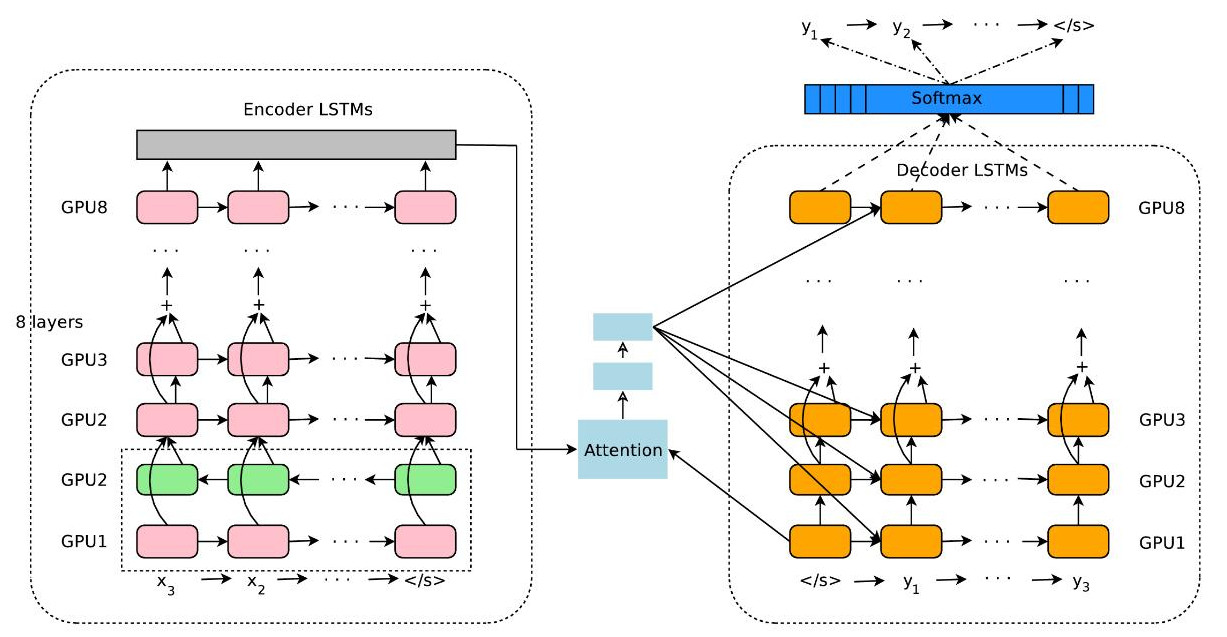
\includegraphics[width=0.8\textwidth]{ggl}
    \caption{ ساختار شبکه ترجمه گوگل }
    \label{fig:ggl}
\end{figure}

همان طور که گفته شد افزایش عمق شبکه‌ها سبب به وجود امدن
overfitting
می‌شود. برای جلوگیری از این اتفاق از
ارتباطات پسماند\footnote{\lr{residual Connections}}
استفاده شده‌است. ویژگی دیگر این مدل استفاده از یک لایه دو زرفه در بخش رمزنگار است.
در امر ترجمه اطلاعات مورد نیاز برای ترجمه‌ی یک کلمه ممکن است هر جای جمله بیایند، برای این مسئله از
ارتباطات دو طرفه در لایه اول استفاده شده‌است.

\subsection{بررسی چند مقاله}

همان طور که گفته شد اغلب روش‌های استفاده شده در این رویکرد بر پایه شبکه‌های
RNN
بنا شده‌اند. اما برخی سعی بر اضافه کردن شبکه‌های
CNN
به سبک‌های مختلف داشته‌اند. به عنوان مثال در
\cite{kalchbrenner2013recurrent}
از یک شبکه رمزنگار مبتنی بر
CNN
به همراه رمزگشای
RNN
استفاده کرد. این سبک شابد به عنوان اولین مدل‌های معرفی شده‌ی ترجمه‌ی نرونی ماشینی با به کارگیری
CNN
ها بوده است. اما این مدل از نظر عملکرد در مقابل مدل‌های مبتنی بر
RNN
ضعیف‌تر بود. اما نشان داد که می‌توان ساختار را به چه سبکی دگرگون کرد.

در سال ۲۰۱۶ محققیق
فیسبوک\footnote{\lr{Facebook}}
مدل
\cite{gehring2017convolutional}
را بر پایه
CNN
معرفی کردند که توانست در زمان خود عملکردی مشابه
RNN
ها کسب کند. مزیت استفاده از شبکه های کانولوشنال هزینه کمتر محاسباتی و سادگی مدل می‌باشد که این دو
ویژگی سبب افزایش سرعت نیز می‌شوند. یکی از روش‌های جایگزین برای
RNN
ها استفاده از
رمزنگار‌های بر پایه پولینگ\footnote{\lr{Pooling Encoders}}
است. که صرفا میانگین نمایش برداری ورودی را محاسبه می‌کنند. در این مقاله با الهام از این روش
مدلی بر پایه
CNN
ارائه شد تا اجازه دهد شبکه رمزنگاری را یادگیری کند. با
پشته کردن\footnote{\lr{Stacked}}
چند لایه به دقت مناسبی رسیدند.

در
\cite{zhou2016deep}
برای شبکه‌های
RNN
و به خصوص
LSTM
ارتباطات رو به جلوی سریع\footnote{\lr{Fast-Forward Connection}}
ایجاد شد که این مسئله سبب امکان افزایش عمق مدل‌ها بدون
overfit
شدن و با افزایش دقت مدل را فراهم کرد.

مدل‌های بر پایه
transformer
در این عمل نیز از دقت و عملکرد بالایی برخوردار هستند. برخی با تغییر دادن و بهینه سازی آن برای
عملیات مورد نظر خود، سعی در حل مسائل داشته‌اند.
\cite{bapna2018training}
یکی از آن‌ها است. در این مقاله مدل
transformer
طوری تغییر کرده‌است تا ۲ الی ۳ برابر عمیق‌تر شود. این کار سبب امکان کار با مدل‌های عمیق‌تر را می‌دهد.
در واقع مکانیزم توجه شبکه طوری تغییر داده شده‌است تا با تمام لایه‌های رمزگشا ارتباط داشته باشد. این کار شبیه
ارتباط
residual
می‌باشد که سبب افزایش انعطاف پذیری مدل جهت تعیین جریان گرادیان می‌شود.

\cite{wang2019learning}
نیز همین کار را ادامه داد که باعث شد بتواند مدل را تا ۲۵ لایه عمیق کند.  
در شبکه‌های
transformer
روی هم قرار دادن لایه‌ها کار سختی است و سبب کاهش دقت می‌شود. به همین دلیل در این شبکه‌ها
از ارتباطات
residual
و نرمال سازی لایه‌ها\footnote{\lr{Layer Normalization}}
استفاده می‌شود. در این شبکه‌ها دو نوع نرمال سازی لایه وجود دارد.
Pre-norm
و
Post-norm
. اما به دلیل استفاده از ارتباطات
residual
نرمال سازی
Pre-norm
عملکرد مناسبی دارد.

\section{روش‌های بر پایه استخراج اطلاعات}

\subsubsection{Transformer-XL}

شبکه‌های 
transformer
قابلیت درک وابستگی‌های متن را دارند اما مشکلی در آن‌ها وجود دارد آن است که به طول متن حساس هستند.
در
\cite{dai2019transformerxl}
مدلی معرفی شد که امکان یادگیری این وابستگی‌ها بدون حساسیت به طول را فراهم سازد. این مدل می‌تواند وابستگی‌هایی
را دریابد که نسبت به
RNN
ها ۸۰٪  فاصله‌ی بیشتری دارند و نسبت به
transformer
های اصلی ۴۵٪ فاصله‌شان بیشتر است.

برای اینکه مشکل طول وابستگی در جملات در مدل‌های مبتنی بر
transformer
حل شود، در این مدل از ارتباطات بازگشتی\footnote{\lr{Recurrence Connections}}
استفاده شده‌است. به این شکل که در زمان اجرا حالت‌های نهان در مدل به عنوان 
cache
برای قسمت\footnote{\lr{Segment}} 
استفاده می‌شود. این سبک ارتباط در تصویر
\ref{fig:xt}
آمده‌است.

\begin{figure}[!ht]
    \centering
    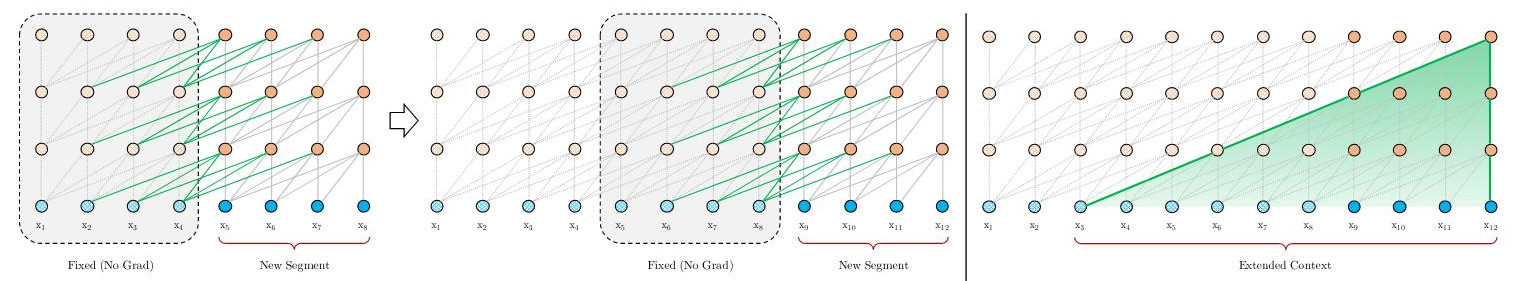
\includegraphics[width=1\textwidth]{xt}
    \caption{ ساختار شبکه Transformer-XL }
    \label{fig:xt}
\end{figure}

با این که گرادیان به هر بخش به صورت مجزا اعمال می‌شود اما این کار سبب می‌شود که مدل اطلاعات را از
گذشته استخراج کند. که باعث بیشتر شدن طول وابستگی‌های بررسی شده می‌شود و همچنین از 
تکه تکه\footnote{\lr{Fragmentation}}
آنالیز کردن
متن جلوگیری می‌کند.

مزیت دیگری که به واسطه اضافه کردن اتصالات به دست می‌آید،
ارزیابی\footnote{\lr{Evaluation}}
سریع‌تر است. نمایشی که توسط قسمت قبلی به دست آمده است می‌تواند دوباره استفاده شود در حالی که
transformer
اصلی این چنین نیست و باید از ابتدا محاسبه شود. بر اساس بررسی‌های صورت گرفته این مدل از مدل اولیه و اصلی
عمل ارزیابی را ۱۸۰۰ بار سریع تر انجام می‌دهد.

ویژگی دیگر این مدل آن است که این ارتباطات می‌توانند علاوه بر قسمت قبلی به قسمت‌های قبل‌تر نیز ایجاد شوند.
در واقه در تئوری می‌توان این ارتباطات را تا جایی که حافظه‌ی واحد پردازنده گرافیکی اجازه می دهد عمق داد
و از همه‌ی آن‌ها به عنوان به عنوان اطلاعات اضافه استفاده نمود. می‌توان تعداد زیادی حالت نهان از گذشته را به عنوان
cache
ذخیره کرد و از آن به عنوان حافظه استفاده نمود.

اگرچه ایده‌ی استفاده شده بسیار جالب است اما سبب از بین رفتن اطلاعات مکانی کلمات می‌شود. برای حل این
مسئله از شبکه
transformer
اصلی الهام گرفته شده تا با استفاده از
رمزنگاری موقعیتی نسبی\footnote{\lr{Relative Positional Encodings}}
روشی ارائه شود. اما برای آن که این روش با ساختار جدید سازگار باشد تنها اطلاعات موقعیتی نسبی در
لایه‌های پنهان ذخیره می‌شوند. در واقع چیزی که شبکه می‌داند فاصله‌ی هر بردار از خودش است نه
موقعیت مکانی قطعی\footnote{\lr{Absolute Position}}
آن.

این مدل علاوه بر اضافه کردن ارتباطات جدید به شبکه‌ی
\lr{transformer}
روشی برای حل وابستگی‌های طولانی‌تر ارائه داد و همچنین ساختاری برای نگهداری موقیت بردارها ایجاد نمود. علاوه بر این‌ها
سرعت این مدل از مدل
\lr{transformer}
اصلی تا حد زیادی بالاتر است. مدل معرفی شده در
مدل سازی زبان\footnote{\lr{Language Modeling}}
عملکرد بسیار خوبی دارد.


\subsection{بررسی چند مقاله}

یکی دیگر از بخش‌های استخراج اطلاعات
شناخت موجودیت\footnote{\lr{Named Entity Recognition}}
است. بیشتر روش‌های موجود از روش‌های دستی برای انتخاب ویژگی و شناسایی استفاده می‌کنند. در مقاله
\cite{lample2016neural}
شبکه‌ای بر پایه
\lr{LSTM}
دوطرفه برای استفاده از شبکه‌های عمیق به جای به دست آوردن ویژگی‌ها به صورت دستی ارائه شده‌است. 

در مقاله‌ی
\cite{ma2016endtoend}
یک مدل
\lr{end-to-end}
برای
لیبل گذاری دنباله\footnote{\lr{Sequence Labeling}}
ارائه شد. این مدل از به هم پیوستن چند شبکه‌ی مختلف که هر کدام ویژگی‌های منحصر به خود را دارند
تشکیل شده‌است. بخش اول که با داده‌ی ورودی سر و کار دارد یک شبکه
\lr{CNN}
است. هدف استفاده از این شبکه دست یابی به نمایش برداری در سطح حروف است. در واقع کلمات ورودی
به این شبکه به نمایش برداری در سطح حرف تبدیل می‌شوند که ورودی شبکه
\lr{LSTM}
را تشکیل می‌دهند.
سپس این نمایش برداری از حروف با نمایش برداری در سطح کلمات ترکیب می شوند و به شبکه
\lr{LSTM}
دو طرفه داده می‌شوند. سپس خروجی شبکه
\lr{BLSTM}
به شبکه
\lr{CRF}
داده می‌شود. در لیبل گذاری دنباله‌ استفاده از همبستگی لیبل‌های همسایه‌ی یکدیگر می‌تواند کمک شایانی در افزایش دقت مدل
کند. به همین دلیل استفاده از
فیلد تصادفی شرطی\footnote{\lr{Conditional Random Field}}
می‌تواند به مدل کمک کند. 

شبکه‌ی
\lr{BERT}
عملکرد خوبی در بسیاری از موارد مربوط به پردازش زبان و گفتار طبیعی دارد. اما استفاده از
ماسک کردن ورودی\footnote{\lr{Input Masking}}
می‌تواند سبب عدم دقت مدل به وابستگی‌های بین نقاط ماسک شده شود. در
\cite{yang2020xlnet}
مدل
\lr{XLNet}
معرفی شده‌است که با استفاده از
یادگیری تعمیم یافته‌ی خود رگرسیون\footnote{\lr{Gneralized Autoregressive}}
سعی در حل این مسئله داشته‌اند.

اسناد ممکن است ترکیب بندی\footnote{\lr{Layout}}
های مختلفی داشته باشند. به عنوان مثال یک سند می‌تواند فقط شامل متن باشد، یا از تصاویر و جداول درون آن استفاده‌
شده باشد. بدون در نظر گرفتن این چیدمان استخراج اطلاعات از جدول‌ها و غیره کار دشواری است. در
\cite{denk2019bertgrid}
با استفاده از
\lr{BERT}
و یک
توری\footnote{\lr{Grid}}
که در سطح کلمه ساخته می‌شود دقت استخراج اطلاعات در اسنادی که تنها متن خالی نیستند را بالا برده‌است. در
\cite{katti2018chargrid}
که یکسال قبل از این مقاله ارائه شده بود نیز از روش توری در سطح حرف و شبکه‌ی کانولوشنال برای
این مسئله استفاده شده بود. توری گذاری در تصویر
\ref{fig:grid}
نمایش داده شده‌است.

\begin{figure}[!ht]
    \centering
    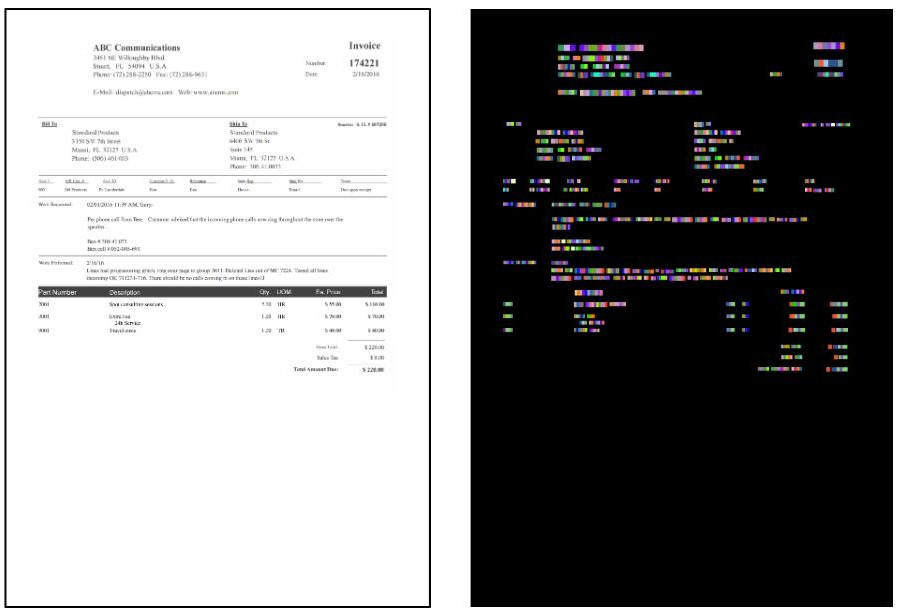
\includegraphics[width=0.6\textwidth]{grid}
    \caption{ سند اصلی در کنار توری شده‌ی آن }
    \label{fig:grid}
\end{figure}

\section{روش‌های بر پایه خلاصه سازی متن}

موفقیت‌های اخیر یادگیری دنباله به دنباله\footnote{\lr{Sequence-to-Sequence Learning (seq2seq)}}
و کسب موفقیت در بسیاری از مسئله‌های پردازش زبان و گفتار طبیعی، نوید موفقیت در این زمینه را می‌دهدد. همچنین
تعدادی مدل بر اساس
RNN
توانسته‌اند دقت‌های خوبی در خلاصه سازی متون کوتاه به دست آورند.
اما این روش‌ها علارقم پیشرفت چشم‌گیری که داشته‌اند هنوزهم در برخی موارد به ویژه دو مورد زیر
دچار مشکلاتی هستند
\cite{el2021automatic}

\begin{enumerate}
    \item تولید کلمات و عبارات تکراری
    \item عدم موفقیت در مواجهه با کلمات خارج از دایره لغات\footnote{\lr{Out-of-Vocabulary (OOV) Words}}
\end{enumerate}

\subsubsection{\lr{ATSDL}}

خلاصه سازی متن انتزاعی\footnote{\lr{Abstractive Text Summarization (ATS)}}
عملی برای ایجاد خلاصه‌ی متن با انتخاب حقایق از جملات متن و در کنار هم قرار دادن آن‌ها برای رسیدن به یک
نمایش کوتاه‌تر است. نکته‌ی مهم آن است که باید معنا و مفهوم کلی متن به خوبی در خلاصه‌ی ایجاد شده حفظ شود.
در مقاله‌ی
\cite{song2019abstractive}
یک مدل بر اساس
\lr{LSTM}
و
\lr{CNN}
ارائه شده‌است که قادر است با جست و جو در بخش‌های بسیار کوچک متن نسبت به جملات عمل خلاصه سازی انتزاعی
متن را انجام دهد.
این شبکه از دو بخش تشکیل شده‌است، بخش اول که عبارات را از متن اصلی استخراج می‌کند
و بخش بعدی که وظیفه‌ی آن ساخت متن نهایی از این عبارات استخراج شده است.
برای بررسی مدل دو دیتاست
\lr{CNN}
و
\lr{DailyMail}
استفاده شده‌است. 

همان‌طور که گفته شده مدل
\lr{Seq2Seq}
یکی از موفق‌ترین مدل‌های ارائه شده در این زمینه است، این مدل نیز از
\lr{Sqe2Seq}
الهام گرفته‌است تا بتواند با استفاده از و بهبود آن نتیجه‌ی بهتری کسب کند.
به مانند
\lr{Sqe2Seq}
این مدل دارای ساختار
رمزنگار-رمزگشا\footnote{\lr{Endoder-Decoder Structure}}
است. در بخش رمزنگار این مدل داده‌ی ورودی را در سطح جمله دریافت می‌کند. با این کار مدل از
عبارات درون جمله برای استخراج معنا استفاده می‌کند. برای بهتر شدن این کار قبل از وارو شدن جملات به
مدل، استخراج عبارات\footnote{\lr{Phrase Extraction}}
صورت می‌گیرد. به آن معنا که مشخص می‌شود هر عبارت چه ساختاری دارد. در واقع عبارات به
دسته‌های عبارات اسمی، فعلی، فاعلی و مفعولی تقسیم می‌شوند. 

در این مدل از شبکه
\lr{CNN}
برای رمزنگاری استفاده شده‌است. دلیل آن هم قابلیت یادگیری تک لایه و همچنین عملکرد خوب و ثابت شده‌ی
این شبکه‌ها در مسئله‌های پردازش زبان و گفتار در سطح جمله است. ورودی به شبکه‌ی
\lr{CNN}
وارد می‌شود. پس از آن یک لایه
\lr{max pooling}
وجود دارد. در این بخش از کرنل‌های با ابعد مختلف استفاده شده‌است تا
بردار‌های عبارات\footnote{\lr{Phrase Vectors}}
مختلفی حاصل شوند.

بخش بعدی شبکه‌ی
\lr{RNN}
است که همان طور که گفته شد وظیفه‌ی آن تولید متن نهایی خلاصه شده است.
در مقاله‌های مختلفی قدرت
LSTM
و
GRU
برای انجام این سبک از مسائل ثابت شده‌است. شبکه‌های
GRU
از نظر محاسباتی سریع‌تر و کم هزینه‌تر هستند اما 
LSTM
ها قدرت بالاتری در بهبود پارامترها دارند و همچنین از لحاظ تئوری از شانس موفقیت بالاتری برخوردار هستند.
در شکل
\ref{fig:ATSDL}
فرایند این مدل از ابتدا تا انتها آورده شده‌است.

\begin{figure}[!ht]
    \centering
    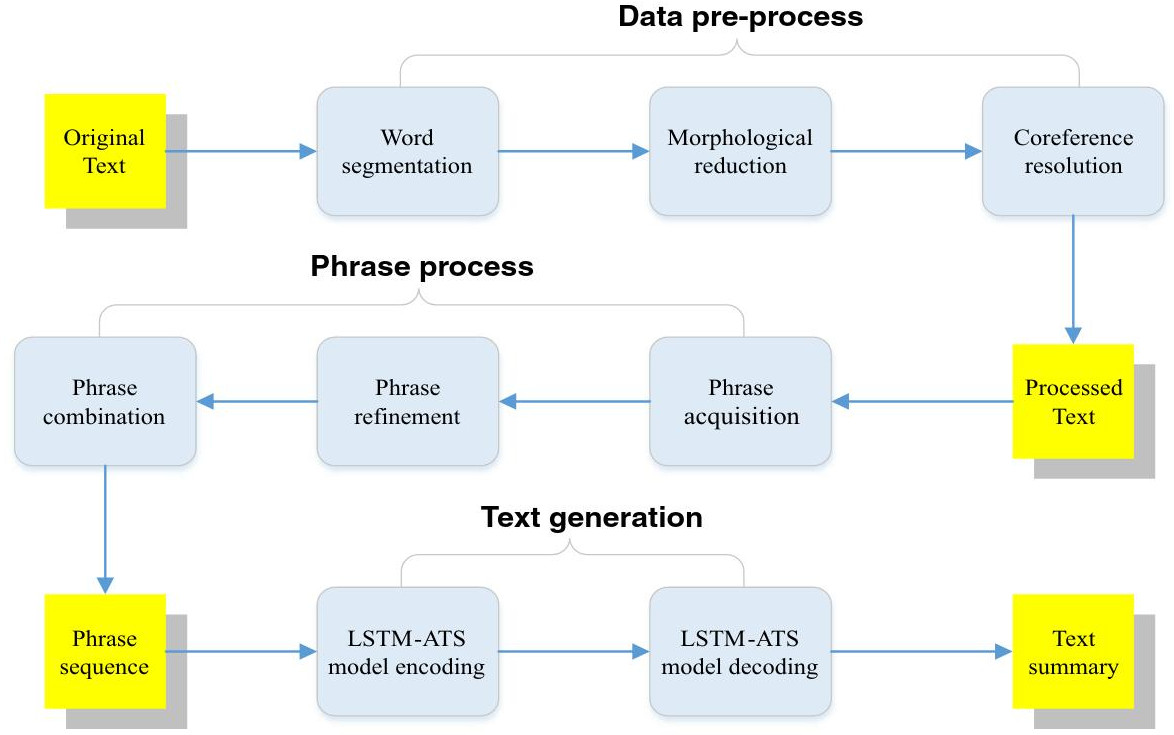
\includegraphics[width=0.7\textwidth]{ATSDL}
    \caption{فرایند مدل ATSDL}
    \label{fig:ATSDL}
\end{figure}

\subsubsection{ویکیپدیا و ترنسفورمر}

یکی از منابع مهم اطلاعات متنی در دنیای وب سایت ویکیپدیا است. در مقاله‌ی 
\cite{liu2018generating}
از ویکیپدیای انگلیسی به عنوان منبعی برای یادگیری مدل برای امر خلاصه سازی متون چند سند استفاده می‌شود.
در این مقاله با استفاده از ترکیب دو روش
\lr{abstractive}
و
\lr{extractive}
مدلی بر پایه‌ی شبکه‌ی
\lr{LSTM}
و
\lr{transformer}
ارائه شده‌است.

به دلیل استفاده از ویکیپدیا به عنوان دیتاست و حجم زیاد آن، نمی‌توان مدل را به صورت
\lr{end-to-end}
یادگیر کرد. پس مدل به دو بخش تقسیم شده است. بخش اول که همان بخش
\lr{extractive}
مدل است، وظیفه دارد تا اطلاعات را از متون استخراج کند. الگوریتم ارائه شده به این شکل است که به پاراگراف‌های
متن یک لیست درست می‌شود که شامل رتبه\footnote{\lr{Rank}}
آن پاراگراف نیز هست. برای این کار
\lr{L}
توکن اول هر پاراگراف گرفته می‌شود. ۴ نوع رنک دهی استفاده می‌شود.

\begin{enumerate}
    \item فرض می‌شود که می‌خواهیم عمل بازیابی با عبارت را انجام دهیم\footnote{\lr{Query Retrieval}}
          و عبارت جست و جو شده عنوان سند است. برای این کار
          \lr{tf-idf}
          محاسبه می‌شود.
    \item الگوریتم
          \lr{TextRank}
          استفاده می‌شود. یک گراف تشکیل می‌دهد که واحدهای متنی گره‌ها هستند و یال‌ها بر اساس
          همپوشانی کلمات تشکیل می‌شوند. سپس از الگوریتمی شبیه به
          \lr{PageRank}
          برای نمره دهی استفاده می‌شود.
    \item الگوریتم
          \lr{SumBasic}.
          در این روش تعداد کلمات محاسبه می‌شود، و از این تعداد برای نمره دهی به کلمات استفاده می‌شود.
          سپس از امتایازات کلمات امتیاز جمله‌ها به دست می‌آید. پس از این کار بهترین جمله انتخای می‌شود و
          امتیاز کلمات آن کاهش می‌یابد. این کار تکرار می‌شود تا به یک جمع مورد نظر برسیم.
    \item برای نمایش اهمیت استخراج‌ از یک روش دیگر که به عنوان تقلب از آن یاد می‌شوند
          استفاده می‌کنند. در این روش از
          \lr{bigram}
          برای به دست آوردن اهمیت استفاده می‌شود.
\end{enumerate}

پس از استخراج پاراگراف‌های مهم متنی با به هم چسباندن این پاراگراف‌ها به ترتیب اهمیتشان ایجاد می‌شود.
سپس کلمات با استفاده از روش
\lr{Sub-word Tokenization}
رمزنگاری می‌شوند. سپس از یک رمزگشای بر پایه
transformer
برای تولید متن استفاده می‌شود.


\subsection{بررسی چند مقاله}

در
\cite{zhang2018extractive}
از روش
خلاصه سازی سند استخراجی\footnote{\lr{Extractive Document Summarization}}
برای این کار استفاده ‌شده‌است. مدل معرفی شده از شبکه‌ی
\lr{GRU}
سلسله مراتبی استفاده می‌کند که از دو مرحله تشکیل شده‌است.

\begin{enumerate}
    \item استخراج جمله‌ی کلیدی با استفاده از فرمول فاصله لونشتاین\footnote{\lr{Levenshtein Distance Formula}}
    \item استفاده از شبکه‌ی عصبی برای امر خلاصه سازی
\end{enumerate}

در مرحله‌ی استخراج سیستم ترکیبی از نمایش برداری جملات و فاصله‌ی لونشتاین را به عنوانی معیاری
هیبرید استفاده می‌کند تا از آن جملات کلیدی را استخراج کند.
مرحله‌ی بعدی تولید متن نهایی است. در این مرحله کل سند و همچنین جملات مهم به یک شبکه
\lr{GRU}
داده می‌شود و این شبکه با استفاده از ویژگی‌های موجود به تولید متن خلاصه شده می‌پردازد.

برخی از مقالات به خلاصه سازی چندین متن پرداخته اند. این نوع خلاصه سازی
با استفاده از شبکه های عمیق از سال ۲۰۱۵ شروع شد. مقاله‌ی
\cite{li2017cascaded}
همین کار را انجام می‌دهد. در این مقاله یک مدل بر اساس شبکه‌های
\lr{RNN}
ارائه شد. هدف این مدل بررسی اطلاعات برجسته در اسناد از روش نظارت نشده است. 
در این روش اطلاعات برجسته از جملات تشکیل نمایش برداری را می‌دهند.
در این روش از مکانیزم توجه برای تمرکز بر بازسازی جملات استفاده شده‌است.
در واقع مدل پیشنهادی ترکیبی از
\lr{LSTM}
و
مکانیزم ‌توجه است.

در
\cite{amplayo2021informative}
بیان شد که خلاصه‌هایی که در مدل‌های مختلف تولید می‌شوند، از دقت و اطلاعات کافی برخوردار نیستند و نمی‌توانند
بر اساس ترجیحات خلاصه‌های مد نظر را تولید کنند. برای رفع این نواقص در این مقاله مدلی دو بخشی ارائه کردند و
به عمل خلاصه سازی به عنوان کاری برای انتقال چند وجهی اطلاعات نگاه کردند تا بتوانند اطلاعات برجسته
را از اسناد دریافت کنند و انتقال دهند.

برای هر سند ورودی از یک شبکه
\lr{LSTM}
دو طرفه رمزنگار استفاده کردند تا نمایش برداری در سطح سند و در سطح کلمه را یادگیری کند.
اطلاعات حالت‌های پنهان در هر دو جهت شبکه با یکدیگر تشکیل نمایش برداری سطح کلمه را می دهند.
نمایش برداری سطح سند نیز تشکیل شده از مجموع نمایش برداری کلمه‌ی اول و کلمه‌ی آخر سند است.
در آخر از یک شبکه
\lr{LSTM}
به همراه مکانیزم توجه برای رمزگشایی استفاده شده‌است.

یکی از راه‌هایی که می‌توان از شیکه‌های
\lr{CNN}
برای خلاصه سازی اسناد چندتایی\footnote{\lr{Multi Document Summarization}}
استفاده کرد آن است که تعدادی کرنل با ابعا مختلف را روی اسناد ورودی حرکت داد تا به نمایشی معنایی از
اسناد رسید. در
\cite{ziqiang2015prior}
یک مدل بر پایه
\lr{CNN}
ارائه شد که از روش گفته شده استفاده می‌کند. در این مقاله اسناد به شبکه‌ی کانولوشنال داده می‌شوند و سپس
از دو لایه
\lr{max-over-time pooling}
گذر می‌کنند. این روش در مقایسه با استفاده از شبکه کانولوشنال ساده از عملکرد بهتری برخوردار است. دلیل آن هم
استخراج اطلاعات مستقل از سند برای امر خلاصه سازی است.

در
\cite{liu2019hierarchical}
یک مدل مبتنی بر
transformer
ارائه شد که از دو مکانیزم توجه بین پاراگرافی\footnote{\lr{Inter-paragraph}}
و همچنین
\lr{graph-informed}
استفاده می‌کند. این کار به مدل اجازه می‌دهد تا چند متن را به جای به هم پیوستن
به صورت سلسله مراتبی مورد بررسی قرار دهد. در این مدل برای رمزگشا از یک
transformer
ابا ساختار اصلی استفاده شده و همچنین برای خلاصه‌هایی با طول بسیار کم و با عدم داشتن اطلاعات کافی از متن
مجازات در نظر گرفته شده‌است. علاوه بر این یک شبکه رگرسیون منطقی\footnote{\lr{Logistic Regression Model}}
نیز برای انتخاب پاراگراف‌های برتر اضافه شده‌است.

\section{روش‌های بر پایه خوشه بندی}

\subsubsection{\lr{STCC}}

خوشه بندی متون کوتاه به دلیل پراکندگی و گستردگی نمایش متن عملی چالش برانگیز است.
در
\cite{Xu2017}
یک شبکه کلنولوشنال خودآموز\footnote{\lr{Self-Taught}}
برای این کار معرفی شده‌است که می‌تواند اطلاعات معنایی بیشتر و کاربردی‌تری  را دریافت و پردازش کند.
در این مدل در ابتدا متن خام با استفاده از یکی از روش‌های کاهش بعد بدون نظارت\footnote{\lr{Unsupervised Dimensionality Reduction}}
به نمایش دودویی\footnote{\lr{Binary}}
تبدیل می‌شود سپس به شبکه‌ی کانولوشنال داده می‌شوند تا ویژگی‌های پیچیده‌ی آن‌ها یادگیری شوند.
سپس با استفاده از یک خوشه بند
\lr{K-means}
نمایش خوشه‌ای متون یادگیری می‌شود.

نمایش
\lr{BOW}
متن برای این که به شبکه‌ی
\lr{CNN}
داده شود با استفاده از یکی از روش‌های کاهش بعد به نمایش دودیی تبدیل شود. این کار دربافت بهتر اطلاعات
در بخش کانولوشنی مدل می‌شود و به نوعی این بخش را هدایت می‌کند. در نهایت هر متن ورودی به نمایش
ماتریسی تبدیل می‌شود.

\begin{figure}[!ht]
    \centering
    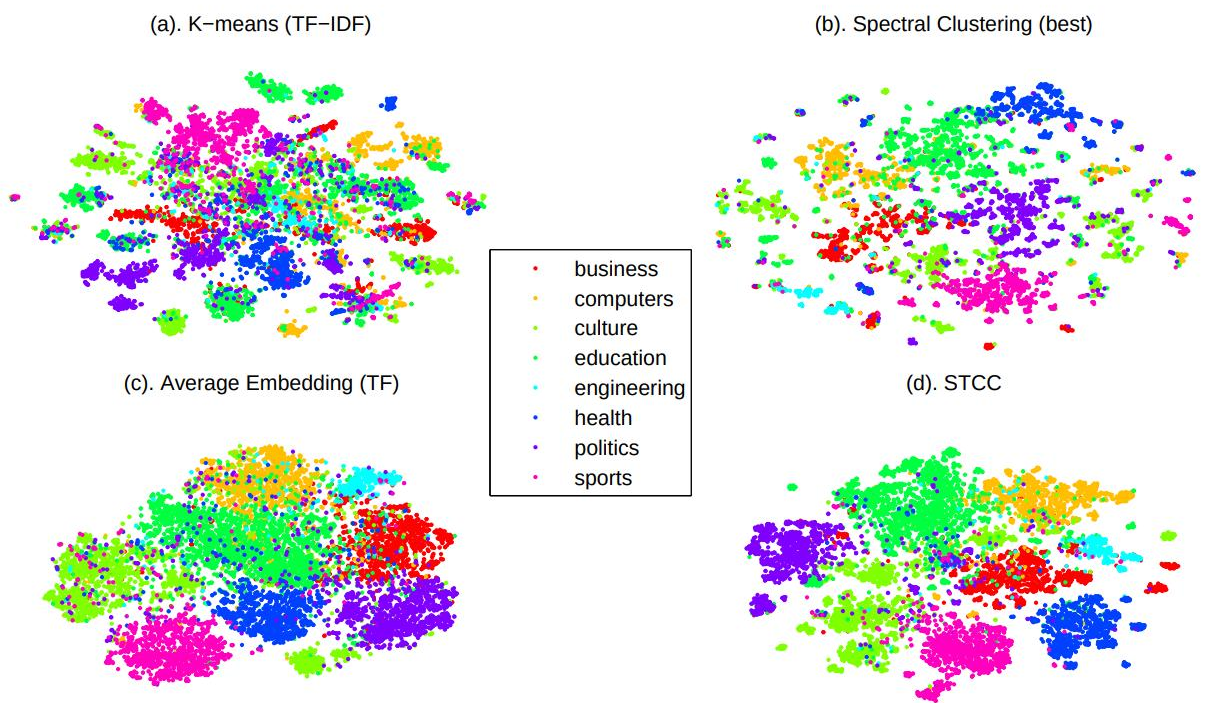
\includegraphics[width=0.8\textwidth]{STCC}
    \caption{عملکرد مدل STCC}
    \label{fig:STCC}
\end{figure}

بخش کانولوشنال از یک لایه کانولوشنال عریض و بعد از آن یک لایه
\lr{k-max pooling}
استفاده شده‌است. سپس از یک لایه‌ی کانولوشنی عریض\footnote{\lr{Wide Convolution}}
به همراه
\lr{folding}
که کار آن جمع هر دو سطر بردار ویژگی‌ها است  استفاده شده‌است. لایه‌ی آخر نیز مجدد یک لایه 
\lr{k-max pooling}
می‌باشد. در آخر نیز با استفاده از خروجی شبکه، الگوریتم خوشه بندی
\lr{K-means}
اجرا می‌شود. در شکل
\ref{fig:STCC}
عملکرد این مدل آمده‌است.

\subsection{بررسی چند مقاله}
در
\cite{zhou2019endtoend}
مدلی برای خوشه بندی متون به صورت
\lr{end-to-end}
ارائه شد. معمولا اکثز مدل‌ها برای رسیدن به خوشه بندی‌های مناسب این عمل را به چند بخش تقسیم می‌کنند.
یادگیری نمایش متن\footnote{\lr{Text Representation Learning}}
و خوشه بندی نمایش یادگیری شده دو بخش اصلی اکثر این مدل‌ها هستند. برخی نیز برای حل مشکل
پراکندی و گستردگی از مدل‌های بر پایه شبکه‌های عصبی در بخش یادگیری نمایش متن استفاده کردند.
اما بار هم یک فرایند چند مرحله‌ای انجام می‌شود. که مرحله‌ی بعدی آن عموما
\lr{K-means}
است.

در این مقاله روشی بر پایه شبکه‌های عصبی برای یادگیری تماما
\lr{end-to-end}
ارائه شده‌است که توامان نمایش متن و خوشه بندی را یادگیری می‌کند. این مدل بر روی دو دیتاست معروف
\lr{IMDB}
و
\lr{20-Newsgroup}
آزمایش شده‌است.

بیشتر الگوریتم‌های خوشه بندی سعی در حل مسئله به صورت پیمایشی دارند. و هدف آن‌ها این است که بفهمند
داده‌ی کنونی به کدام خوشه تعلق دارد. اما در این مدل به این سوال که آیا دو نمونه‌ی انتخاب شده به یک
خوشه‌ی یکسان تعلق دارند پاسخ داده می‌شود.

در این مدل از
\lr{LSTM}
دو طرفه برای پردازش داده‌ی ورودی استفاده شده‌است. از این شبکه نمایش متن به دست می‌اید. سپس از یک عملگر
ماکزیمم استفاده می‌شود. لایه‌ی بعدی یک سافت‌مکس است تا با استفاده از آن از نمایش به دست آمده
به یک نمایش برداری برسیم.

\begin{figure}[!ht]
    \centering
    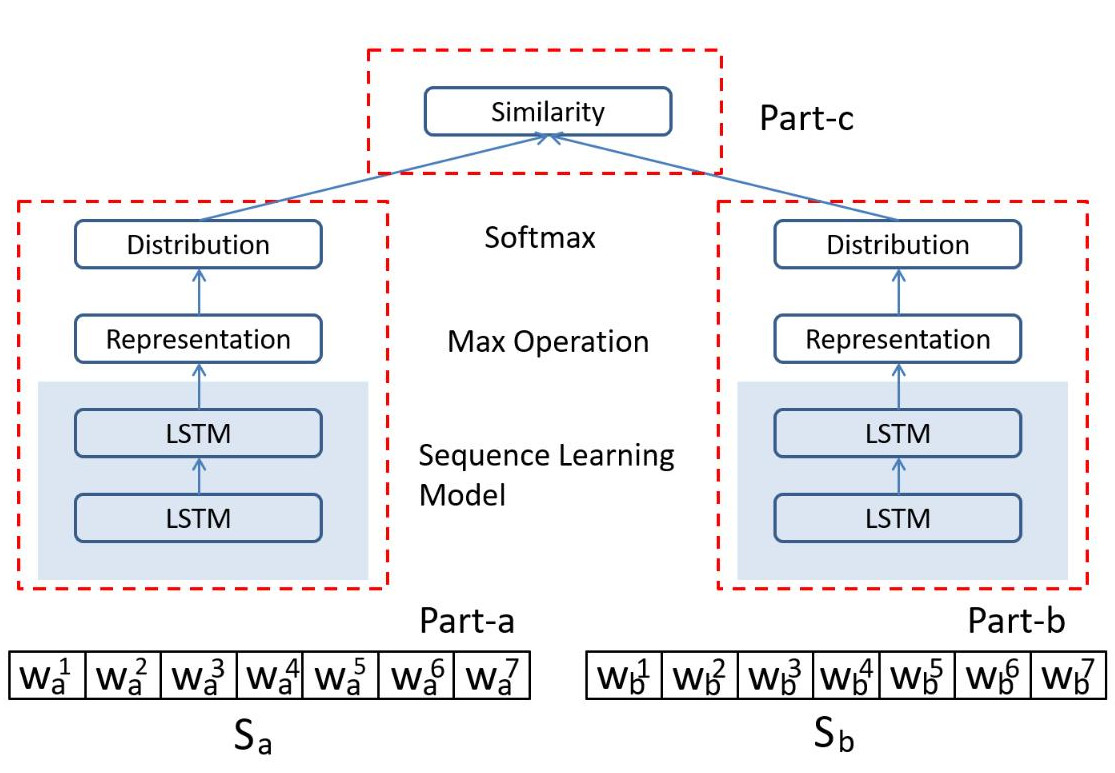
\includegraphics[width=0.7\textwidth]{e2e}
    \caption{ساختار مدل خوشه بند \lr{end-to-end}}
    \label{fig:e2e}
\end{figure}

سپس از نمایش‌های برداری به دست آمده استفاده می‌شود تا تخمین زد که آیا دو جمله‌ی هب دست آمده به یک
خوشه تعلق دارند یا خیر. ساغختار مدل در شکل
\ref{fig:e2e}
آمده است.

خوشه بندی یکی از عملیات‌های مهم متن کاوی است، این عمل به شکل گسترده در
بازیابی اطلاعات\footnote{\lr{Information Retrieval}}
و
ادغام متن\footnote{\lr{Text Integration}}
استفاده می‌شود. در مدل‌های جدید و با استفاده از یادگیری عمیق شبکه‌هایی به صورت ترکیبی ارائه می‌شوند که
یادگیری نمایش و استخراج اطلاعات در آن‌ها بر عهده‌ی شبکه‌های عمیق است و معمولا با استفاده از 
الگوریتم‌های خوشه بندی کلاسیک اقدام به شناخت خوشه‌ها می‌کنند.
\cite{fan2018neural}
با استفاده از مدلی شامل
شبکه‌های‌
\lr{LSTM}
و
\lr{CNN}
و همچنین الگوریتم خوشه بندی
\lr{K-means}
به انجام عمل خوشه بندی متون با استفاده از شبکه‌های عمیق می‌پردازد. در این مدل اطلاعات به دست امده
از خوشه بندی به عنوان
\lr{feed-back}
به مدل داده می‌شوند که سبب می‌شود مدل در طول زمان خود را بهبود بخشد.

در این مدل متن خام وارد بخش پیش پردازش می‌شود، در این بخش عملیات توکتن سازی انجام می‌شود و همچنین
\lr{stop words}
حذف می‌شوند. سپس به لایه‌ی
\lr{LSTM}
دو طرفه می‌رسیم. هدف این بخش استخراج اطلاعات معنایی از متون توکن شده است. شبکه‌ی
\lr{LSTM}
دو طرفه کاربرد زیادی در مسئله‌های مربوط به متون دارند، در این روش نیز با توجه به کار‌های گذشته از یک
شبکه‌ی دو طرفه برای به دست آوردن اطلاعات و استخراج آن‌ها استفاده شده‌است.

شبکه‌ی
\lr{CNN}
برای دست‌یابی به اطلاعات نهان در متن اصلی استفاده می‌شود. همان طور که گفته شد شبکه‌های کانولوشنال
با توجه به ساختاری که دارند قابلیت درک بالایی در استخراج اطلاعات و وابستگی‌های محلی دارند. اطلاعات به دست آمده
توسط لایه قبلی در این لایه پردازش می‌شوند تا با استفاده از این شبکه اطلاعات عمیق‌تری استخراج شوند.
هنگام کار با
\lr{CNN}
ها نکته‌ای که بسیار اهمیت دارد آن است که اندازه و ابعاد کرنل‌ها چه مقداری باشند. اگر کوچک باشند ممکتن است
سبب از بین رفتن بسیاری از اطلاعات مهم شوند، در مقابل بزرگ بودن ابعاد سبب بالا رفتن تعداد پارامتر‌ها می‌شود که این
مسئله خود مشکلاتی مثل پیچیدگی مدل،
\lr{overtrain}
شدن مدل و همچنین مشکل شدن فرایند یادگیری را حاصل می‌شود.

در مرحله‌ی آخر نیز از الگوریتم
\lr{K-means}
استفاده می‌شود تا عملیات خوشه بندی انجام شود. از این خوشه‌های به دست آمده استفاده می‌شود تا مدل را بهینه سازی کرد.
در واقع
\lr{feed-back}
هایی وجود دارند که مدل با استفاده از ان‌ها خود را بهبود می‌بخشد.

\chapter{جمع‌بندی و نتیجه‌گیری}
\pagebreak
\section{مقدمه}

در این بخش با توجه به مسائل و مدل‌های یررسی شده در فصل قبل به جمع بندی و همچنین ارائه پیشنهاداتی برای
امکان بهتر شدن مدل‌ها پرداخته می‌شود. همان طور که در فصل پیش مشاهده شد، متن کاوی رویکردهای مختلفی را
شامل می‌شود و هر کدام از این رویکرد‌ها روش‌های متعددی دارند. از میان این روش‌ها تعدادی از روش‌های مبتنی
بر یادگیری عمیق بررسی شدند که به ما دید مناسبی برای بررسی و ارائه نظر می‌دهد.

\section{جمع بندی و ارائه پیشنهاد}

در اکثر روش‌هایی که معرفی شد از شبکه‌های
\lr{RNN}
یا به طور مستقیم یا در بخشی از مدل استفاده شد. همان طور که جدول
\ref{fig:dist}
نشان می‌دهد، روش‌های مبتنی بر
\lr{RNN}
به خصوص
\lr{LSTM}
جایگاه ویزه‌ای در پردازش زبان و گفتار طبیعی و متن کاوی دارند.

\begin{figure}[!ht]
    \centering
    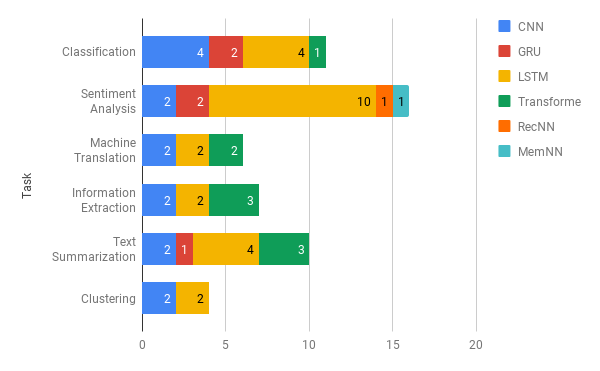
\includegraphics[width=\textwidth]{dist}
    \caption{پراکندگی شبکه‌های استفاده شده}
    \label{fig:dist}
\end{figure}

به راحتی می‌توان به این موضوع دست یافت که شبکه‌های
\lr{LSTM}
عملکرد خوبی در این زمینه دارند و این مسئله سبب استفاده‌ی پر تکرار از آن‌ها شده‌است.

با توجه به مقاله‌های بررسی شده می‌توان دریافت که شبکه‌های
\lr{RNN}
دو طرفه بهتر قادرند تا نمایشی از متن ورودی به دست آوند. همچنین بنا بر میزان اهمیت وابستگی‌های متن
می‌توان یکی از سه مدل
\lr{CNN}
،
\lr{LSTM}
و یا
\lr{Transformer}
را انتخاب کرد که به ترتیب از وابستگی‌‌های کوتاه تا بلند را بررسی می‌کنند.

در صورتی که بخش‌های ورودی همه از اهمیت یکسانی برخوردار نیستند، مکانیزم توجه به خوبی خود را نشان می‌دهد.
به عنوان مثال در امر خلاصه سازی متن که می‌خواهیم قسمت‌های مهم متن را انتخاب کنیم، استفاده از مکانیزم توجه
سبب تمرکز بهتر مدل می شود. همچنین در صورتی که بردار ورودی ترکیبی از نمایش‌های مختلف به عنوان مثال
ترکیب نمایش در سطح کلمه و حرف باشد استفاده از مکانیزم توجه موثر است.

شبکه‌های
\lr{CNN}
وابستگی‌های محلی را به خوبی به دست می‌اوردن اما مسئله‌ی مهم هنگام استفاده از ان‌ها انتخاب دقیق اندازه و سایز کرنل‌
می‌باشد. باید دقت شود که در صورت کوچک بودن آن اطلاعات از دست می‌رود و در صورت بزرگ بودن
مدل بسیار بزرگ می‌شود و یادگیری آن کاری دشوار خواهد بود.

هر چه در سال‌ها رو به جلو می‌رویم استفاده از
\lr{Transformer} 
ها محبوبیت پیدا می‌کند. این مدل‌ها که بر پایه‌ی مکانیزم توجه و یادگیری انتقالی بنا شده‌اند، قدرت خوبی در پردازش متن از
خود نشان داده‌اند. به خصوص مدل
\lr{BERT}
و دیگر مدل‌های بر پایه و با الهام از آن.

ساختار سلسله مراتبی مدل‌ها با توجه به این که ساختار متون نیز چنین است در برخی مدل‌ها کمک شایانی به
بالا رفتن دقت کرده‌است. می‌توان از این ساختار بهره گرفت و با اسفتاده از آن مدل‌های بهتر و با دقت بیشتری تولید کرد.

برای بهبود فرایندهای مربوط به متن کاوی پییشنهاد می‌شود استفاده از روش‌های بر پایه مکانیزم توجه افزایش یابد،
همچنین استفاده از شبکه‌های دو طرفه می‌تواند به دقت مدل کمک کند. در مسائل پیچیده تر
\lr{ensemble learning}
می‌تواند بسیار موثر باشد. ترکیب سه مدل برتر گفته شده ممکن است سبب بالاتر رفتن دقت مدل‌ها شود.
در ادامه نیز جدولی از مدل‌های بررسی شده آمده است که بسیاری از نتیجه گیری‌های انجام شده بر اساس آن می‌باشد.

\pagebreak

\begin{tiny}
\begin{latin}
    \begin{longtable}{|c|c|c|c|c|c|cc|}
        \hline
        Paper & Year & Network(s) & Attention & Information & Dataset(s) & Metric(s) & Score \\ \hline
        \multicolumn{8}{|c|}{Classificaion}                                                                                                                                                                                                                                                                                                                                                                                                                                        \\ \hline
        \multirow{2}{*}{\cite{johnson-zhang-2015-effective}} & \multirow{2}{*}{2015} & \multirow{2}{*}{CNN}              & \multirow{2}{*}{-}                      & \multirow{2}{*}{BOW}                                                                                   & \multirow{2}{*}{RCV1}                 & \multicolumn{1}{c|}{Micro-F}                                                                                                       & 84.0   \\ \cline{7-8} 
                                                                              &                       &                                   &                                         &                                                                                                        &                                       & \multicolumn{1}{c|}{Macro-F}                                                                                                       & 64.8   \\ \hline
        \multirow{6}{*}{\cite{yang-etal-2016-hierarchical}}  & \multirow{6}{*}{2016} & \multirow{6}{*}{GRU}              & \multirow{6}{*}{Hierarchical Attention} & \multirow{6}{*}{-}                                                                                     & Yelp 2013                             & \multicolumn{1}{c|}{\multirow{6}{*}{Accuracy}}                                                                                     & 68.2   \\ \cline{6-6} \cline{8-8} 
                                                                              &                       &                                   &                                         &                                                                                                        & Yelp 2014                             & \multicolumn{1}{c|}{}                                                                                                              & 70.5   \\ \cline{6-6} \cline{8-8} 
                                                                              &                       &                                   &                                         &                                                                                                        & Yelp 2015                             & \multicolumn{1}{c|}{}                                                                                                              & 71.0   \\ \cline{6-6} \cline{8-8} 
                                                                              &                       &                                   &                                         &                                                                                                        & IMDB                                  & \multicolumn{1}{c|}{}                                                                                                              & 49.4   \\ \cline{6-6} \cline{8-8} 
                                                                              &                       &                                   &                                         &                                                                                                        & Yahoo Answer                          & \multicolumn{1}{c|}{}                                                                                                              & 75.8   \\ \cline{6-6} \cline{8-8} 
                                                                              &                       &                                   &                                         &                                                                                                        & Amazon                                & \multicolumn{1}{c|}{}                                                                                                              & 63.6   \\ \hline
        \multirow{6}{*}{\cite{conneau2016very}}              & \multirow{6}{*}{2016} & \multirow{6}{*}{CNN}              & \multirow{6}{*}{-}                      & \multirow{6}{*}{Residual Connections}                                                                  & AG’s news                             & \multicolumn{1}{c|}{\multirow{6}{*}{Error}}                                                                                        & 8.73   \\ \cline{6-6} \cline{8-8} 
                                                                              &                       &                                   &                                         &                                                                                                        & Sogou news                            & \multicolumn{1}{c|}{}                                                                                                              & 3.36   \\ \cline{6-6} \cline{8-8} 
                                                                              &                       &                                   &                                         &                                                                                                        & DBPedia                               & \multicolumn{1}{c|}{}                                                                                                              & 1.29   \\ \cline{6-6} \cline{8-8} 
                                                                              &                       &                                   &                                         &                                                                                                        & Yelp                                  & \multicolumn{1}{c|}{}                                                                                                              & 35.74  \\ \cline{6-6} \cline{8-8} 
                                                                              &                       &                                   &                                         &                                                                                                        & Yahoo Answers                         & \multicolumn{1}{c|}{}                                                                                                              & 26.57  \\ \cline{6-6} \cline{8-8} 
                                                                              &                       &                                   &                                         &                                                                                                        & Amazon Review                         & \multicolumn{1}{c|}{}                                                                                                              & 37.00  \\ \hline
        \cite{graves2005framewise}                           & 2005                  & Bi-LSTM                           & -                                       & -                                                                                                      & TIMIT                                 & \multicolumn{1}{c|}{Accuracy}                                                                                                      & 70.2   \\ \hline
        \multirow{4}{*}{\cite{liu2016recurrent}}             & \multirow{4}{*}{2016} & \multirow{4}{*}{LSTM}             & \multirow{4}{*}{-}                      & \multirow{4}{*}{-}                                                                                     & SST-1                                 & \multicolumn{1}{c|}{\multirow{4}{*}{Accuracy}}                                                                                     & 49.6   \\ \cline{6-6} \cline{8-8} 
                                                                              &                       &                                   &                                         &                                                                                                        & SST-2                                 & \multicolumn{1}{c|}{}                                                                                                              & 87.9   \\ \cline{6-6} \cline{8-8} 
                                                                              &                       &                                   &                                         &                                                                                                        & SUBJ                                  & \multicolumn{1}{c|}{}                                                                                                              & 94.1   \\ \cline{6-6} \cline{8-8} 
                                                                              &                       &                                   &                                         &                                                                                                        & IMDB                                  & \multicolumn{1}{c|}{}                                                                                                              & 91.3   \\ \hline
        \cite{dieng2016topicrnn}                             & 2016                  & GRU                               & -                                       & Local Dependecies                                                                                      & IMDB                                  & \multicolumn{1}{c|}{Error}                                                                                                         & 6.28   \\ \hline
        \multirow{5}{*}{\cite{miyato2017adversarial}}        & \multirow{5}{*}{2017} & \multirow{5}{*}{LSTM}             & \multirow{5}{*}{-}                      & \multirow{5}{*}{Adversarial training}                                                                  & IMDB                                  & \multicolumn{1}{c|}{\multirow{5}{*}{Error}}                                                                                        & 5.91   \\ \cline{6-6} \cline{8-8} 
                                                                              &                       &                                   &                                         &                                                                                                        & Elec                                  & \multicolumn{1}{c|}{}                                                                                                              & 5.40   \\ \cline{6-6} \cline{8-8} 
                                                                              &                       &                                   &                                         &                                                                                                        & RCV1                                  & \multicolumn{1}{c|}{}                                                                                                              & 6.68   \\ \cline{6-6} \cline{8-8} 
                                                                              &                       &                                   &                                         &                                                                                                        & Rotten Tomatoes                       & \multicolumn{1}{c|}{}                                                                                                              & 16.6   \\ \cline{6-6} \cline{8-8} 
                                                                              &                       &                                   &                                         &                                                                                                        & DBpedia                               & \multicolumn{1}{c|}{}                                                                                                              & 0.76   \\ \hline
        \cite{guggilla-etal-2016-cnn}                        & 2016                  & LSTM-CNN                          & -                                       & Word2Vec                                                                                               & factual vs. feeling                   & \multicolumn{1}{c|}{F1}                                                                                                            & 79.56  \\ \hline
        \multirow{3}{*}{\cite{wang-etal-2016-combination}}   & \multirow{3}{*}{2016} & \multirow{3}{*}{LSTM-CNN}         & \multirow{3}{*}{-}                      & \multirow{3}{*}{\begin{tabular}[c]{@{}c@{}}Word2Vec\\ \\ Short Texts\end{tabular}}                     & MR                                    & \multicolumn{1}{c|}{\multirow{3}{*}{Accuracy}}                                                                                     & 81.52  \\ \cline{6-6} \cline{8-8} 
                                                                              &                       &                                   &                                         &                                                                                                        & SST-1                                 & \multicolumn{1}{c|}{}                                                                                                              & 51.50  \\ \cline{6-6} \cline{8-8} 
                                                                              &                       &                                   &                                         &                                                                                                        & SST-2                                 & \multicolumn{1}{c|}{}                                                                                                              & 89.56  \\ \hline
        \multirow{3}{*}{\cite{johnson-zhang-2017-deep}}      & \multirow{3}{*}{2017} & \multirow{3}{*}{CNN}              & \multirow{3}{*}{-}                      & \multirow{3}{*}{Pyramid Network}                                                                       & Yelp                                  & \multicolumn{1}{c|}{\multirow{3}{*}{Error}}                                                                                        & 30.58  \\ \cline{6-6} \cline{8-8} 
                                                                              &                       &                                   &                                         &                                                                                                        & Yahoo News                            & \multicolumn{1}{c|}{}                                                                                                              & 23.90  \\ \cline{6-6} \cline{8-8} 
                                                                              &                       &                                   &                                         &                                                                                                        & Amazon                                & \multicolumn{1}{c|}{}                                                                                                              & 34.81  \\ \hline
        \cite{schmidt2020data}                               & 2020                  & Transformer                       & Self-attention                          & BERT                                                                                                   & PubMed                                & \multicolumn{1}{c|}{F1}                                                                                                            & 90.0   \\ \hline
        \multicolumn{8}{|c|}{Sentiment Analysis}                                                                                                                                                                                                                                                                                                                                                                                                                                \\ \hline
        \multirow{2}{*}{\cite{68dong-etal-2014-adaptive}}    & \multirow{2}{*}{2014} & \multirow{2}{*}{RecNN}            & \multirow{2}{*}{-}                      & \multirow{2}{*}{Aspect Base}                                                                           & \multirow{2}{*}{Twitter}              & \multicolumn{1}{c|}{Accuracy}                                                                                                      & 66.3   \\ \cline{7-8} 
                                                                              &                       &                                   &                                         &                                                                                                        &                                       & \multicolumn{1}{c|}{Macro-F1}                                                                                                      & 65.9   \\ \hline
        \multirow{2}{*}{\cite{70tang-etal-2016-effective}}   & \multirow{2}{*}{2016} & \multirow{2}{*}{LSTM}             & \multirow{2}{*}{-}                      & \multirow{2}{*}{Aspect Base}                                                                           & \multirow{2}{*}{Twitter}              & \multicolumn{1}{c|}{Accuracy}                                                                                                      & 71.5   \\ \cline{7-8} 
                                                                              &                       &                                   &                                         & Macro-F1                                                                                               &                                       & \multicolumn{2}{c|}{69.5}                                                                                                                   \\ \hline
        \cite{71ruder-etal-2016-hierarchical}                & 2016                  & Bi-LSTM                           & -                                       & \begin{tabular}[c]{@{}c@{}}Aspect Base\\ \\ Hierarchical\end{tabular}                                  & SemEval-2016                          & \multicolumn{1}{c|}{Accuracy}                                                                                                      & 84.8   \\ \hline
        \multirow{2}{*}{\cite{72Zhang_Zhang_Vo_2016}}     & \multirow{2}{*}{2016} & \multirow{2}{*}{Bi-GRU}           & \multirow{2}{*}{-}                      & \multirow{2}{*}{Aspect Base}                                                                           & \multirow{2}{*}{MPQA}                 & \multicolumn{1}{c|}{Accuracy}                                                                                                      & 71.96  \\ \cline{7-8} 
                                                                              &                       &                                   &                                         &                                                                                                        &                                       & \multicolumn{1}{c|}{F1}                                                                                                            & 69.55  \\ \hline
        \multirow{2}{*}{\cite{74YANGATT}}                    & \multirow{2}{*}{2017} & \multirow{2}{*}{LSTM}             & \multirow{2}{*}{Attention Base}         & \multirow{2}{*}{Aspect Base}                                                                           & \multirow{2}{*}{Twitter conversation} & \multicolumn{1}{c|}{Accuracy}                                                                                                      & 72.6   \\ \cline{7-8} 
                                                                              &                       &                                   &                                         &                                                                                                        &                                       & \multicolumn{1}{c|}{F1}                                                                                                            & 72.2   \\ \hline
        \cite{79ma2017interactive}                           & 2017                  & LSTM                              & Attention Base                          & Aspect Base                                                                                            & SemEval 2014                          & \multicolumn{1}{c|}{Accuracy}                                                                                                      & 74.1   \\ \hline
        \cite{73wang-etal-2016-attention}                    & 2016                  & LSTM                              & Attention Base                          & Aspect Base                                                                                            & SemEval 2014                          & \multicolumn{1}{c|}{Accuracy}                                                                                                      & 70.2   \\ \hline
        \cite{76tang2016aspect}                              & 2016                  & MemmNN                            & Attention Base                          & Aspect Base                                                                                            & SemEval 2014                          & \multicolumn{1}{c|}{Accuracy}                                                                                                      & 76.58  \\ \hline
        \multirow{2}{*}{\cite{dos2014deep}}                  & \multirow{2}{*}{2014} & \multirow{2}{*}{CNN}              & \multirow{2}{*}{-}                      & \multirow{2}{*}{Short Texts}                                                                           & SSTb                                  & \multicolumn{1}{c|}{\multirow{2}{*}{Accuracy}}                                                                                     & 48.3   \\ \cline{6-6} \cline{8-8} 
                                                                              &                       &                                   &                                         &                                                                                                        & STS                                   & \multicolumn{1}{c|}{}                                                                                                              & 86.4   \\ \hline
        \multirow{6}{*}{\cite{xu2016cached}}                 & \multirow{6}{*}{2016} & \multirow{6}{*}{Bi-LSTM}          & \multirow{6}{*}{-}                      & \multirow{6}{*}{Caching}                                                                               & \multirow{2}{*}{IMDB}                 & \multicolumn{1}{c|}{Accuracy}                                                                                                      & 46.2   \\ \cline{7-8} 
                                                                              &                       &                                   &                                         &                                                                                                        &                                       & \multicolumn{1}{c|}{MSE}                                                                                                           & 2.112  \\ \cline{6-8} 
                                                                              &                       &                                   &                                         &                                                                                                        & \multirow{2}{*}{Yelp 2014}            & \multicolumn{1}{c|}{Accuracy}                                                                                                      & 61.9   \\ \cline{7-8} 
                                                                              &                       &                                   &                                         &                                                                                                        &                                       & \multicolumn{1}{c|}{MSE}                                                                                                           & 0.496  \\ \cline{6-8} 
                                                                              &                       &                                   &                                         &                                                                                                        & \multirow{2}{*}{Yelp 2013}            & \multicolumn{1}{c|}{Accuracy}                                                                                                      & 59.8   \\ \cline{7-8} 
                                                                              &                       &                                   &                                         &                                                                                                        &                                       & \multicolumn{1}{c|}{MSE}                                                                                                           & 0.549  \\ \hline
        \multirow{4}{*}{\cite{yin-etal-2017-document}}       & \multirow{4}{*}{2017} & \multirow{4}{*}{LSTM}             & \multirow{4}{*}{Attention Base}         & \multirow{4}{*}{Hierarchical Model}                                                                    & \multirow{2}{*}{TripAdvisor}          & \multicolumn{1}{c|}{Accuracy}                                                                                                      & 46.65  \\ \cline{7-8} 
                                                                              &                       &                                   &                                         &                                                                                                        &                                       & \multicolumn{1}{c|}{MSE}                                                                                                           & 1.084  \\ \cline{6-8} 
                                                                              &                       &                                   &                                         &                                                                                                        & \multirow{2}{*}{BeerAdvocate}         & \multicolumn{1}{c|}{Accuracy}                                                                                                      & 38.25  \\ \cline{7-8} 
                                                                              &                       &                                   &                                         &                                                                                                        &                                       & \multicolumn{1}{c|}{MSE}                                                                                                           & 1.749  \\ \hline
        \cite{zhou-etal-2016-attention}                      & 2016                  & LSTM                              & Attention Base                          & Hierarchical Model                                                                                     & NLP\&CC 2013                          & \multicolumn{1}{c|}{Accuracy}                                                                                                      & 82.4   \\ \hline
        \cite{ijcai2017-311}                                 & 2017                  & MemNN                             & -                                       & Transfer Learning                                                                                      & Amazon reviews                        & \multicolumn{1}{c|}{Accuracy}                                                                                                      & 83.8   \\ \hline
        \multirow{2}{*}{\cite{teng-etal-2016-context}}       & \multirow{2}{*}{2016} & \multirow{2}{*}{Bi-LSTM}          & \multirow{2}{*}{-}                      & \multirow{2}{*}{Context Sensitive}                                                                     & Twitter                               & \multicolumn{1}{c|}{\multirow{2}{*}{Accuracy}}                                                                                     & 88.0   \\ \cline{6-6} \cline{8-8} 
                                                                              &                       &                                   &                                         &                                                                                                        & SST                                   & \multicolumn{1}{c|}{}                                                                                                              & 86.22  \\ \hline
        \cite{akhtar2017multilayer}                          & 2017                  & LSTM-GRU-CNN                      & -                                       & \begin{tabular}[c]{@{}c@{}}Financial Markets\\ \\ Ensemble Larning\end{tabular}                        & SemEval 2017                          & \multicolumn{1}{c|}{Accuracy}                                                                                                      & 79.15  \\ \hline
        \multicolumn{8}{|c|}{Machine Translation}                                                                                                                                                                                                                                                                                                                                                                                                                                         \\ \hline
        \cite{sutskever2014sequence}                         & 2014                  & LSTM                              & -                                       & -                                                                                                      & WMT 2014                              & \multicolumn{1}{c|}{BLEU}                                                                                                          & 36.5   \\ \hline
        \cite{wu2016googles}                                 & 2016                  & LSTM                              & Attention Mecanism                      & Parallel Training                                                                                      & WMT 2014                              & \multicolumn{1}{c|}{BLEU}                                                                                                          & 38.39  \\ \hline
        \multirow{4}{*}{\cite{kalchbrenner2013recurrent}}    & \multirow{4}{*}{2013} & \multirow{4}{*}{CNN}              & \multirow{4}{*}{-}                      & \multirow{4}{*}{\begin{tabular}[c]{@{}c@{}}One of the firsts to\\ use CNN\end{tabular}}                & WMT-NT 2009                           & \multicolumn{1}{c|}{\multirow{4}{*}{\begin{tabular}[c]{@{}c@{}}Average of the\\ sum of the\\ cross-entropy\\ errors\end{tabular}}} & 86     \\ \cline{6-6} \cline{8-8} 
                                                                              &                       &                                   &                                         &                                                                                                        & WMT-NT 2010                           & \multicolumn{1}{c|}{}                                                                                                              & 77     \\ \cline{6-6} \cline{8-8} 
                                                                              &                       &                                   &                                         &                                                                                                        & WMT-NT 2011                           & \multicolumn{1}{c|}{}                                                                                                              & 76     \\ \cline{6-6} \cline{8-8} 
                                                                              &                       &                                   &                                         &                                                                                                        & WMT-NT 2012                           & \multicolumn{1}{c|}{}                                                                                                              & 77     \\ \hline
        \multirow{3}{*}{\cite{gehring2017convolutional}}     & \multirow{3}{*}{2017} & \multirow{3}{*}{CNN}              & \multirow{3}{*}{-}                      & \multirow{3}{*}{-}                                                                                     & WMT 2014                              & \multicolumn{1}{c|}{\multirow{3}{*}{BLEU}}                                                                                         & 35.7   \\ \cline{6-6} \cline{8-8} 
                                                                              &                       &                                   &                                         &                                                                                                        & WMT 2015                              & \multicolumn{1}{c|}{}                                                                                                              & 24.2   \\ \cline{6-6} \cline{8-8} 
                                                                              &                       &                                   &                                         &                                                                                                        & WMT 2016                              & \multicolumn{1}{c|}{}                                                                                                              & 27.8   \\ \hline
        \cite{bapna2018training}                             & 2018                  & Transformer                       & Attention Mechanism                     & Residual Connections                                                                                   & WMT 2015                              & \multicolumn{1}{c|}{BLEU}                                                                                                          & 27.9   \\ \hline
        \multirow{2}{*}{\cite{wang2019learning}}             & \multirow{2}{*}{2019} & \multirow{2}{*}{Transformer}      & \multirow{2}{*}{Attention Mechanism}    & \multirow{2}{*}{\begin{tabular}[c]{@{}c@{}}Residual Connections\\ \\ Deeper Network\end{tabular}}      & NIST 2012                             & \multicolumn{1}{c|}{\multirow{2}{*}{BLEU}}                                                                                         & 52.11  \\ \cline{6-6} \cline{8-8} 
                                                                              &                       &                                   &                                         &                                                                                                        & WMT 2018                              & \multicolumn{1}{c|}{}                                                                                                              & 27.4   \\ \hline
        \multicolumn{8}{|c|}{Information Extraction}                                                                                                                                                                                                                                                                                                                                                                                                                                      \\ \hline
        \multirow{5}{*}{\cite{dai2019transformerxl}}         & \multirow{5}{*}{2019} & \multirow{5}{*}{Transformer}      & \multirow{5}{*}{Attention Mechanism}    & \multirow{5}{*}{\begin{tabular}[c]{@{}c@{}}Recurrence Connections\\ \\ Longer Dependency\end{tabular}} & WikiText-103                          & Perplexity                                                                                                                         & 18.3   \\ \cline{6-8} 
                                                                              &                       &                                   &                                         &                                                                                                        & enwik8                                & BPC                                                                                                                                & 0.99   \\ \cline{6-8} 
                                                                              &                       &                                   &                                         &                                                                                                        & text8                                 & BPC                                                                                                                                & 1.08   \\ \cline{6-8} 
                                                                              &                       &                                   &                                         &                                                                                                        & One Billion Word                      & Perplexity                                                                                                                         & 21.8   \\ \cline{6-8} 
                                                                              &                       &                                   &                                         &                                                                                                        & Penn Treebank                         & Perplexity                                                                                                                         & 54.44  \\ \hline
        \cite{lample2016neural}                              & 2016                  & Bi-LSTM                           & -                                       & -                                                                                                      & CoNLL-2003                            & \multicolumn{1}{c|}{Accuracy}                                                                                                      & 90.94  \\ \hline
        \cite{ma2016endtoend}                                & 2016                  & Bi-LSTIM-CNN                      & -                                       & -                                                                                                      & CoNLL-2003                            & \multicolumn{1}{c|}{Accuracy}                                                                                                      & 91.35  \\ \hline
        \multirow{3}{*}{\cite{yang2020xlnet}}                & \multirow{3}{*}{2020} & \multirow{3}{*}{Transformer}      & \multirow{3}{*}{Attention Mechanism}    & \multirow{3}{*}{\begin{tabular}[c]{@{}c@{}}BERT\\ \\ Gneralized Autoregressive\end{tabular}}           & RACE                                  & \multicolumn{1}{c|}{\multirow{3}{*}{Accuracy}}                                                                                     & 85.4   \\ \cline{6-6} \cline{8-8} 
                                                                              &                       &                                   &                                         &                                                                                                        & SQuAD2.0                              & \multicolumn{1}{c|}{}                                                                                                              & 87.926 \\ \cline{6-6} \cline{8-8} 
                                                                              &                       &                                   &                                         &                                                                                                        & SQuAD1.1                              & \multicolumn{1}{c|}{}                                                                                                              & 89.898 \\ \hline
        \cite{denk2019bertgrid}                              & 2019                  & Transformer                       & Attention Mechanism                     & \begin{tabular}[c]{@{}c@{}}BERT\\ \\ Grid\end{tabular}                                                 & Scanned Data                          & \multicolumn{1}{c|}{Accuracy}                                                                                                      & 64.21  \\ \hline
        \cite{katti2018chargrid}                             & 2018                  & CNN                               & -                                       & Grid                                                                                                   & Scanned Data                          & \multicolumn{1}{c|}{Accuracy}                                                                                                      & 61.76  \\ \hline
        \multicolumn{8}{|c|}{Text Summarization}                                                                                                                                                                                                                                                                                                                                                                                                                                       \\ \hline
        \multirow{2}{*}{\cite{song2019abstractive}}          & \multirow{2}{*}{2019} & \multirow{2}{*}{LSTM-CNN}         & \multirow{2}{*}{-}                      & \multirow{2}{*}{\begin{tabular}[c]{@{}c@{}}Abstractive\\ \\ Endoder-Decoder Structure\end{tabular}}    & \multirow{2}{*}{CNN}                  & \multicolumn{1}{c|}{ROUGE-1}                                                                                                       & 34.9   \\ \cline{7-8} 
                                                                              &                       &                                   &                                         &                                                                                                        &                                       & \multicolumn{1}{c|}{ROUGE-2}                                                                                                       & 17.8   \\ \hline
        \multirow{3}{*}{\cite{liu2018generating}}            & \multirow{3}{*}{2018} & \multirow{3}{*}{LSTM-Transformer} & \multirow{3}{*}{Attention Mechanism}    & \multirow{3}{*}{\begin{tabular}[c]{@{}c@{}}Abstractive\\ \\ Extractive\end{tabular}}                   & Wikipedia                             & \multicolumn{1}{c|}{\multirow{3}{*}{ROUGE-1 F1}}                                                                                   & 43     \\ \cline{6-6} \cline{8-8} 
                                                                              &                       &                                   &                                         &                                                                                                        & Diseases                              & \multicolumn{1}{c|}{}                                                                                                              & 29     \\ \cline{6-6} \cline{8-8} 
                                                                              &                       &                                   &                                         &                                                                                                        & American Actors                       & \multicolumn{1}{c|}{}                                                                                                              & 54     \\ \hline
        \multirow{3}{*}{\cite{zhang2018extractive}}          & \multirow{3}{*}{2018} & \multirow{3}{*}{GRU}              & \multirow{3}{*}{-}                      & \multirow{3}{*}{\begin{tabular}[c]{@{}c@{}}Extractive\\ \\ Hierarchical Network\end{tabular}}          & \multirow{3}{*}{DailyMail}   & \multicolumn{1}{c|}{ROUGE-1}                                                                                                       & 26.5   \\ \cline{7-8} 
                                                                              &                       &                                   &                                         &                                                                                                        &                                       & \multicolumn{1}{c|}{ROUGE-2}                                                                                                       & 11.4   \\ \cline{7-8} 
                                                                              &                       &                                   &                                         &                                                                                                        &                                       & \multicolumn{1}{c|}{ROUGE-L}                                                                                                       & 15.1   \\ \hline
        \multirow{6}{*}{\cite{li2017cascaded}}               & \multirow{6}{*}{2017} & \multirow{6}{*}{LSTM}             & \multirow{6}{*}{Attention Base}         & \multirow{6}{*}{Multi Document}                                                                        & \multirow{2}{*}{TAC 2010}             & \multicolumn{1}{c|}{ROUGE-1}                                                                                                       & 0.359  \\ \cline{7-8} 
                                                                              &                       &                                   &                                         &                                                                                                        &                                       & \multicolumn{1}{c|}{ROUGE-2}                                                                                                       & 0.092  \\ \cline{6-8} 
                                                                              &                       &                                   &                                         &                                                                                                        & \multirow{2}{*}{DUC 2006}             & \multicolumn{1}{c|}{ROUGE-1}                                                                                                       & 0.393  \\ \cline{7-8} 
                                                                              &                       &                                   &                                         &                                                                                                        &                                       & \multicolumn{1}{c|}{ROUGE-2}                                                                                                       & 0.087  \\ \cline{6-8} 
                                                                              &                       &                                   &                                         &                                                                                                        & \multirow{2}{*}{DUC 2007}             & \multicolumn{1}{c|}{ROUGE-1}                                                                                                       & 0.423  \\ \cline{7-8} 
                                                                              &                       &                                   &                                         &                                                                                                        &                                       & \multicolumn{1}{c|}{ROUGE-2}                                                                                                       & 0.107  \\ \hline
        \multirow{3}{*}{\cite{amplayo2021informative}}       & \multirow{3}{*}{2021} & \multirow{3}{*}{Bi-LSTM}          & \multirow{3}{*}{Attention Mechanism}    & \multirow{3}{*}{Multi Document}                                                                        & \multirow{3}{*}{Rotten Tomatoes}      & \multicolumn{1}{c|}{ROUGE-1}                                                                                                       & 22.49  \\ \cline{7-8} 
                                                                              &                       &                                   &                                         &                                                                                                        &                                       & \multicolumn{1}{c|}{ROUGE-2}                                                                                                       & 7.65   \\ \cline{7-8} 
                                                                              &                       &                                   &                                         &                                                                                                        &                                       & \multicolumn{1}{c|}{ROUGE-L}                                                                                                       & 18.47  \\ \hline
        \multirow{6}{*}{\cite{ziqiang2015prior}}             & \multirow{6}{*}{2015} & \multirow{6}{*}{CNN}              & \multirow{6}{*}{-}                      & \multirow{6}{*}{max-over-time pooling}                                                                 & \multirow{2}{*}{DUC 2001}             & \multicolumn{1}{c|}{ROUGE-1}                                                                                                       & 35.98  \\ \cline{7-8} 
                                                                              &                       &                                   &                                         &                                                                                                        &                                       & \multicolumn{1}{c|}{ROUGE-2}                                                                                                       & 7.89   \\ \cline{6-8} 
                                                                              &                       &                                   &                                         &                                                                                                        & \multirow{2}{*}{DUC 2002}             & \multicolumn{1}{c|}{ROUGE-1}                                                                                                       & 36.63  \\ \cline{7-8} 
                                                                              &                       &                                   &                                         &                                                                                                        &                                       & \multicolumn{1}{c|}{ROUGE-2}                                                                                                       & 8.97   \\ \cline{6-8} 
                                                                              &                       &                                   &                                         &                                                                                                        & \multirow{2}{*}{DUC 2004}             & \multicolumn{1}{c|}{ROUGE-1}                                                                                                       & 38.91  \\ \cline{7-8} 
                                                                              &                       &                                   &                                         &                                                                                                        &                                       & \multicolumn{1}{c|}{ROUGE-2}                                                                                                       & 10.07  \\ \hline
        \multirow{3}{*}{\cite{liu2019hierarchical}}          & \multirow{3}{*}{2019} & \multirow{3}{*}{Transformer}      & \multirow{3}{*}{Attention Mechanism}    & \multirow{3}{*}{\begin{tabular}[c]{@{}c@{}}Multi Document\\ \\ Hierarchical Network\end{tabular}}      & \multirow{3}{*}{WikiSum}              & \multicolumn{1}{c|}{ROUGE-1}                                                                                                       & 41.53  \\ \cline{7-8} 
                                                                              &                       &                                   &                                         &                                                                                                        &                                       & \multicolumn{1}{c|}{ROUGE-2}                                                                                                       & 26.52  \\ \cline{7-8} 
                                                                              &                       &                                   &                                         &                                                                                                        &                                       & \multicolumn{1}{c|}{ROUGE-L}                                                                                                       & 35.76  \\ \hline
        \multicolumn{8}{|c|}{Clustering}                                                                                                                                                                                                                                                                                                                                                                                                                                            \\ \hline
        \multirow{3}{*}{\cite{Xu2017}}                       & \multirow{3}{*}{2017} & \multirow{3}{*}{CNN}              & \multirow{3}{*}{-}                      & \multirow{3}{*}{\begin{tabular}[c]{@{}c@{}}k-means\\ \\ Self-Taught\\ \\ BOW\end{tabular}}             & SearchSnippets                        & \multicolumn{1}{c|}{\multirow{3}{*}{Accuracy}}                                                                                     & 77.09  \\ \cline{6-6} \cline{8-8} 
                                                                              &                       &                                   &                                         &                                                                                                        & StackOverflow                         & \multicolumn{1}{c|}{}                                                                                                              & 51.13  \\ \cline{6-6} \cline{8-8} 
                                                                              &                       &                                   &                                         &                                                                                                        & Biomedical                            & \multicolumn{1}{c|}{}                                                                                                              & 43.62  \\ \hline
        \multirow{2}{*}{\cite{zhou2019endtoend}}             & \multirow{2}{*}{2019} & \multirow{2}{*}{Bi-LSTM}          & \multirow{2}{*}{-}                      & \multirow{2}{*}{End to End}                                                                            & IMDB                                  & \multicolumn{1}{c|}{\multirow{2}{*}{Accuracy}}                                                                                     & 78.1   \\ \cline{6-6} \cline{8-8} 
                                                                              &                       &                                   &                                         &                                                                                                        & 20-Newsgroup                          & \multicolumn{1}{c|}{}                                                                                                              & 50.8   \\ \hline
        \multirow{2}{*}{\cite{fan2018neural}}                & \multirow{2}{*}{2018} & \multirow{2}{*}{Bi-LSTM-CNN}      & \multirow{2}{*}{-}                      & \multirow{2}{*}{K-means}                                                                               & SogouCS-long                          & \multicolumn{1}{c|}{\multirow{2}{*}{F1}}                                                                                           & 75.3   \\ \cline{6-6} \cline{8-8} 
                                                                              &                       &                                   &                                         &                                                                                                        & SogouCS-short                         & \multicolumn{1}{c|}{}                                                                                                              & 80.2   \\ \hline
    \end{longtable}

\begin{latin}
    \bibliography{bibliography}
\end{latin}


\begin{latin}
\begin{abstract}
    Text mining is a subject of science that deals with stream of text data.
    Deep learning can help gathering and extracting useful information to make
    critical decisions.
    In this report we discuss different ideas around text mining and deep learning.

    \textbf{Keywords:}
    text mining, deep learning, information extraction.
\end{abstract}
\end{latin}

\end{latin}
\end{tiny}



\begin{latin}

\begin{center}


\includegraphics[width=0.5\textwidth]{tarbiat-en.jpg}
\vspace{1.5cm}

\LARGE
\textbf{Applications of deep learning methods in text mining}
\vspace{1cm}

\Large
\textbf{Parham Alimardanian}
\vspace{1.5cm}

\large
\textbf{استاد راهنما}

\textbf{Dr. Mohammad Saniee Abadeh}
\vspace{3cm}

\large
\textbf{Spring 2021}


\end{center}

\end{latin}

\end{document}